\documentclass[10pt,a4paper,twoside]{book}
\usepackage{verbatim}
\usepackage[italian]{babel}
\usepackage{tesiscienzeunibo}
\usepackage{booktabs}
\usepackage[nottoc]{tocbibind}
\usepackage{textcomp}
\usepackage{indentfirst}
\graphicspath{{./figure/}}
\hypersetup{
  bookmarksopen, 
  bookmarksopenlevel=2, 
  pdftitle={Violazione CP e misura dell'angolo gamma nel sistema dei mesoni B neutri},
  pdfauthor={Alessandro Gianfelici},
  pdfsubject={Tesi di Laurea di Alessandro Gianfelici},
  pdfkeywords={Violazione CP e misura dell'angolo gamma nel sistema dei mesoni B neutri}} % Queste informazioni non vengono stampate, ma sono conservate nel documento pdf. Sono consultabili col menu "File>Document Properites>Description". Vengono buone a scopi archivistici.
\usepackage{amsmath,amsfonts,amssymb,amsthm}
\usepackage{latexsym}
\usepackage{makeidx}
\usepackage{mathrsfs}
\usepackage[utf8x]{inputenc}


\theoremstyle{plain}
\newtheorem{teorema}{Teorema}[chapter]
\newtheorem{proposizione}[teorema]{Proposizione}
\newtheorem{lemma}[teorema]{Lemma}
\newtheorem{corollario}[teorema]{Corollario}

\theoremstyle{definition}
\newtheorem{definizione}[teorema]{Definizione}
\newtheorem{esempio}[teorema]{Esempio}

\theoremstyle{remark}
\newtheorem{osservazione}[teorema]{Osservazione}

\makeindex

  \titolo{Violazione di CP}
  \sottotitolo{e misura dell'angolo $\gamma$\\ nel sistema dei mesoni B neutri}
  \laureando{Alessandro Gianfelici}
 \annoaccademico{2011-2012}
 \facolta{Scienze Matematiche, Fisiche e Naturali} % (default)
 % \corsodilaurea{Fisica} % per la laurea vecchio ordinamento
 \corsodilaureatriennale{Fisica}
 \relatore[Prof.]{Domenico Galli}
\correlatore [Dott.]{Umberto Marconi}
 \dedica{
\emph{Desidero ringraziare il prof. Angelo Carbone ed il dott. Denis Derkach, per il prezioso aiuto prestatomi nell'analisi dei dati sperimentali impiegati per la misura dell'angolo $\gamma$.}}
\begin{document}
\maketitle
\chapter*{\centering \begin{normalsize}Abstract\end{normalsize}}
\begin{quotation}
\noindent
Questa tesi tratta il problema della violazione di CP nel sistema $P^0$ - $\bar{P}^0$ dove
$P^0$, in base ad una notazione largamente impiegata nella letteratura sull'argomento, può simboleggiare uno qualsiasi dei mesoni neutri $K^0$, $D^0$, $B^0$ o $B_s^0$.

Nella prima parte della tesi è proposto l' inquadramento teorico del fenomeno, definendo i tre operatori di parità ($\mathscr{P}$), coniugazione di carica ($\mathscr{C}$) ed inversione temporale ($\mathscr{T}$)
nell'ambito della meccanica quantistica, quindi definendo il formalismo adatto a descrivere il sistema di mesoni neutri generico $P^0$ - $\bar{P}^0$. 
In seguito sono discusse le proprietà delle interazioni deboli nel quadro del Modello Standard, con una descrizione della matrice CKM e dei sei relativi triangoli di unitarietà. 

Nella seconda parte è proposta una misura dell'angolo $\gamma$ della matrice CKM, realizzata utilizzando i recenti risultati ottenuti dalla Collaborazione LHCb con 
i dati  corrispondenti ad una luminosità integrata di $1$ $fb^{-1}$ raccolti nel 2011 nelle collisioni protone-protone ad una energia di 7 TeV ad LHC.

La misura dell'angolo $\gamma = arg [-V_{ud}V_{ub}^*/(V_{cd}V_{cb}^*)]$ è una delle misure più importanti che possono essere compiute dall'esperimento LHCb.
 
La presente analisi è stata realizzata utilizzando i risultati pubblicati da LHCb per il decadimento  $B^{\pm}\rightarrow DK^{\pm}$ ed utilizzando una procedura 
basata sulla statistica bayesiana. È stato ottenuto il valore: 
\begin{equation*}
 \gamma = (60.3^{+17.1}_{-13.5})^{\circ}
\end{equation*}
Questo risultato è in ottimo accordo con le misure ottenute dalle Collaborazioni BaBar \cite{BaBar} e Belle \cite{Belle}: $\gamma_{BaBar} = (69^{+17}_{-16})^{\circ}$ e $ \gamma_{Belle} =  (68^{+15}_{-14})^{\circ}$.


La precisione raggiunta nella determinazione del valore di $\gamma$ indica che LHCb ha un enorme potenziale sulla misura di questa grandezza, considerando che l'analisi 
condotta in questa tesi è stata realizzata con il $40\%$ della statistica totale raccolta da LHCb ad oggi (LHCb ha infatti raccolto $2.5$ $fb^{-1}$).


\begin{comment}Solo Conclusione
Il metodo teoricamente più pulito per estrarre la fase debole $\gamma$ è quello di misurare osservabili sensibili a $\gamma$ mediante i decadimenti 
$B^{\pm}\rightarrow DK^{\pm}$ e $B^{\pm}\rightarrow D\pi^{\pm}$. 
In questo caso, l'analisi è stata realizzata  è\end{comment}
\end{quotation}
\clearpage
\renewcommand{\theequation}{\arabic{equation}}%consigliato per migliorare i numeri di equazione nell'introduzione
\renewcommand{\thesection}{\arabic{section}}%consigliato per migliorare i numeri di equazione nell'introduzione
\chapter*{Introduzione}
\noindent
Fino ai primi anni cinquanta dello scorso secolo si pensava che ogni legge fisica fosse invariante per trasformazioni di simmetria discrete: parità, coniugazione di carica ed inversione temporale.
In altre parole si riteneva che, scelto un qualsiasi fenomeno fisico, dovesse essere permesso dalle leggi naturali anche il fenomeno ottenuto da questo cambiando il segno delle tre coordinate spaziali (parità), invertendo la freccia del tempo (inversione temporale) e sostituendo ogni particella con la rispettiva antiparticella (coniugazione di carica).

Quando i lavori di Tsung Dao Lee e Chen Ning Yang smentirono in maniera inconfutabile questa visione delle leggi fisiche, dimostrando la violazione della parità da parte dell' interazione debole, si accese nella comunità scientifica un forte interesse verso le simmetrie discrete.
Ben presto ci si rese conto che la forza debole violava anche la coniugazione di carica  in maniera tale, tuttavia, che la simmetria combinata CP sembrasse comunque conservata.

Dal punto di vista teorico la simmetria CP ricopre un ruolo molto importante nel quadro delle simmetrie discrete: a causa del teorema CPT, che impone l'invarianza sotto l'azione combinata delle tre simmetrie discrete di qualsiasi processo fisico  Lorentz-invariante, una violazione di CP  implica necessariamente una violazione di T di pari entità. 

A prima vista potrebbe sembrare che la distinzione tra passato e futuro dei processi fisici sia, di per sé, una realtà autoevidente: raramente i fenomeni macroscopici con i quali siamo familiari presentano un comportamento temporalmente simmetrico, basti pensare a qualsiasi processo diffusivo o termodinamico per il quale la freccia del tempo è orientata inequivocabilmente nella direzione che porta all'aumento dell'entropia.
In realtà, la simmetria per T è qualcosa di più sottile, che riguarda esclusivamente il mondo microscopico. Infatti, l'apparente asimmetria temporale dei processi macroscopici è dovuta semplicemente alla natura statistica degli stessi. 

Il fatto che anche a livello delle particelle elementari esistessero fenomeni in grado di distinguere il passato dal futuro era completamente inaspettato, fino a quando gli esperimenti di  Cronin e Fitch
 dimostrarono la violazione di CP da parte del sistema dei kaoni neutri. Le implicazioni teoriche di questa scoperta sono notevoli, infatti potrebbero essere il primo passo per giungere finalmente alla comprensione dei processi fisici che, negli attimi immediatamente successivi al Big Bang, portarono alla formazione dell'Universo. 

Già nel 1967 il fisico russo A. Sakharov aveva proposto tre condizioni che una reazione fisica elementare avrebbe dovuto soddisfare affinché questa avesse potuto produrre materia ed antimateria in quantità differenti, impedendo dunque che la reciproca annichilazione lasciasse dietro di sé un Universo formato dalla sola radiazione cosmica di fondo. Queste condizioni sono:
\begin{enumerate}
 \item Violazione del numero barionico $B$
 \item Violazione di C e di CP
 \item Possibilità di avvenire fuori dall'equilibrio termico
\end{enumerate}
Benché il Modello Standard ammetta una sorgente di violazione di CP, attraverso un meccanismo ipotizzato nel 1973 dai fisici 
giapponesi Kobayashi e Maskawa, e che finora abbia correttamente spiegato tutte le osservazioni sperimentali, l'entità di violazione prevista è insufficiente 
a spiegare la bariogenesi primordiale. Per questo motivo la ricerca di sorgenti di violazione di CP oltre il Modello Standard è uno dei campi della fisica delle 
alte energie sui quali al momento si concentrano gli sforzi maggiori, sia sul versante teorico che su quello sperimentale. 

Il rilevatore LHCb, del C.E.R.N di Ginevra, è lo strumento più potente oggi disponibile per lo studio della dinamica del \emph{flavour} pesante. 
Lo scopo dell'esperimento è di misurare con precisione i parametri caratteristici della matrice CKM, in particolare la fase debole $\gamma$, oggetto di questa tesi.

Per ottenere una misura di $\gamma$ si devono misurare osservabili dipendenti da $V_{ub}$ mediante le interferenze di ampiezze quantistiche dei decadimenti ad 
albero del $B^+$ e del $B^-$.

I metodi di misura di $\gamma$ sono classificati in base alla natura dei prodotti finali dei decadimenti ad albero dei mesoni $B$. 
La precisione raggiungibile nella misura di $\gamma$ può essere aumentata combinando più metodi indipendenti.
In questo lavoro di tesi ne sono stati impiegati tre: GLW, ADS e GGSZ.

I dati utilizzati per questa analisi sono quelli raccolti da LHCb nel corso del 2011. Il valore ottenuto per $\gamma$ 
raggiunge una precisione di circa $15^{\circ}$, comparabile con i risultati ottenuti
delle collaborazioni BaBar e Belle.

Considerato che l'analisi condotta in questa tesi è stata realizzata con il $40\%$ 
della statistica totale raccolta, LHCb dimostra di possedere un grande potenziale per la misura di $\gamma$ (LHCb ha infatti raccolto 2.5 $fb^{-1}$).

In futuro, quindi, le misure di LHCb potranno portare ad un notevole progresso nella conoscenza dell'interazione debole nel settore dei quark e nella dinamica dei 
\emph{flavour} pesanti, forse arrivando a scoprire fenomeni di Nuova Fisica oltre il Modello Standard.

\renewcommand{\theequation}{\thechapter.\arabic{equation}}%si torna alle formule numerate come da default
\renewcommand{\thesection}{\thechapter.\arabic{section}}%si torna alle sezioni numerate come da default
\tableofcontents

     %%%%%%%%%%%%%%%%%%%%
     %                  %
     %  capitolo1.tex   %
     %                  %
     %%%%%%%%%%%%%%%%%%%%


\chapter{Trasformazioni di simmetria P, C e T}
\noindent
La coniugazione di carica (C), la parità (P) e l'inversione temporale (T) sono  trasformazioni discrete di sistemi fisici.
È appurato che prese singolarmente esse siano simmetrie valide solo parzialmente, in quanto, ad esempio, sono tutte e tre violate nelle interazioni deboli.
La loro composizione CTP è invece ritenuta una simmetria esatta della Natura, sempre soddisfatta da ciascuna interazione fondamentale. 

Quanto appena affermato corrisponde all'enunciato di un importante teorema (\emph{Teorema CTP}), che rappresenta una convinzione profondamente 
radicata nella fisica moderna; tanto che la verifica dell'invarianza per CTP è uno dei criteri per verificare la coerenza di nuove teorie.

Nel seguito si definiranno le tre trasformazioni discrete di simmetria in ambito quantistico, 
e saranno definiti gli opertatori $\mathscr{C}$, $\mathscr{P}$, $\mathscr{T}$ ad esse associati.

%
Definto con  $\mathscr{O}$ uno qualsiasi degli operatori  $\mathscr{C}$, $\mathscr{P}$ o $\mathscr{T}$,  ci si attende che per un sistema simmetrico si abbia:
\begin{equation}
[\mathscr{O},\mathscr{H}] = 0
\end{equation}
%
%Nella meccanica classica l'applicazione di una simmetria discreta
%non influisce sulle coordinate temporali del sistema, cioè
%commuta con la traslazione temporale $t'\rightarrow t + t_0$.
%Applicando il principio di corrispondenza, nel passaggio alla
%meccanica quantistica è lecito attendersi tali trasformazioni
%abbiano analoghe proprietà, cioè che:
%
cioè che ciascuno dei tre operatori commuti con l'Hamiltoniana del sistema. Come detto però ciò non è vero nel caso ci si riferisca alle interazioni deboli. 
%Se ne conclude che in processi (interazioni) non invarianti per una delle
%trasformazioni discrete indicate non \`e possibile definire in maniera
%consistente il relativo operatore. Questa difficolt\`a pu\`o essere
%aggirata limitandosi a definire gli operatori  al caso delle interazioni invarianti:
%elettromagnetiche e forti. 
%Si possono utilizzare gli operatori cos\`i definiti per verificare la violazione di C, P o T nei
%processi deboli.
%
In una condizione in cui $\mathscr{O}$ possa essere considerato una simmetria del sistema, dati due stati fisici $\alpha$ e $\beta$, deve valere la relazione:
\begin{equation}
 |\langle\alpha|\mathscr{O}^{\dag}\mathscr{O}|\beta\rangle|^2=|\langle\alpha|\beta\rangle|^2
\end{equation}
%
cui corrispondono due diverse possibilit\`a:
\begin{displaymath}
\left\{
\begin{array}{l}
 \langle\alpha|\mathscr{O}^{\dag}\mathscr{O}|\beta\rangle = \langle\alpha|\beta\rangle \\
 \langle\alpha|\mathscr{O}^{\dag}\mathscr{O}|\beta\rangle = {\langle\alpha|\beta\rangle}^{*}
\end{array}
\right.
\end{displaymath}
%
pertanto gli operatori delle trasformazioni di simmetria possono essere unitari o antiunitari. 
Nel seguito si dimostrerà che $\mathscr{C}$ e $\mathscr{P}$ sono entrambi unitari, mentre $\mathscr{T}$ \`e un operatore antiunitario.

\section{Parità}
\noindent
La simmetria di parit\`a di un sistema fisico consiste nell'invarianza a seguito alla trasformazione:
\begin{displaymath}
\left\{
\begin{array}{l}
x \rightarrow -x\\
y \rightarrow -y\\
z \rightarrow -z
\end{array}
\right.
\end{displaymath}
Essa è chiamata anche simmetria per riflessione, perch\'e l'inversione degli assi pu\`o essere ottenuta componendo una rotazione di $\pi/2$ con la riflessione dell'asse di rotazione.
%
\subsection{L'operatore $\mathscr{P}$} 
\noindent
Secondo il Principio di Corrispondenza ci si aspetta che il valore di aspettazione dell'operatore posizione $\vec{X}$, cambi di segno in seguito ad una trasformazione di parit\`a:
\begin{equation}
 \langle\psi|\mathscr{P}^{\dag} \vec{X} \mathscr{P}|\psi\rangle= -\langle\psi|\vec{X}|\psi\rangle
\end{equation}
Ci\`o implica che:
\begin{equation}
 \mathscr{P}^{\dag} \vec{X} \mathscr{P} = -\vec{X}
\end{equation}
o, equivalentemente, che $\vec{X}$ anticommuti con $\mathscr{P}$: 
\begin{equation}
\{\vec{X},\mathscr{P}\}=0.
\end{equation}

Un generico autostato delle coordinate $|\vec{x}\rangle$, cui corrisponde l'autovalore $\vec{x}$ si trasformer\`a quindi secondo la relazione:
 \begin{displaymath}
\left\{
\begin{array}{l}
\vec{X}|\vec{x}\rangle = \vec{x}|x\rangle\\
\vec{X}\mathscr{P}|\vec{x}\rangle = -\mathscr{P}\vec{X}|\vec{x}\rangle = -\mathscr{P}\vec{x}|\vec{x}\rangle
\end{array}
\right.
\end{displaymath}
Dunque $\mathscr{P}|\vec{x}\rangle$ è a sua volta un autostato dell'operatore posizione, corrispondente all'autovalore $-\vec{x}$.
Tuttavia, all'autovalore $-\vec{x}$ corrisponde anche l'autostato $|-\vec{x}\rangle$:
 \begin{displaymath}
\left\{
\begin{array}{l}
\vec{X}|-\vec{x}\rangle = -\vec{x}|-x\rangle\\
\vec{X}\mathscr{P}|\vec{x}\rangle = -\vec{x}|-x\rangle\\
\end{array}
\right.
\end{displaymath}
Per cui $\mathscr{P}|\vec{x}\rangle$ e $|-\vec{x}\rangle$ possono differire al più per un fattore di fase arbitrario:
\begin{equation}
\mathscr{P}|\vec{x}\rangle = e^{i\phi}|-\vec{x}\rangle
\end{equation}
Per convenienza, si considererà $\phi = 0$, quindi
$\mathscr{P}|\vec{x}\rangle = |-\vec{x}\rangle$. Applicando due
volte $\mathscr{P}$ si ottiene:
\begin{equation}
\mathscr{P}^2|\vec{x}\rangle = -\mathscr{P}|\vec{x}\rangle = |\vec{x}\rangle
\end{equation}
e quindi:
\begin{equation}
\mathscr{P}^2= 1
\end{equation}
Il che significa che l'operatore parità è hermitiano oltreché unitario:
\begin{equation}
\mathscr{P} = \mathscr{P}^{\dag} = \mathscr{P}^{-1}
\end{equation}
Si osserva che se un sistema fisico si trova un un autostato di parità
\begin{equation}
\langle\vec{x} | \psi_{P}\rangle = \pm \langle\vec{x} | \psi\rangle
\end{equation}
allora la funzione d'onda \`e una funzione pari o dispari delle coordinate:
\begin{equation}
\langle - \vec{x} | \psi\rangle = \pm \langle\vec{x} | \psi\rangle
\end{equation}
Ricorrendo alla usuale espansione della funzione d'onda in armoniche sferiche è possibile stabilire che le propriet\`a di trasformazione dipendono dallo stato di momento angolare orbitale, essendo:
\begin{equation}
Y^l_m\left( -\vec{x} \right) = \left( -1 \right)^l \cdot Y^l_m\left( \vec{x} \right)
\end{equation}
Si può quindi concludere che lo stato di parità di un sistema di $N$ particelle è dato da: 
\begin{equation}
\eta _P = \left( -1 \right)^l \prod_i^N \eta _P\left(i)\right.  
\end{equation}
dove con $\eta _P\left(i\right) $ è stata indicata la parità intrinseca della $i$-esima particella \cite{Sozzi}.

\section{Coniugazione di carica}
\noindent
La \emph{coniugazione di carica} è la simmetria che si ha sotto lo scambio particella-antiparticella. Poiché una delle conseguenze del
Teorema CPT è che ciascuna particella ha proprietà elettromagnetiche opposte a quelle della rispettiva antiparticella, spesso si cerca un 
corrispettivo classico di questa simmetria nell'invarianza delle Equazioni di Maxwell per un cambio di segno della carica elettrica.
In realtà lo scambio particella-antiparticella implica un cambio di segno di tutti i numeri quantici additivi (numero barionico, numero leptonico, etc.) 
e non della sola carica elettrica, ragion per cui la coniugazione di carica non ha un vero e proprio analogo classico\cite{Sozzi}.

\subsection{L'operatore $\mathscr{C}$} 
\noindent
Nella teoria quantistica la trasformazione di coniugazione di carica è ottenuta mediante un operatore unitario $\mathscr{C}$ sotto la cui azione l'operatore di 
carica $Q$ cambia segno:
\begin{equation}
Q \rightarrow Q_C =\mathscr{C}^{\dag} Q \mathscr{C} = -Q
\end{equation}
o, equivalentemente:
\begin{equation}
\left\{Q,\mathscr{C} \right \} = 0
\end{equation}

In meccanica quantistica relativistica (con creazione e distruzione di particelle) la carica \`e associata a una trasformazione unitaria, che per una particella di momento $\vec{p}$, spin $\vec{s}$ e carica $q$ fornisce:
\begin{equation}
\mathscr{C} | \vec{p},s,q \rangle = \eta_C \cdot \mathscr{C} | \vec{p},s,-q \rangle
\end{equation}

Per particelle rappresentate da campi fermionici (quark e leptoni) l'azione dell'operatore di coniugazione di carica può essere definito a partire dalla equazione di 
Dirac (per una derivazione di questa equazione, si veda l' \emph{Appendice A}). Per un elettrone si scrive:
\begin{equation}
 \Big[\Big(i\frac{\partial}{\partial x^\mu}-eA_\mu\Big) \gamma^\mu - m\Big] \Psi_e = 0
\end{equation}
mentre per la sua antiparticella, il positrone, si ha:
\begin{equation}
 \Big[\Big(i\frac{\partial}{\partial x^\mu}+eA_\mu\Big) \gamma^\mu - m\Big] \Psi_p = 0
\end{equation}
L'operatore $\mathscr{C}$ deve dunque trasformare le due equazioni l'una nell'altra.
Si considera la complessa coniugata dell'equazione di Dirac per l'elettrone e la si moltiplica per $-1$.
Si sfruttano le relazioni:
\begin{equation}
 i\frac{\partial}{\partial x^\mu} = -\Big(i\frac{\partial}{\partial x^\mu}\Big)^*
\end{equation}
\begin{equation}
A_\mu = (A_\mu)^*  
\end{equation}
e si ottiene:
\begin{equation}
 \Big[\Big(i\frac{\partial}{\partial x^\mu}+eA_\mu\Big) (\gamma^\mu)^* - m\Big] \Psi_e = 0
\end{equation}

La ricerca di un operatore $\mathscr{C}$ che rappresenti l'operazione di coniugazione di carica si riduce perciò a quella di una matrice non singolare $C\gamma^0$ tale che:
\begin{equation} \label{mat}
 (C\gamma^0)(\gamma^\mu)^*(C\gamma^0)^{-1} = -\gamma^\mu
\end{equation}
In questo modo si otterrà:
\begin{equation}
 (C\gamma^0)\Bigg[\Bigg(i\frac{\partial}{\partial x^\mu} +eA_\mu\Bigg)(\gamma^\mu)^* + m \Bigg] (C\gamma^0)^{-1}(C\gamma^0)\psi^* = 0
\end{equation}
\begin{equation}
  \Bigg[-\Bigg(i\frac{\partial}{\partial x^\mu} +eA_\mu\Bigg)\gamma^\mu + m \Bigg](C\gamma^0)\psi^* = 0
\end{equation}
\begin{equation}
  \Bigg[\Bigg(i\frac{\partial}{\partial x^\mu} + eA_\mu\Bigg)\gamma^\mu - m \Bigg](C\gamma^0)\psi^* = 0
\end{equation}
Si costruisce ora la matrice $(C\gamma^0)$ nella rappresentazione in cui:
\begin{equation}
 \gamma^0 = \begin{bmatrix} 1 & 0 & 0 & 0 \\ 0 & 1 & 0 & 0 \\ 0 & 0 & -1 & 0 \\ 0 & 0 & 0 & -1 \end{bmatrix}; \; \; \; \gamma^1 = \begin{bmatrix}   0 & 0 & 0 & 1\\  0 & 0 & 1 & 0  \\0 & -1 & 0 & 0\\-1 & 0 & 0 & 0 \end{bmatrix}
\end{equation}
\begin{equation}
 \gamma^2 = \begin{bmatrix} 0 & 0 & 0 & -i\\  0 & 0 & i & 0  \\0 & i & 0 & 0\\-i & 0 & 0 & 0 \end{bmatrix}; \; \; \; \gamma^3 = \begin{bmatrix}   0 & 0 & 1 & 0\\ 0 & 0 & 0 & -1 \\ -1 & 0 & 0 & 0 \\ 0 & 1 & 0 & 0 \end{bmatrix}
\end{equation}
\begin{equation}
 g = \begin{bmatrix} 1 & 0 & 0 & 0 \\ 0 & -1 & 0 & 0 \\ 0 & 0 & -1 & 0 \\ 0 & 0 & 0 & -1 \end{bmatrix}
\end{equation}
Dalle proprietà delle matrici esposte sopra, si ricava che, per tutti gli indici $\mu$, la relazione \eqref{mat} si riduce a:
\begin{equation}
 C(\gamma^{\mu})^T C^{-1} = - \gamma^{\mu}
\end{equation}
\begin{equation}
 C(\gamma^{\mu})^T = -\gamma^{\mu} C
\end{equation}
Che equivale a dire:
\begin{displaymath}
\left\{
\begin{array}{l}
 C\gamma^{\mu} = -\gamma^{\mu} C \ \ \ \ \ \ \ \ \ \ \mu = 0; 2 \\
 C\gamma^{\mu} =  \gamma^{\mu} C \ \ \ \ \ \ \ \ \ \ \mu = 1; 3
\end{array}
\right.
\end{displaymath}
Una possibile scelta di $C$, compatibile con quanto detto finora, pu\`o essere:
\begin{equation} \label{matriceC}
 C = i\gamma^2\gamma^0
\end{equation}
Si può mostrare, per calcolo diretto, che l'operatore di coniugazione di carica, definito da $\mathscr{C} = C\gamma^0$, con $C$ data da \eqref{matriceC}, gode 
delle seguenti proprietà:
\begin{equation}
 C^2 = \mathscr{I} \ \ \ \ \ \ \ C^{-1} = C^{\dag} = C
\end{equation}
Per cui anche $\mathscr{C}$ risulta hermitiano ed unitario\cite{BigiSanda}.
%
\section{Inversione temporale}
\noindent
In meccanica classica la simmetria di inversione temporale di un sistema implica l'invarianza della dinamica microscopica sotto la trasformazione:
\begin{equation}
t' \rightarrow -t
\end{equation}
 Ciò  è dovuto al fatto che la seconda legge di Newton 
\begin{equation}
\vec{F} = m \frac{d^2\vec{x}}{dt^2}
\end{equation}
contiene la derivata del secondo ordine nel tempo. 
Per cui se $\vec{x}(t)$ è una soluzione delle equazioni del moto, lo sar\`a anche $\vec{x}(-t)$. 

La velocità per inversione temporale si trasforma come:
\begin{displaymath}
\left\{
\begin{array}{l}
 t' \rightarrow -t\\
 \vec{\dot{x}}(t') = \frac{d\vec{x}(t')}{dt'} = \frac{d\vec{x}(-t)}{d(-t)} = - \vec{\dot{x}}(t) 
\end{array}
\right.
\end{displaymath}
Ciò porta a definire la trasformazione di inversione temporale come la simmetria che permette di riportare alle condizioni iniziali un qualsiasi sistema dinamico, invertendo ad un dato istante il verso dei vettori velocit\`a di tutte le particelle che lo compongono e lasciandolo evolvere senza ulteriori interventi.
%
\subsection{Operatori antilineari e antiunitari}
\noindent
Operatori lineari ed antilineari differiscono tra loro per il diverso comportamento che hanno quando si applicano a combinazioni lineari di ket.
In particolare, considerati due generici operatori $\mathscr{L}$(lineare) e $\mathscr{A}$(antilineare), valgono le relazioni:
\begin{displaymath}
\left\{
\begin{array}{l}
\mathscr{L}(\alpha |a \rangle + \beta |b \rangle) = \alpha \mathscr{L}|a \rangle  + \beta \mathscr{L}|a \rangle\\
\mathscr{A}(\alpha |a \rangle + \beta |b \rangle) = \alpha^*\mathscr{L}|a \rangle  + \beta^* \mathscr{L}|a \rangle
\end{array}
\right.
\end{displaymath}
Si osserva che un operatore antilineare non commuta con una costante, interpretata come operatore moltiplicativo, se questa ha parte immaginaria non nulla:
\begin{equation}
\mathscr{A} \cdot c = c^* \cdot \mathscr{A} \ \  \longrightarrow \
\ [\mathscr{A},c] = 2 \Im\{c\}
\end{equation}
Gli operatori antiunitari rappresentano una particolare classe di operatori unitari. 
Essi possono essere definiti come il risultato dell'applicazione successiva di due operatori:
\begin{equation}
\mathscr{O} = \mathscr{U}\mathscr{K}
\end {equation}
dove $\mathscr{U}$ è un opportuno operatore unitario, mentre $\mathscr{K}$ è l'operatore di complessa coniugazione.
\begin{equation}
\mathscr{K} (\alpha |a\rangle + \beta |b\rangle) =
\alpha^*\mathscr{K}  |a\rangle + \beta^* \mathscr{K}|b\rangle
\end {equation}
In generale, in uno spazio di Hilbert, l'operatore di complessa coniugazione non può essere definito in maniera indipendente dalla base scelta.
Per chiarire questo punto si considerano due generiche basi di ket $\{|a_k \rangle \}$ e $\{|b_j \rangle \}$.
Nella base $\{|a_k \rangle \}$, il vettore k-esimo viene rappresentato come un vettore colonna avente k-esima componente uguale ad uno e tutte 
le altre pari a zero. Ad esempio:
\begin{equation}
a_1 =
   \begin{bmatrix}
 1\\
 0\\
 0\\
\vdots
\end{bmatrix}
\end{equation}
Poiché $a_1$ è reale, l'applicazione dell'operatore $\mathscr{K}$ non provoca ad esso alcuna modifica.
\begin{equation}
|a_1 \rangle = \mathscr{K}|a_1\rangle
\end{equation}
Consideriamo lo stesso problema nella base {$b_j$}. Ora sono i ket della nuova base ad essere rappresentati come vettori colonna
aventi una componente unitaria e le altre nulle. Gli $|a_k\rangle$ possono essere da questi calcolati nel modo seguente:
\begin {equation}
|a_k \rangle= \sum {\langle b_j | a_k \rangle |b_j\rangle}
\end {equation}
Se, a questo punto, si calcolano $|a_1\rangle$ e
$\mathscr{K}|a_1\rangle$ si ottiene:
\begin{equation}
|a_1 \rangle= \sum {\langle b_j | a_1 \rangle |b_j\rangle}
\end{equation}
\begin{equation}
\mathscr{K}|a_1 \rangle= \sum {\langle b_j | a_1 \rangle^*|b_j\rangle}
\end{equation}
Nella seconda equazione si è tenuto conto che nella base impiegata tutti i $|b_j\rangle$ sono reali, quindi invarianti in seguito
all'applicazione dell'operatore di complessa coniugazione. Poiché in generale $\langle b_j | a_1 \rangle \ \neq \langle b_j | a_1
\rangle^*$, si deduce che nella nuova base $\{ |b_k\rangle \}$, $a_1$ non è più invariante per l'applicazione di $\mathscr{K}$
cioè, più in generale, che l'azione dell'operatore $\mathscr{K}$ su un dato vettore dipende dalla base scelta per rappresentare il vettore stesso.

L'operatore di inversione temporale $\mathscr{T}$, come mostreremo nella sezione seguente, è un operatore antiunitario.  Esprimendo $\mathscr{T}$ come prodotto di un operatore unitario e l'operatore di complessa coniugazione $\mathscr{K}$ si ha:
\begin{equation}
 \mathscr{T} = \mathscr{U}_T\mathscr{K}
\end{equation}
da cui si deduce che poich\'e ad esso corrisponde ad una trasformazione del sistema fisico, $\mathscr{T}$ deve poter essere definito in maniera indipendente dalla base scelta per la rappresentazione. L'operatore $\mathscr{U}_T$ 
allora a sua volta deve presentare una dipendenza dalla base che compensi quella di $\mathscr{K}$\cite{Branco}.
%
\subsection{L'operatore di inversione temporale $\mathscr{T}$ come operatore antiunitario.}
\noindent
L'operatore $\mathscr{T}$ deve agire sugli osservabili in maniera tale che questi si trasformino in maniera consistente con  quanto avviene in fisica classica. Devono valere quindi le seguenti relazioni:
\begin{equation}
\mathscr{T}^{-1} \vec{x} \mathscr{T} = \vec{x}
\end{equation}
\begin{equation}
\mathscr{T}^{-1} \vec{p} \mathscr{T} = -\vec{p}
\end{equation}
\begin{equation}
\mathscr{T}^{-1} \vec{J} \mathscr{T} = -\vec{J}
\end{equation}
Queste relazioni forniscono un primo argomento a sostegno dell'ipotesi che $\mathscr{T}$, a differenza di $\mathscr{C}$ e $\mathscr{P}$, non pu\`o essere un operatore unitario, ma deve essere piuttosto un operatore antiunitario. \\
Si consideri la relazione di commutazione tra l'operatore coordinate e l'operatore impulso:
\begin{equation}
[x_j, p_k] = i\delta_{jk}
\end{equation}
$\mathscr{T}$ modifica il segno di $p_k$ ma non quello di $x_j$, per cui il calcolo del commutatore in seguito all'applicazione della riflessione temporale risulta consistente con le regole di commutazione quantistiche solo se si accetta l'ipotesi che
$i\delta_{jk}$ cambi segno in seguito alla trasformazione, cio\`e che $\mathscr {T}$ sia antiunitario.\\
Si consideri adesso l'applicazione di $\mathscr{T}$  ad un sistema fisico in evoluzione.
L'operatore di evoluzione temporale S \`e definito come:
\begin{equation}
|\psi(t+dt)\rangle = S|\psi(t)\rangle = (1-\frac{iH}{\hbar}dt)|\psi(t)\rangle
\end{equation}
dove $\psi$ è la funzione d'onda del sistema, $H$ l'operatore hamiltoniano ed $1$ l'identità.

Si consideri quindi l'applicazione dell'operatore di evoluzione ad un sistema a cui è stato applicato $\mathscr{T}$; si consideri poi l'applicazione di $\mathscr{T}$ a un sistema lasciato  libero di evolvere indietro nel tempo, per un intervallo di tempo $d(-t)$.
Poich\'e si stanno trattando sistemi per i quali T rappresenta una simmetria esatta, queste operazioni devono portare allo stesso risultato netto. Per cui deve valere l'uguaglianza:
\begin{equation}
 (1-\frac{iH}{\hbar}dt)\mathscr{T}|\psi(t)\rangle = \mathscr{T}(1-\frac{iH}{\hbar}d(-t))|\psi(t)\rangle
\end{equation}
da cui si arriva a:
\begin{equation}\label{equazio}
 -iH\mathscr{T}|\psi(t)\rangle =  \mathscr{T}iH|\psi(t)\rangle
\end{equation}
Imponendo la relazione di commutazione dell'operatore d'inversione temporale con l'Hamiltoniana del sistema $[\mathscr{T},\mathscr{H}] = 0$, e considerando che $|\psi(t)\rangle$ \`e una funzione d'onda arbitraria, si conclude che la relazione \eqref{equazio}, pu\`o essere soddisfatta se solo se $\mathscr{T}$ \`e un operatore antiunitario\cite{BigiSanda}.

\subsection{Autovalori di $\mathscr{T}$,$\mathscr{T}^2$ e degenerazione di Kramer}
\noindent
Contrariamente a ciò che avviene per gli operatori $\mathscr{C}$ e $\mathscr{P}$, gli autovalori di $\mathscr{T}$ non hanno significato fisico, quindi non \`e possibile associare un numero quantico conservato a questo operatore.
Si consideri a questo scopo l'applicazione di $\mathscr{T}$ ad una generica funzione d'onda, all'istante $t = 0$:
\begin {equation}
\mathscr{T}|\psi(0)\rangle = c|\psi(0)\rangle
\end {equation}
dove $c$ rappresenta l'autovalore relativo a $\psi(0)$. 
Si lascia dunque evolvere il sistema e si considera:
\begin{equation}
|\psi(dt)\rangle = S |\psi(0) \rangle
\end{equation}
Applicando l'inversione temporale ai due lati di questa equazione si ottiene:
\begin{equation}
\mathscr{T}|\psi(t)\rangle = \mathscr{T}S|\psi(0)\rangle =
\mathscr{T}S\mathscr{T}^{-1}\mathscr{T}|\psi(0)\rangle = cS^{\dag}|\psi(0)\rangle
\end{equation}
Nell'ultima uguaglianza si \`e sfruttata la relazione che segue dall'antiunitariet\`a di $\mathscr{T}$, 
$S^{\dag} = \mathscr{T} S {\mathscr{T}}^{-1}$.\\
In generale, $cS^{\dag}|\psi(0)\rangle$ non \`e proporzionale a $|\psi(t)\rangle$,
per questo motivo non \`e possibile associare la conservazione di un numero quantico agli autovalori di $\mathscr{T}$.\\
Il ragionamento fin qui esposto si fonda sull'ipotesi di antiunitariet\`a di $\mathscr{T}$.
L'operatore di doppia inversione temporale $\mathscr{T}^2$, d'altro canto, \`e unitario e quindi ad esso \`e possibile associare autovalori di significato fisico.
L'applicazione di $\mathscr{T}^2$ pu\`o modificare la funzione d'onda del sistema al pi\`u per un fattore di fase:
\begin{equation}\label{equazione}
\mathscr{T}^2 = \mathscr{U}\mathscr{K}\mathscr{U}\mathscr{K} =
\mathscr{U}\mathscr{U}^*\mathscr{K}\mathscr{K} =
\mathscr{U}\mathscr{U}^* = \eta
\end{equation}
dove $\eta$ \`e appunto una matrice diagonale di elementi complessi di modulo unitario, che indicheremo con $(e^{i\eta_1} ...\ e^{i\eta_n})$.
Dalla definizione di operatore unitario segue che $U^*=(U^T)^{-1}$, quindi dall'ultima uguaglianza della \eqref{equazione} si ottiene:
\begin{equation}
U = \eta U^T
\end{equation}
trasponendo a destra e a sinistra:
\begin {equation}
U^T = U\eta
\end{equation}
infine, sostituendo nella precedente:
\begin{equation}
U = \eta U \eta
\end{equation}
Per ogni coppia di indici $j$ e $k$ si deve avere:
\begin{equation}
 e^{i(\eta_j + \eta_k)} = 1
\end{equation}
Quindi si pone $j = k$ e si ottiene:
\begin{equation}
 e^{i\eta_i} = \pm1
\end{equation}
Si è così dimostrato che l'operatore di doppia inversione temporale ammette come soli possibili autovalori $+1$ e $-1$.
È possibile dimostrare che i sistemi fermionici sono autostati di $\mathscr{T}^2$ di autovalore $-1$, i sistemi bosonici sono autostati di autovalore $+1$.
Tutto ciò ha un'importante conseguenza: in un sistema fermionico invariante rispetto a $\mathscr{T}$, gli autostati dell'energia ammettono una (almeno) doppia degenerazione.
La dimostrazione è molto semplice. Si consideri un autostato dell'energia $|E\rangle$ di autovalore $E$:
\begin{equation}
 H|E\rangle = E|E\rangle
\end{equation}
Sia ora $|E_{\mathscr{T}}\rangle$ il trasformato di $|E\rangle$ sotto $\mathscr{T}$. Per l'invarianza del sistema anche questo autostato deve avere autovalore $E$.
Inoltre, ricordando che $\mathscr{T}^2|E\rangle = -|E\rangle$ si ricava:
\begin{equation}
 \langle E|E_{\mathscr{T}}\rangle = \langle E_{\mathscr{T}}|\mathscr{T}^{\dag}\mathscr{T}|E\rangle = \langle E|(\mathscr{T}^{\dag})^2\mathscr{T}|E\rangle = -\langle E|\mathscr{T}|E\rangle = \langle E|E_{\mathscr{T}}\rangle
\end{equation}
Per cui:
\begin{equation}
 \langle E|E_{\mathscr{T}}\rangle = 0
\end{equation}
I due autostati sono tra loro ortogonali, quindi non rappresentano lo stesso stato fisico. Quanto qui dimostrato viene chiamato \emph{degenerazione di Kramer}\cite{BigiSanda}.
   %%%%%%%%%%%%%%%%%%%
   %                 %
   %  capitolo2.tex  %
   %                 %
   %%%%%%%%%%%%%%%%%%%

\chapter{Un caso storico: i kaoni neutri}
\section{I kaoni}
\noindent
I kaoni $K^0$, $K^+$, $K^-$ e $\bar{K}^0$ sono quattro mesoni appartenenti a quello che oggi viene detto \emph{ottetto dei mesoni pseudoscalari}, insieme ai pioni
ed alla particella $\eta$. 
In Tab.\ref{quattrokaoni} sono riassunte brevemente le caratteristiche principali dei quattro kaoni.
\begin{table}
\begin{center}
\begin{tabular}{|c|c|c|c|c|c|}\hline
Autostato di \emph{flauvor} & Quark componenti & $J^P$ & Stranezza & $I_3$ & $Q$\\\hline
$K^-$ & $\bar{u}s$ & $0^-$ & $-1$ & $-1/2$ & $-e$\\\hline
$\bar{K}^0$ & $\bar{d}s$ & $0^-$ & $-1$ & $+1/2$ & $0$\\\hline
$K^0$ & $d\bar{s}$ & $0^-$ & $+1$ & $-1/2$ & $0$\\\hline
$K^+$ & $u\bar{s}$ & $0^-$ & $+1$ & $+1/2$ & $+e$\\\hline
\end{tabular}
\end{center}
\caption{Caratteristiche principali dei quattro kaoni. Si è indicata con $Q$ la carica elettrica (espressa come multiplo della carica del
positrone) con $I_3$ la terza componente dell'isospin e con $J^P$ lo spin - parità.}
\label{quattrokaoni}
\end{table}

La scoperta dei kaoni risale al 1947, quando G. D. Rochester e C. C. Butler, dell'università di Manchester, studiando le tracce prodotte in una camera a nebbia dai 
raggi cosmici a bassa quota, osservarono una coppia di tracce cariche che si allontanavano formando una figura a forma di V. Queste vennero interpretate come
il risultato del decadimento in volo di una nuova particella neutra, la cui massa venne stimata pari a circa mille masse
elettroniche. Oggi questa particella è nota con il nome di $K_S$ e risulta essere, come verrà discusso più avanti, un autostato di propagazione dato 
da una sovrapposizione di $K^0$ e $\bar{K}^0$ \cite{Kabir}.
L'importanza storica dei kaoni è dovuta al fatto che furono le prime particelle scoperte dotate del numero quantico della \emph{stranezza}, che venne
introdotto proprio ai tempi delle prime osservazioni per spiegare alcuni aspetti del comportamento delle nuove particelle che risultavano appunto, secondo la fisica 
del tempo, strani. Ad esempio, non era chiaro perché i kaoni, benché venissero prodotti da reazioni veloci, su scale di tempo tipiche delle interazioni forti 
($\approx 10^{-23}$ secondi) presentassero vite medie di durata tipica delle interazioni deboli ($\approx 10^{-10}$, $10^{-8}$ secondi)\cite{Krane}.
I kaoni sembravano inoltre poter essere creati soltanto in coppie, ad esempio secondo la reazione:
\begin{equation}\label{Kaone1}
 \pi^- + p \longrightarrow n + K^- + K^+
\end{equation}
oppure, al più, insieme ad altre particelle strane, come la $\Lambda$, ad esempio secondo la reazione:
\begin{equation}\label{Kaone2}
 \pi^- + p \longrightarrow \Lambda + K^0
\end{equation}
La \emph{stranezza} venne introdotta proprio per superare queste difficoltà. Essa fu originariamente definita in funzione della carica elettrica, della terza componente 
dell'isospin e del numero barionico $B$ \cite{Kabir}:
\begin {equation}\label{stranezza}
S = 2(Q - I_3 - \frac{B}{2})
\end{equation}
Si suppose che questa quantità dovesse essere necessariamente conservata dalle interazioni forti, inibendo di fatto un eventuale decadimento forte dei kaoni.
Nel Modello Standard, nel quale gli adroni risultano essere composti da quark, la stranezza è una caratteristica propria del quark $s$, che in base alla 
definizione originaria \eqref{stranezza} ha stranezza pari a $-1$ mentre il suo antiquark $\bar{s}$ ha stranezza $+1$.
Si può facilmente verificare che le reazioni \eqref{Kaone1} e \eqref{Kaone2}, nelle quali interviene la forza forte, conservano la stranezza ($K^+$ e $K^0$ hanno stranezza pari 
a $+1$, $K^-$ e $\Lambda$ pari a $-1$).
\begin{figure}
\begin{center}
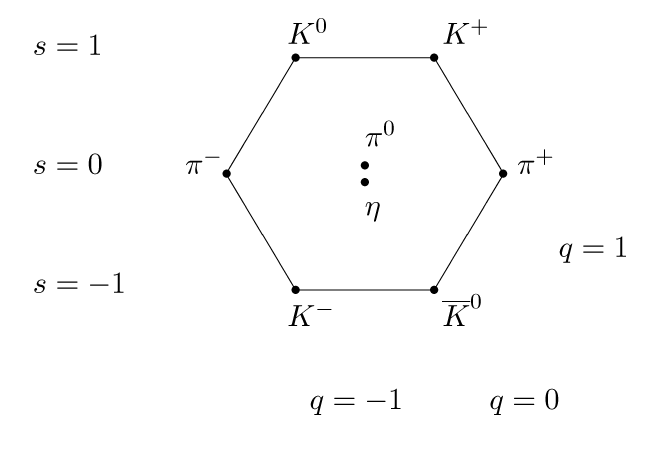
\includegraphics[scale=1]{Immagini/Meson_octet}
\caption{Gli otto mesoni dell'\emph{ottetto pseudoscalare}. Di ciascuno viene indicata la carica elettrica e la stranezza.}
\end{center}
\end{figure}

Nel seguito verrà trattato principalmente il comportamento dei kaoni neutri $K^0$ e $\bar{K}^0$, che presentano una serie di effetti quantomeccanici di notevole interesse.
Si tratta di particelle instabili, che condividono gli stessi canali di decadimento:
\begin{center}
\begin{tabular}{ll}
$K^0$ & $\rightarrow \pi^+ \pi^-$\\
 & $\rightarrow \pi^0 \pi^0$\\
 & $\rightarrow \pi^0 \pi^0 \pi^0$\\
 & $\rightarrow \pi^0 \pi^+ \pi^-$\\
 & $\rightarrow \pi^{\pm} \mu^{\mp} \nu_{\mu} (\bar{\nu_{\mu}})$\\
 & $\rightarrow \pi^{\pm} e^{\mp} \nu_{e} (\bar{\nu_{e}})$
\end{tabular}
\end{center}
\begin{center}
\begin{tabular}{ll}
$\bar{K^0}$ & $\rightarrow \pi^+ \pi^-$\\
 & $\rightarrow \pi^0 \pi^0$\\
 & $\rightarrow \pi^0 \pi^0 \pi^0$\\
 & $\rightarrow \pi^0 \pi^+ \pi^-$\\
 & $\rightarrow \pi^{\pm} \mu^{\mp} \nu_{\mu} (\bar{\nu_{\mu}})$\\
 & $\rightarrow \pi^{\pm} e^{\mp} \nu_{e} (\bar{\nu_{e}})$
\end{tabular}
\end{center}
Ciò, come verrà esposto nelle sezioni successive, è alla base del peculiare comportamento del sistema $K^0$ - $\bar{K}^0$. 

\section{Oscillazioni di stranezza}
\noindent
L'evoluzione temporale di un sistema di kaoni neutri presenta un effetto che non ha eguali in nessun altro tipo di sistema fisico (fatta eccezioni per i mesoni $D^0$, $B^0$ e 
$B_s$, che presentano notevoli analogie con i $K^0$): la trasformazione di una particella nella propria antiparticella.
Ciò è dovuto al fatto che $K^0$ e $\bar{K^0}$ non sono stati indipendenti ma possono oscillare l'uno nell'altro attraverso processi deboli virtuali intermedi del secondo ordine, ad esempio:
\begin{equation}
 K^0 \leftrightarrow \pi \pi \leftrightarrow \bar{K}^0
\end{equation}
Come risultato di questo accoppiamento, un fascio inizialmente puro di kaoni $K^0$ può essere osservato, ad un istante successivo, come miscela $K^0$ - $\bar{K}^0$.
Ne consegue che gli autostati di sapore $K^0$ e $\bar{K}^0$ non rappresentano la base più adatta per uno studio del sistema $K^0$ - $\bar{K}^0$ e, poiché ai tempi della scoperta
si credeva che ogni interazione dovesse conservare CP, venne naturale studiare tale sistema in funzione degli autostati di $\mathscr{C}\mathscr{P}$, $K_1$ e $K_2$:
\begin{equation}\label{K1}
|K_1\rangle=\frac{1}{\sqrt{2}} (|K^0\rangle + |\bar{K}^0\rangle)
\end{equation}
\begin{equation}\label{K2}
|K_2\rangle=\frac{1}{\sqrt{2}} (|K^0\rangle - |\bar{K}^0\rangle)
\end{equation}
Si verifica facilmente che:
\begin{equation}
 \mathscr{C}\mathscr{P}|K_1\rangle = |K_1\rangle
\end{equation}
\begin{equation}
\mathscr{C}\mathscr{P}|K_2\rangle = -|K_2\rangle 
\end{equation}
A questo punto, è necessario verificare il comportamento sotto $\mathscr{C}\mathscr{P}$ dei canali di decadimento, al fine di verificare quali di essi abbiano $CP = 1$
e quali $CP = -1$. Poiché, dal punto di vista sperimentale, lo studio dei decadimenti adronici è più agevole di quello relativo ai decadimenti semileptonici, ci si limiterà
a discutere i primi. Si considera dapprima il comportamento sotto $\mathscr{C}$ e $\mathscr{P}$ di un singolo pione. Valgono le seguenti relazioni:
\begin{equation}
 \mathscr{C}\psi(\pi^\pm) \rightarrow \psi(\pi^\mp)
\end{equation}
\begin{equation}
 \mathscr{C}\psi(\pi^0) \rightarrow \psi(\pi^0)
\end{equation}
\begin{equation}
 \mathscr{P}\psi(\pi) \rightarrow -\psi(\pi)
\end{equation}
dove, nell'ultima equazione, si è indicato con $\pi$ uno qualsiasi dei pioni $\pi^0$, $\pi^+$ o $\pi^-$, mentre il segno meno è dovuto al fatto che i pioni hanno parità 
intrinseca negativa. Dalle considerazioni appena fatte segue che, nel caso di sistema di due pioni si ha:
\begin {equation}
\mathscr{C}\mathscr{P}|\pi\pi\rangle = \mathscr{P}\mathscr{C}|\pi\pi\rangle = \mathscr{P}|\pi\pi\rangle = (-1)^2 (-1)^l |\pi\pi\rangle = |\pi\pi\rangle
\end{equation}
Nell'ultimo passaggio si è tenuto conto del fatto che i kaoni $K^0$ e $\bar{K}^0$ (quindi anche gli autostati di $\mathscr{C}\mathscr{P}$ $K_1$ e $K_2$) hanno spin 0 e quindi 
la conservazione del momento angolare impedisce ai prodotti di decadimento di avere momento angolare orbitale reciproco.
Quindi se ne conclude che:
\begin{equation}
 \mathscr{C}\mathscr{P}|\pi,\pi\rangle = |\pi,\pi\rangle
\end{equation}
Allo stesso modo, è possibile verificare che:
\begin{equation}
 \mathscr{C}\mathscr{P}|\pi,\pi,\pi\rangle = -|\pi,\pi,\pi\rangle
\end{equation}
In base al ragionamento fin qui fatto, i due autostati di $\mathscr{C}\mathscr{P}$ $K_1$ e $K_2$, devono decadere rispettivamente in due ed in tre pioni.
Quindi ci si attende che $K_2$ abbia una vita media sensibilmente più lunga del $K_1$, in quanto la maggior differenza di massa tra stati iniziali e stati 
finali favorisce il decadimento di quest'ultimo.

Le osservazioni sperimentali evidenziarono appunto, all'interno di un fascio di kaoni $K^0$ o $\bar{K}^0$, la presenza di due stati distinti, uno a vita media più breve,
per questo battezzato $K_S$ (\emph{K short}) ed uno a vita media più lunga, $K_L$ (\emph{K long}).
Le prime osservazioni sembrarono anche confermare il fatto che i decadimenti in due pioni erano caratteristici del $K_S$, mentre quelli in tre pioni del $K_L$, dando
un'importante conferma alla teoria del miscelamento dei kaoni $K^0$ e $\bar{K}^0$ negli autostati di CP chiamata anche, dai nomi dei due fisici che per primi la proposero,
\emph{teoria di Gell-Mann Pais}\cite{Kabir}. 

\section{Rigenerazione}
\noindent
Poiché le reazioni solitamente usate per la produzione di $K^0$:
\begin{equation}
 \pi^- + p \rightarrow \Lambda^0 + K^0
\end{equation}
\begin{equation}
 \pi^0 + n \rightarrow \Lambda^0 + K^0
\end{equation}
hanno una sezione d'urto significativa, si deduce, a causa del Teorema CPT, che i due processi:
\begin{equation}
\bar{K}^0 + p \rightarrow \Lambda^0 + \pi^+
\end{equation}
\begin{equation}
\bar{K}^0 + n \rightarrow \Lambda^0 + \pi^0
\end{equation}
debbano avere anch'essi una notevole sezione d'urto, così come le reazioni a queste simili nelle quali $\Lambda^0$ è sostituito da un iperione $\Sigma$. 
Ciò equivale a dire che i $\bar{K}^0$ reagiscono violentemente con la materia nucleare, dalla quale vengono assorbiti. 
Al contrario, i $K^0$ interagiscono molto più debolmente, spesso attraverso semplici urti elastici, risultando quasi completamente inerti.
Se si assume la validità della teoria di \emph{Gell-Mann Pais}, l'evoluzione di un sistema di kaoni neutri può essere descritta in termini dei due autostati di $\mathscr{CP}$, 
$K_S$ (il kaone neutro a vita breve) e $K_L$ (il kaone neutro a vita media lunga).

Si definiscono $\tau_S$ e $\tau_L$ le vite medie dei due stati, con $\tau_S << \tau_L$.
Un fascio di $K^0$ inizialmente puro, dopo un tempo $\tau$ tale per cui $\tau_S << \tau << \tau_L$, risulterà composto quasi esclusivamente da $K_L$:
\begin{equation}
 |K_L\rangle = \frac{1}{\sqrt{2}}\big(|K^0\rangle - |\bar{K}^0\rangle\big)
\end{equation}
mentre l'autostato $K_S$ potrà, sotto ogni aspetto pratico, essere considerato assente.
Ora si ponga sulla traiettoria del fascio un materiale di spessore tale che, nell'attraversamento di questo da parte dei $K_L$, si abbia una probabilità di interazione
da parte di un $\bar{K}^0$ prossima ad $1$. Questo materiale è, per i $\bar{K}^0$, qualcosa che approssima molto bene un assorbitore ideale, mentre i $K^0$ vengono trasmessi
senza attenuazioni. Il sistema, che era stato osservato come uno stato puro $K_L$ a monte dell'assorbitore, risulta quindi essere uno stato puro $K^0$ a valle di questo.
Ma questo ragionamento era iniziato appunto considerando un fascio puro di $K^0$, per cui si può iterare quanto detto finora e riesprimere questo come una sovrapposizione
$K_S$ e $K_L$. Il passaggio attraverso l'assorbitore ha quindi \emph{rigenerato} la componente $K_S$. 

Questo fenomeno, studiato e riprodotto sperimentalmente per la
prima volta da Pais e Piccioni, rappresenta una delle prime prove sperimentali della teoria del miscelamento tra gli autostati di sapore per opera dell'interazione debole \cite{Kabir}.

\section{Violazione di CP}
\begin{figure}
\begin{center}
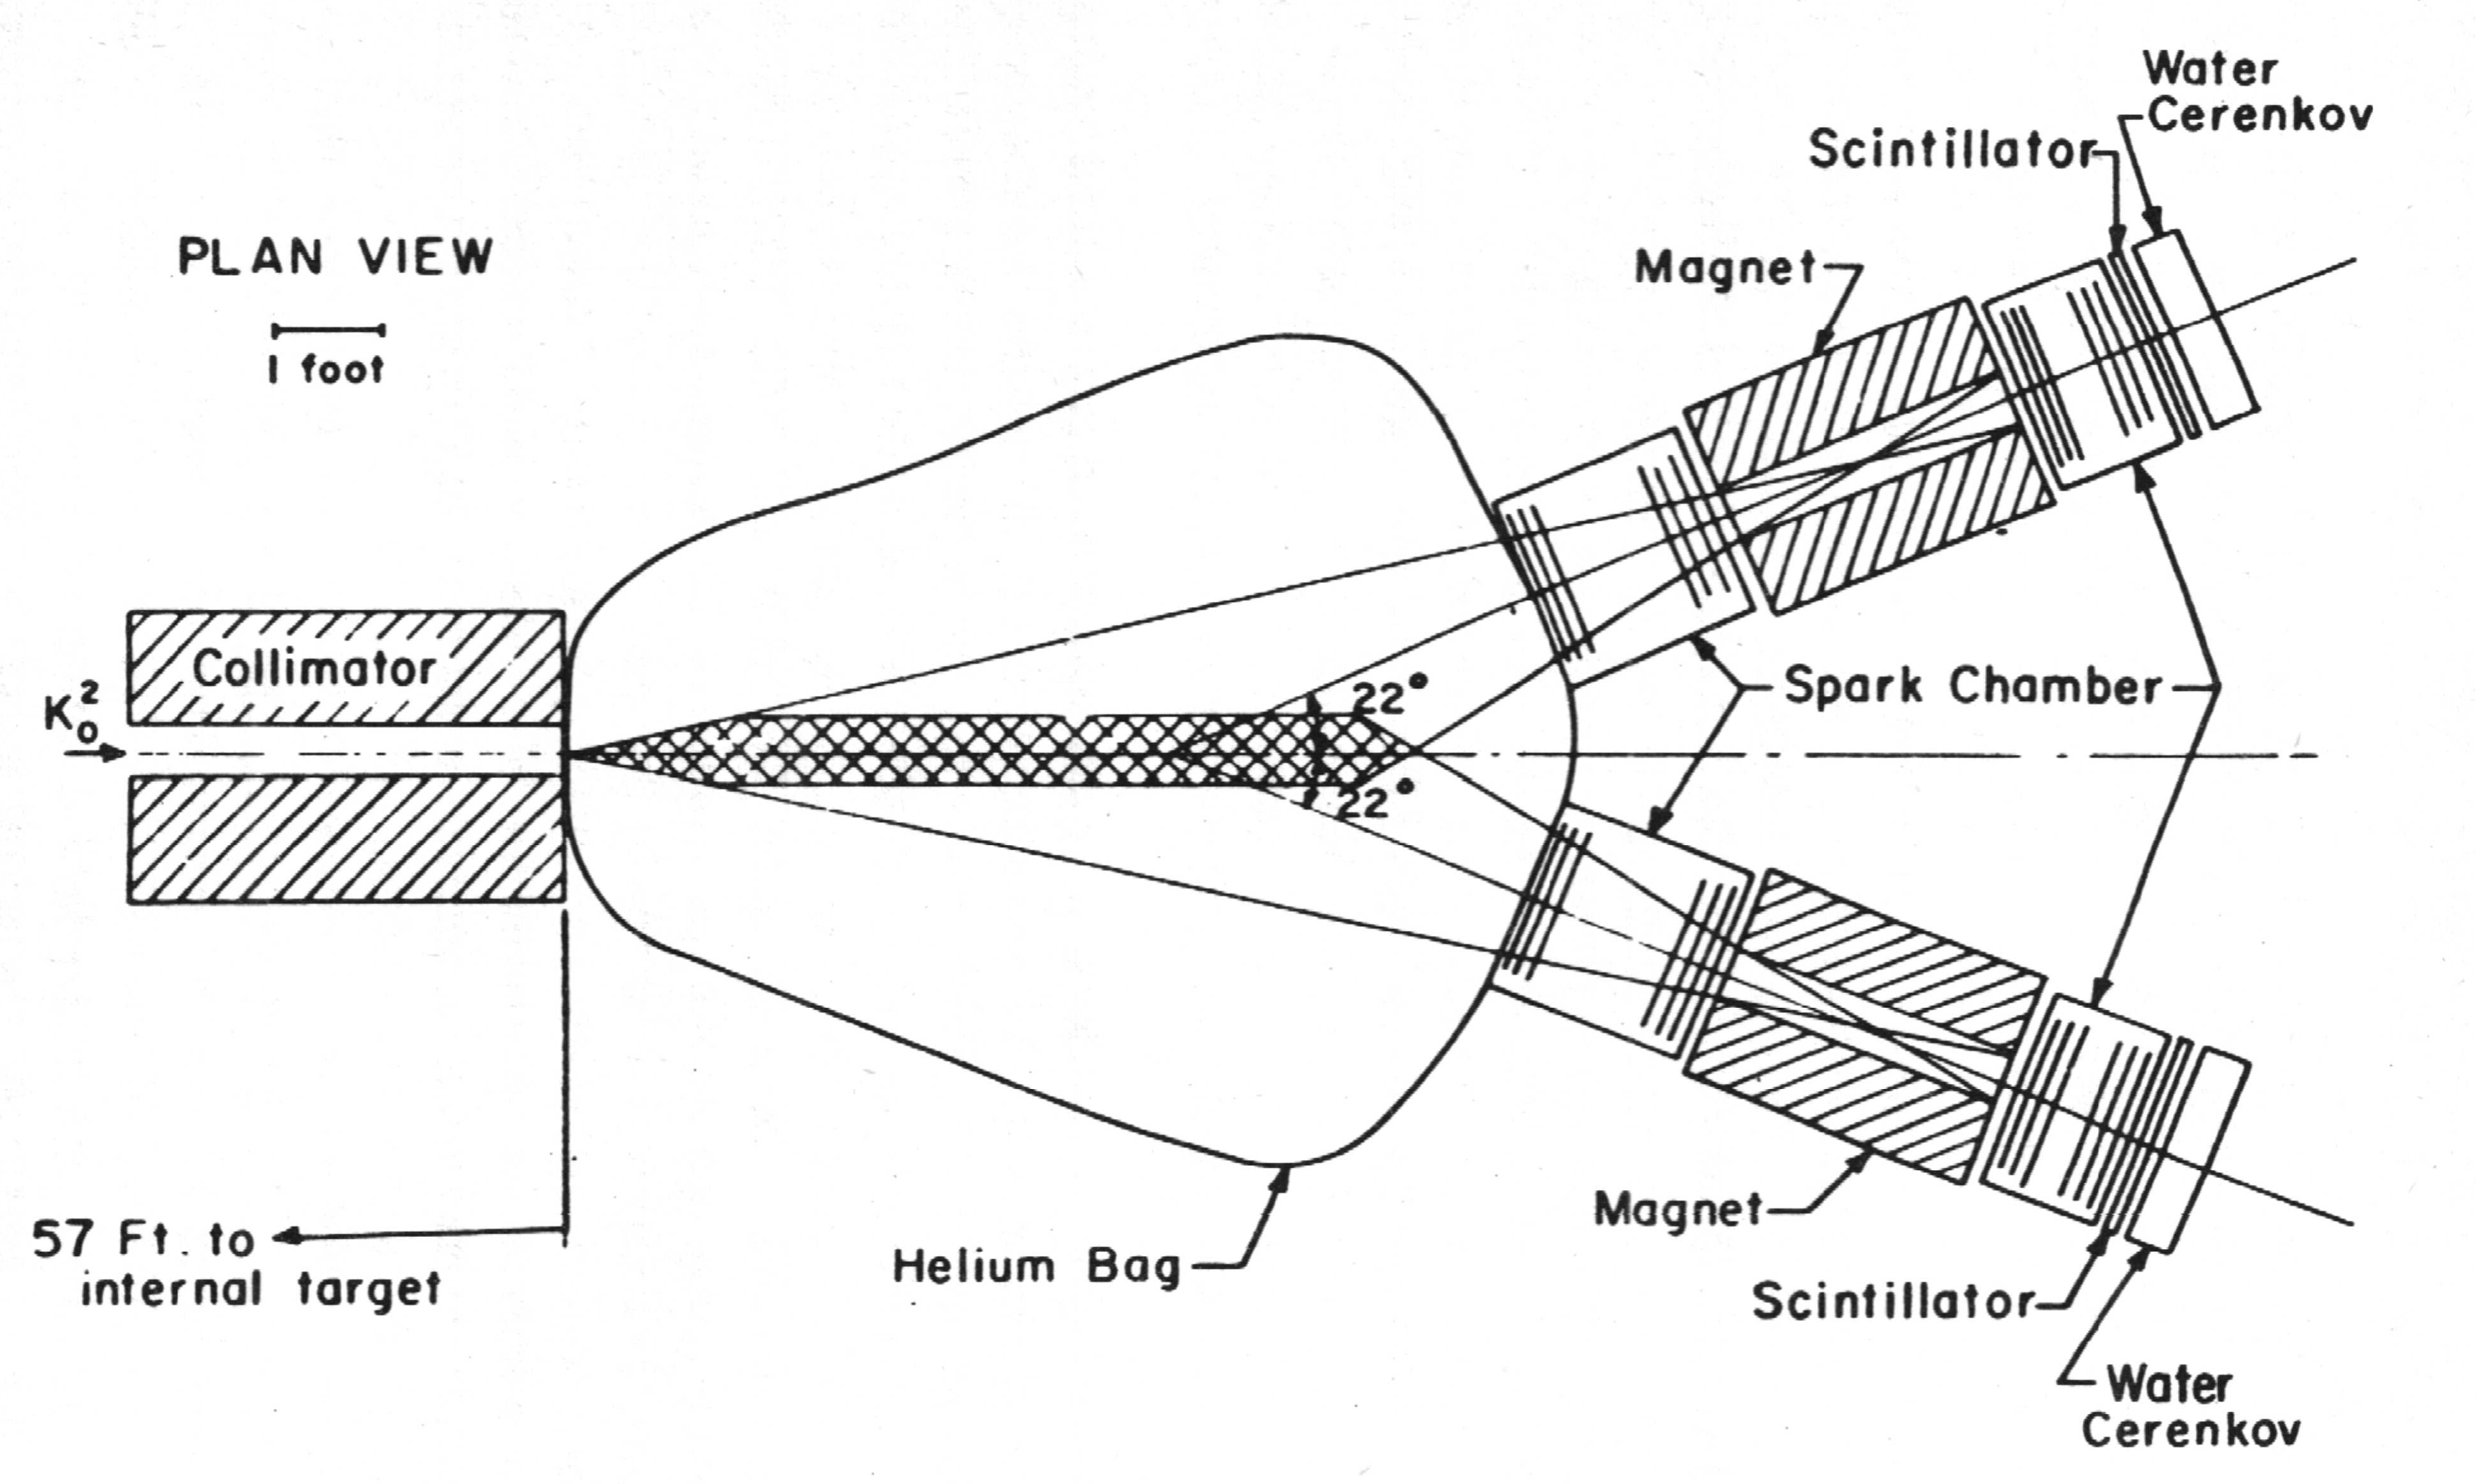
\includegraphics[scale=0.1]{Immagini/rilevatore}
\caption{Schema dell'apparato sperimentale impiegato da  Christenson, Cronin, Fitch e Turlay per l'osservazione del decadimento $K_L \longrightarrow \pi^+ \pi^-$}
\end{center}
\end{figure}
\noindent
Nel luglio del 1964 Christenson, Cronin, Fitch e Turlay annunciarono la sconcertante scoperta del decadimento:
\begin{equation}\label{CPviolation}
 K_L \longrightarrow \pi^+ \pi^-
\end{equation}
L'esperimento da loro allestito al Brookhaven National Laboratory, negli Stati Uniti, consisteva nel far percorrere ad un fascio di $K^0$ una distanza tale che la 
componente $K_S$ che raggiungeva il rilevatore fosse trascurabilmente piccola, quindi si studiavano i canali di decadimento del $K_L$.
Il canale \eqref{CPviolation} risultava avvenire con un \emph{branching ratio} pari a circa $0,3\%$, segno che nella dinamica del sistema $K^0$-$\bar{K}^0$
doveva esserci una violazione di CP a livello dello $0,3\%$ \cite{Krane}. 
Esattamente venne misurato il rapporto:
\begin{equation}
\frac{\Gamma (K_L\rightarrow \pi\pi)}{\Gamma (K_L\rightarrow all)} = (2,3 \pm 0,3) × 10^{−3}
 \end{equation}
In questo caso si parla di violazione di CP nel \emph{mixing}.
Un secondo metodo che venne proposto per testare la violazione di CP da parte del sistema dei kaoni neutri fu il confronto dei $rates$ di decadimenti
CP-coniugati, ad esempio:
\begin{equation}
 K_L \longrightarrow \pi^- \mu^+ \bar{\nu}_{\mu}
\end{equation}
\begin{equation}
 K_L \longrightarrow \pi^+ \mu^- \nu_{\mu}
\end{equation}
Se CP fosse una simmetria esatta i $rates$ dei due decadimenti dovrebbero essere identici, invece sperimentalmente questi risultarono differenti, 
ancora una volta di circa lo $0,3\%$, confermando il fatto che il sistema non fosse CP-invariante. In questo caso si parla di violazione di CP diretta \cite{Wong}.

A causa della violazione di CP, si dedusse anche che gli autostati di propagazione libera $K_L$ e $K_S$ non coincidono esattamente con gli autostati di CP $K_1$ e 
$K_2$ definiti dalle \eqref{K1} e \eqref{K2}, ma che fossero una sovrapposizione di entrambi:
\begin{equation}
    K_L = \frac{K_2 + \epsilon_1 K_1}{\sqrt{1+|\epsilon_1|^2}}  
\end{equation}
\begin{equation}
    K_S = \frac{K_1 + \epsilon_2 K_2}{\sqrt{1+|\epsilon_2|^2}}  
\end{equation}
dove $\epsilon_1$ ed $\epsilon_2$ sono due numeri complessi, che per il teorema CPT devono essere uguali ed il cui modulo è di ordine di grandezza pari all'entità di
violazione di CP ($\approx 10^{-3}$). \cite{Lee}

Per la scoperta della violazione di CP nel sistema $K^0$-$\bar{K}^0$, Cronin e Fitch ricevettero il Premio Nobel per la Fisica nel 1980.

     %%%%%%%%%%%%%%%%%%%%
     %                  %
     %  capitolo3.tex   %
     %                  %
     %%%%%%%%%%%%%%%%%%%%

\chapter{Evoluzione temporale di un sistema di mesoni neutri}
\noindent
In questo capitolo, dopo avere definito l'hamiltoniana efficace di un generico sistema di mesoni neutri ($K^0-\bar{K}^0$, $D^0-\bar{D}^0$, $B^0-\bar{B}^0$ o 
$B_s-\bar{B}_s$), 
si procederà alla soluzione del corrispondente problema agli autovalori.  Si studieranno le proprietà caratteristiche delle soluzioni ottenute, che descrivono i 
 fenomeni di oscillazione tra gli autostati di sapore ed il decadimento verso stati di particella non legati. Verrà definito infine il parametro, indicato 
con $\eta$, che misura l'entit\`a della violazione di $CP$, osservabile nell' evoluzione dello specifico sistema in esame.

Con i simboli $P^0$ e $\bar{P}^0$ si indicheranno nel seguito gli autostati di sapore corrispondenti alla generica coppia di mesoni $K^0-\bar{K}^0$, $D^0-\bar{D}^0$, $B^0-\bar{B}^0$ oppure $B_s-\bar{B}_s$.
%
%
\section{Approssimazione di Wigner-Weisskopf}
\noindent
Per descrivere l'evoluzione temporale di un sistema $P^0$-$\bar{P}^0$ si considera l'hamiltoniana totale:
\begin{equation}
 H = H_s + H_{em} + H_w
\end{equation}
dove con $H_s$ si è indicato il contributo dell'interazione forte, con $H_{em}$ quello dell'interazione elettromagnetica e con $H_w$ quello dell'interazione debole.
Considerate le proprietà di simmetria delle interazioni fondamentali valgono le seguenti regole di commutazione:
\begin{equation}
 [\mathscr{C}\mathscr{P},H_s] = [\mathscr{C}\mathscr{P},H_{em}] = 0
\end{equation}
in quanto CP è una simmetria esatta per le interazioni forti ed elettromagnetiche.

Da ciò segue che gli autostati di sapore $|P^0\rangle$ e $|\bar{P}^0\rangle$ sono anche autostati discreti di $H_s$ ed $H_{em}$. 
L'interazione debole $H_w$, che al contrario viola CP, è responsabile della transizione 
degli stati di \emph{flavour}: per decadimento, verso gli stati non legati $|k\rangle$, e per oscillazione 
$|P^0\rangle \leftrightarrow |\bar{P}^0\rangle$.
L'equazione di Schr{\"o}dinger associata al sistema è quindi:
\begin{equation}\label{schrod}
 i\frac{\partial}{\partial t}|\Psi(t)\rangle = (H_s + H_{em} + H_w)|\Psi(t)\rangle
\end{equation}
Per rimuovere la parte triviale della dipendenza temporale della funzione d'onda si introduce la funzione d'onda trasformata:
\begin{equation}\label{def}
 |\psi(t)\rangle = e^{it(H_s + H_{em})}|\Psi(t)\rangle
\end{equation}
In questo modo la \eqref{schrod} diventa:
\begin{equation}
 i\frac{\partial}{\partial t} |\psi(t)\rangle = e^{i(H_s + H_{em})t}H_w e^{-i(H_s + H_{em})t}|\psi(t)\rangle = H_w|\psi(t)\rangle
\end{equation}
Introduciamo ora le notazioni:
\begin{equation}
a(t) = \langle P^0|\psi(t)\rangle 
\end{equation}
\begin{equation}
 \bar{a}(t) = \langle \bar{P}^0|\psi(t)\rangle 
\end{equation}
\begin{equation}
c_k(t) = \langle k|\psi(t)\rangle
\end{equation}
L'evoluzione libera del sistema \`e definita dalle equazioni differenziali:
\begin{equation}\label{a}
 i\frac{d}{dt} a(t) = \langle P^0|H_w|P^0\rangle a(t) + \langle P^0|H_w|\bar{P}^0\rangle \bar{a}(t) + \sum_{k} \langle P^0|H_w|k\rangle c_k (t)
\end{equation}
\begin{equation}\label{b}
 i\frac{d}{dt} \bar{a}(t) = \langle \bar{P}^0|H_w|P^0\rangle a(t) + \langle \bar{P}^0|H_w|\bar{P}^0\rangle \bar{a}(t) + \sum_{k} \langle \bar{P}^0|H_w|k\rangle c_k (t)
\end{equation}
\begin{equation}\label{c}
 i\frac{d}{dt} c_k(t) = \langle k|H_w|P^0\rangle a(t) + \langle k|H_w|\bar{P}^0\rangle \bar{a}(t) + \sum_{k'} \langle k|H_w|k'\rangle c_{k'} (t)
\end{equation}
In questa forma le equazioni \eqref{a},\eqref{b},\eqref{c} descrivono l'evoluzione del sistema in maniera esatta.
Per ottenere una soluzione analitica si considera piccolo il contributo della serie che compare nella \eqref{c} rispetto ai due termini $\langle k|H_w|P^0\rangle a(t)$ e $\langle k|H_w|\bar{P}^0\rangle \bar{a}(t)$: 
ciò equivale a trascurare i contributi delle interazioni deboli tra i prodotti di decadimento (considerati dunque stabili). Questa approssimazione permette di riscrivere le equazioni nella forma seguente:
\begin{equation}\label{A8}
i\frac{d}{dt} \phi(t) = h_w \phi (t) + \sum_{k}{C_k}^* e^{-iw_kt} c_k (t)\\
\end{equation}
\begin{equation}\label{A9}
i\frac{d}{dt} c_k(t) = {C_k}^T \phi(t)e^{iw_kt}
\end{equation}
Dove si sono usate le notazioni:
\begin{equation}\label{1}
 \phi (t) = \binom{a(t)}{\bar{a}(t)}
\end{equation}
\begin{equation}\label{2}
 w_k = E_k - m_k
\end{equation}
\begin{equation}
 C_k = \binom{\langle k|H_w|P^0\rangle}{\langle k|H_w|\bar{P}^0\rangle}
\end{equation}
${C_k}^*$ e ${C_k}^T$ sono rispettivamente il vettore ottenuto eseguendo la complessa coniugazione degli elementi di $C_k$ ed il trasposto di 
$C_k$, mentre $h_w$ rappresenta la restrizione di $H_w$ al sottospazio generato da $P^0$ e $\bar{P}^0$.\\
Per la risoluzione delle equazioni \eqref{A8} e \eqref{A9} s'impongono le condizioni iniziali:
\begin{equation} \label{c1}
 \phi(0) = \phi_0
\end{equation}
\begin{equation}\label{c2}
 c_k(0) = 0
\end{equation}
dove la \eqref{c1} specifica la concentrazione iniziale di $P^0$ e $\bar{P}^0$, che in genere dipende dall'apparato sperimentale impiegato per la produzione del fascio. Con la \eqref{c2} si ipotizza che all'istante iniziale siano nulle le concentrazioni di tutti i possibili prodotti del decadimento.\\
La \eqref{A9} pu\`o essere risolta esplicitamente:
\begin{equation}
 c_k(t) = -i{C_k}^T\int_{0}^{t} \phi(0)e^{iw_k\tau}\, d\tau
\end{equation}
e quindi sostituita nella \eqref{A8}, in modo tale da eliminarne la dipendenza dai coefficienti $c_k(t)$:
\begin{equation}\label{kay}
 \frac{d}{dt} \phi(t) +ih_w\phi(t) = -\sum_{k}D_k\int_{0}^{t} \phi(\tau)e^{iw_k(t-\tau)} d\tau
\end{equation}
dove con $D_k$ si \`e indicata la matrice $2\times2$ definita dal prodotto tensoriale tra ${C_k}^*$ e ${C_k}^T$:
\begin{equation}\label{3}
 D_k = {C_k}^*\otimes{C_k}^T
\end{equation}
La \eqref{kay} pu\`o essere risolta utilizzando le trasformate di Laplace.\\
Si definisce la trasformata di $\phi$ come:
\begin{equation}
 \widetilde{\phi}(s) = \int_{0}^{\infty} \phi(t)e^{-ts} dt
\end{equation}
La trasformata del lato sinistro della \eqref{kay} \`e:
\begin{equation}
\int_{0}^{\infty} e^{-st}\frac{d}{dt}\phi(t) dt + ih_w\widetilde{\phi}(s) = \\
ih_w\widetilde{\phi}(s) + \phi(t)e^{-st}\Bigg|_{0}^{\infty} + s\int_{0}^{\infty} e^{-st}\phi(t)dt = \\
\end{equation}
\begin{equation}
= s\widetilde{\phi}(s) + ih\widetilde{\phi}(s) - \phi_0
\end{equation}
Mentre per il lato destro si ottiene:
\begin{equation}
 \int_{0}^{\infty} e^{-st}(\int_{0}^{t}\phi(\tau)e^{iw_k(t-\tau)} d\tau)dt = \int_{0}^{\infty}d\tau e^{iw_k\tau}\phi(\tau)\int_{\tau}^{\infty} e^{-(s+iw_k)t dt} =
\end{equation}
\begin{equation}
= \frac{\widetilde{\phi}(s)}{s + iw_k}
\end{equation}
Quindi si ottiene:
\begin{equation}
 s\widetilde{\phi}(s) + ih_w\widetilde{\phi}(s) - \phi_0 = - \sum_{k} D_k\frac{\widetilde{\phi}(s)}{s + iw_k}
\end{equation}
che ha per soluzione:
\begin{equation}\label{key}
 \widetilde{\phi}(s) = \frac{\phi_0}{s+iW(s)}
\end{equation}
dove si \`e definita la matrice $W(s)$ come:
\begin{equation}
 W(s) = h_w - \sum_{k} \frac{D_k}{w_k - is}
\end{equation}
Applicando la formula di inversione per le trasformate di Laplace a destra e a sinistra nella \eqref{key} si ottiene:
 \begin{equation}\label{inte}
 \phi(t) = \lim_{\epsilon\longrightarrow0}\frac{1}{2\pi i}\int_{-i\infty + \epsilon}^{i\infty + \epsilon} \frac{\phi_0e^{st}}{s+iW(s)}ds
 \end{equation}
Dove il termine $+\epsilon$ negli estremi sta ad indicare che il percorso di integrazione si trova immediatamente a destra dell'asse immaginario.
Si riesprime l'integrale \eqref{inte} in funzione di una nuova variabile reale $y$, definita attraverso la relazione $s = iy + \epsilon$:
\begin{equation}\label{int}
   \phi(t) = \lim_{\epsilon\longrightarrow0}\frac{1}{2\pi i}\int_{-\infty}^{\infty} \frac{\phi_0e^{i(y + \epsilon)t}}{iy + \epsilon+iW(iy + \epsilon)}dy
\end{equation}
Il maggior contributo all'integrale \eqref{int} si ha per $y\approx0$, cioè per valori piccoli dell'energia. 
Infatti, se si eccettua il contributo (costante) di $h$, $W$ è del secondo ordine in $H_w$ (essa dipende linearmente dalle 
matrici $D_k$ che, per come sono state definite, risultano del secondo ordine nelle $C_k$, a loro volta lineari in $H_w$).
Rappresenta dunque un'approssimazione ragionevole sostituire $W$ con il suo valore nell'origine:
\begin{equation}
 W\approx W_0 = W(0) = h - P(\sum_{k}\frac{D_k}{w_k}) - i\pi\sum_{k}\delta(w_k)D_k
\end{equation}
in cui si \`e utilizzata la \emph{formula di Sokhotski–Plemelj} (Appendice B).\\
In questo modo si ottiene una soluzione esplicita:
\begin{equation}
\phi = \frac{1}{2\pi i}\int_{-\infty}^{+\infty} \frac{\phi_0e^iyt}{y + W_0}dy = e^{-iW_0t} \phi_0
\end{equation}
che pu\`o essere espressa in forma differenziale nel modo seguente:
\begin{equation}
 i\frac{d}{dt}\phi = W_0\phi
\end{equation}
Ritornando alla funzione d'onda del sistema $P^0$-$\bar{P}^0$, tramite la relazione $\Phi = e^{-i(H_s + H_em)t}\phi$, si ottiene finalmente l'Hamiltoniana efficace del sistema, solitamente espressa nella forma seguente:
\begin{equation}
 i\frac{d}{dt}\Phi = \Bigg(M-\frac{i}{2}\Gamma\Bigg)\Phi 
\end{equation}
Dove si sono impiegate le notazioni:
\begin{equation}
M = m_k \mathbb{I} + h_w -P\sum_{k}\frac{D_k}{w_k}
\end{equation}
\begin{equation}
 \Gamma = 2\pi\sum_{k}D_k\delta(w_k)
\end{equation}
in cui con $\mathbb{I}$ si è indicata la matrice identità.

Si osserva che entrambe le matrici $M$ e $\Gamma$ sono Hermitiane, mentre $(M-\frac{i}{2}\Gamma)$ non lo è:
\begin{equation}
 \Bigg(M-\frac{i}{2}\Gamma\Bigg)^{\dag} = \Bigg(M +\frac{i}{2}\Gamma\Bigg) \neq \Bigg(M-\frac{i}{2}\Gamma\Bigg)
\end{equation}
Ricordando le sostituzioni \eqref{2}, \eqref{3} e la definizione di $h_w$ è possibile esplicitare gli elementi di $M$ e $\Gamma$:
\begin{equation}
M_{\mu\nu} = m_k\delta_{\mu\nu} + \langle \mu|H_w|\nu\rangle - P\sum_{k}\frac{\langle\mu|H_w|k\rangle\langle k|H_w|\nu\rangle}{E_k-m_k}
\end{equation}
\begin{equation}\label{gamma}
\Gamma_{\mu\nu} = 2\pi\sum_{k}\langle|\mu|H_w|k\rangle\langle k|H_w|\nu\rangle\delta(E_k-m_k) 
\end{equation}
in cui gli indici $\mu$ e $\nu$ indicano rispettivamente gli stati $P^0$ e $\bar{P}^0$.

Si ottiene dunque l'Hamiltoniana efficace:
\begin{equation}\label{Heff}
 H_{eff} = M -\frac{i}{2}\Gamma = \Big( \begin{matrix} M_{11} & M_{12} \\ M_{21} & M_{22} \end{matrix}\Big) - \frac{i}{2} \Big( \begin{matrix} \Gamma_{11} & \Gamma_{12} \\ \Gamma_{21} & \Gamma_{22} \end{matrix}\Big)
\end{equation}
dove $M$ \`e la \emph{matrice di massa}, i cui elementi diagonali $M_{11}$ e $M_{22}$ sono gli operatori di massa  dei due stati $P^0$ e $\bar{P}^0$, mentre gli elementi $M_{12}$ e $M_{21}$ regolano le oscillazioni tra gli stati. $\Gamma$ \`e la \emph{matrice di decadimento}, i cui termini diagonali $\Gamma_{11}$ e $\Gamma_{22}$ determinano le disintegrazioni dei due stati, mentre gli elementi $\Gamma_{12}$ e $\Gamma_{21}$ le loro oscillazioni.\\
%
% CPT
%
Come conseguenza diretta del Teorema CPT si ha $M_{11} = M_{22}$ e $\Gamma_{11} = \Gamma_{22}$.
Si verifica inoltre che $M_{12} = M_{21}^*$ e $\Gamma_{12} = \Gamma_{21}^*$.
%
Per riassumere, si è giunti a questi risultati in base ad alcune ipotesi che hanno permesso una notevole semplificazione del problema:
\begin{enumerate}
 \item All'istante iniziale il sistema \`e composto esclusivamente dai mesoni $P^0$ o $\bar{P}^0$ ($c_k(0) = 0$)
 \item Si trascurano gli effetti delle interazioni deboli tra i prodotti di decadimento dei mesoni neutri\\ 
 ($\sum_{k'} \langle k|H_w|k'\rangle c_{k'} (t) = 0$ nella \eqref{c})
 \item La dinamica temporale si riferisce solo all'evoluzione degli stati  ${P}^0$ e $\bar{P}^0$, definita dalle funzioni $a(t)$ e $\bar{a}(t)$.
 \item La scala dei tempi per la quale si osserva il sistema \`e grande rispetto ai tempi caratteristici delle interazioni forti ed elettromagnetiche ($y\approx0$ nell' integrale \eqref{int})
\end{enumerate}
Queste condizioni costituiscono quella che viene chiamata approssimazione di \emph{Wigner - Weisskopf} \cite{Kabir}.
%
% Autofunzioni e autovalori.
%
\section{Autofunzioni ed autovalori di $H_{eff}$}
\noindent
In questa sezione si risolverà il problema agli autovalori dell'Hamiltoniana efficace del sistema $P^0-\bar{P}^0$.
Si dimostrerà che l'evoluzione temporale del sistema consiste in una combinazione
di decadimento verso stati non legati e di oscillazioni tra gli autostati di \emph{flavour} definito  $|P^0\rangle$ e $|\bar{P^0}\rangle$.

Per semplicità di notazione si definiscono i parametri $\alpha$, $\beta_1$ e $\beta_2$ come:
\begin{equation}
\Big( \begin{matrix} M_{11}-\frac{i}{2}\Gamma_{11} & M_{12}-\frac{i}{2}\Gamma_{12} \\ M_{21}-\frac{i}{2}\Gamma_{21} & M_{22}-\frac{i}{2}\Gamma_{22} \end{matrix}\Big) = \Big( \begin{matrix} \alpha & \beta_1 \\ \beta_2 & \alpha  \end{matrix}\Big)
\end{equation}
Il problema agli autovalori per $H_{eff}$ ha come soluzione:
\begin{equation}
 |P_L\rangle = p|P^0\rangle + q|\bar{P}^0\rangle
\end{equation}
corrispondente all'autovalore $\mu_L = \alpha + \sqrt{\beta_1\beta_2}$, e
\begin{equation}
 |P_S\rangle = p|P^0\rangle - q|\bar{P}^0\rangle
\end{equation}
corrispondente all'autovalore $\mu_S = \alpha - \sqrt{\beta_1\beta_2}$.

Affinché gli autostati siano normalizzati, i coefficienti $p$ e $q$ devono soddisfare la relazione ${|p|}^2 +{|q|}^2 = 1$.
Si dimostra che essi valgono rispettivamente:
\begin{equation}
 p = \sqrt{\frac{\beta_1}{|\beta_1|+|\beta_2|}}
\end{equation}
\begin{equation}
 q = \sqrt{\frac{\beta_2}{|\beta_1|+|\beta_2|}}
\end{equation}
%
%
Contrariamente a quanto accade per gli stati $P^0$ e $\bar{P}^0$, che sono vincolati ad avere la stessa massa a causa del Teorema CPT, le masse degli autostati di 
propagazione libera $|P_L\rangle$ e $|P_S\rangle$ non hanno questa restrizione, infatti sperimentalmente risultano differenti.

A questo punto si cerca una forma diagonale per $H_{eff}$. 
\begin{equation}
V^{-1}H_{eff}V = \Big( \begin{matrix} \mu_L & 0 \\ 0 & \mu_S \end{matrix}\Big)
\end{equation}
La matrice diagonalizzante $V$ è definita da:
\begin{equation}
 V = \Big({|P_L\rangle}^T , {|P_S\rangle}^T\Big) = \Big( 
\begin{matrix} p & p \\ q & -q \end{matrix} \Big) = \frac{1}{\sqrt{|\beta_1|+|\beta_2|}}\Big( 
\begin{matrix} \sqrt{\beta_1} & \sqrt{\beta_1} \\ \sqrt{\beta_2} & -\sqrt{\beta_2} \end{matrix}\Big)
\end{equation}
Si osserva che, a causa della non hermitianità di $H_{eff}$, $V$ non è una matrice unitaria. 
Per la stessa ragione, gli autovalori $\mu_L$ e $\mu_S$ non saranno reali, ma risulteranno entrambi complessi.

Ricordando l'equazione di Schr\"{o}dinger associata al sistema:
\begin{equation}
i\frac{d}{dt} \binom{a(t)}{\bar{a}(t)} = H_{eff} \binom{a(t)}{\bar{a}(t)}
\end{equation}
si ottiene:
\begin{equation*}
 i\frac{d}{dt} \binom{a(t)}{\bar{a}(t)} = V[V^{-1}H_{eff}V]V^{-1} \binom{a(t)}{\bar{a}(t)}
\end{equation*}
\begin{equation}
 i\frac{d}{dt} \Big[V^{-1}\binom{a(t)}{\bar{a}(t)}\Big] = [V^{-1}H_{eff}V] \Big[V^{-1}\binom{a(t)}{\bar{a}(t)}\Big]
\end{equation}
(nell'ultimo passaggio si è sfruttata l'indipendenza dal tempo della matrice diagonalizzante per poterla portare sotto l'operazione di derivata)

Definendo ora il vettore trasformato:
\begin{equation}
 \binom{l(t)}{s(t)} = V^{-1}\binom{a(t)}{\bar{a}(t)} 
\end{equation}
si ottiene la forma diagonale dell'equazione di Schr\"{o}dinger per il sistema dei mesoni neutri:
\begin{equation}
 i\frac{d}{dt}\binom{l(t)}{s(t)} = \Big( \begin{matrix} \mu_L & 0 \\ 0 & \mu_S \end{matrix}\Big) \binom{l(t)}{s(t)}
\end{equation}
Quest'equazione ammette la soluzione esplicita:
\begin{equation}\label{soluzione}
 \binom{l(t)}{s(t)} = \binom{l(0)e^{-i\mu_Lt}}{s(0)e^{-i\mu_St}}
\end{equation}
La soluzione nella base iniziale è data dalla trasformazione inversa della \eqref{soluzione}:
\begin{equation}
  \binom{a(t)}{\bar{a}(t)} = V\binom{l(t)}{s(t)} = \frac{1}{\sqrt{|\beta_1|+|\beta_2|}} \binom{\sqrt{\beta_1}[l(0)e^{-i\mu_Lt} + s(0)e^{-i\mu_St}]}{\sqrt{\beta_2}[l(0)e^{-i\mu_Lt} + s(0)e^{-i\mu_St}]}
\end{equation}
Finalmente è possibile scrivere la funzione d'onda del sistema:
\begin{equation}
 |\psi(t)\rangle = \sqrt{\frac{\beta_1}{|\beta_1|+|\beta_2|}} \Big[l(0)e^{-i\mu_Lt}+s(0)e^{-i\mu_St}\Big]|P^0\rangle + \sqrt{\frac{\beta_2}{|\beta_1|+|\beta_2|}}\Big[l(0)e^{-i\mu_Lt}-s(0)e^{-i\mu_St}\Big]|\bar{P}^0\rangle
\end{equation}

Il problema pi\`u interessante dal punto di vista sperimentale consiste nello studio dell'evoluzione temporale di un fascio di mesoni inizialmente puro, che all'istante $t = 0$ sia composto cio\`e esclusivamente da $P^0$ o da $\bar{P}^0$. \\
Si ricordano le definizioni degli autovalori dell'Hamiltoniana efficace:
\begin{equation}
\mu_L =  \alpha + \sqrt{\beta_1\beta_2} = (M_{11} - \frac{i}{2} \Gamma_{11}) + \sqrt{(M_{12} - \frac{i}{2} \Gamma_{12})(M_{21} - \frac{i}{2} \Gamma_{21})}
\end{equation}
\begin{equation}
\mu_S =  \alpha - \sqrt{\beta_1\beta_2} = (M_{11} - \frac{i}{2} \Gamma_{11}) - \sqrt{(M_{12} - \frac{i}{2} \Gamma_{12})(M_{21} - \frac{i}{2} \Gamma_{21})}
\end{equation}
Si definiscono a partire da questi le masse efficaci $m_L$ ed $m_S$ e le ampiezze di decadimento efficaci $\Gamma_L$ e $\Gamma_S$:
\begin{equation}
m_L = \Re\{\mu_L\} \ \ \ \ \ \ \ \ \ \ \ \ \ \ \gamma_L = -\frac{1}{2}\Im\{\mu_L\} 
\end{equation}
\begin{equation}
m_S = \Re\{\mu_S\} \ \ \ \ \ \ \ \ \ \ \ \ \ \ \gamma_S = -\frac{1}{2}\Im\{\mu_S\} 
\end{equation}
L'evoluzione temporale dei due sistemi diventa:
\begin{equation}
 |P^0\rangle = f_+(t) |P^0\rangle + \frac{q}{p}f_-(t) |\bar{P}^0\rangle 
\end{equation}
\begin{equation}
 |\bar{P}^0\rangle = \frac{p}{q}f_+(t) |P^0\rangle + f_-(t) |\bar{P}^0\rangle 
\end{equation}
dove si sono usate le notazioni compatte:
\begin{equation}
 f_+(t) = \frac{1}{2} \Big[e^{-im_Lt}e^{-\frac{\gamma_L}{2}t} + e^{-im_St}e^{-\frac{\Gamma_S}{2}t}\Big]
\end{equation}
\begin{equation}
 f_-(t) = \frac{1}{2} \Big[e^{-im_Lt}e^{-\frac{\gamma_L}{2}t} - e^{-im_St}e^{-\frac{\Gamma_S}{2}t}\Big]
\end{equation}
Appare evidente ciò che accade a un sistema puro, preparato con soli $|P^0\rangle$ oppure $\bar{|P^0}\rangle$ all'istante $t = 0$ : per effetto dei processi deboli 
del secondo ordine si verificano le oscillazioni , in maniera tale che ad un istante $t>0$ nel fascio sono presenti entrambi gli autostati di \emph{flavour}. 
A queste oscillazioni si sovrappone il decadimento esponenziale dei due mesoni \cite{Lee}.
\begin{figure}
\begin{center}
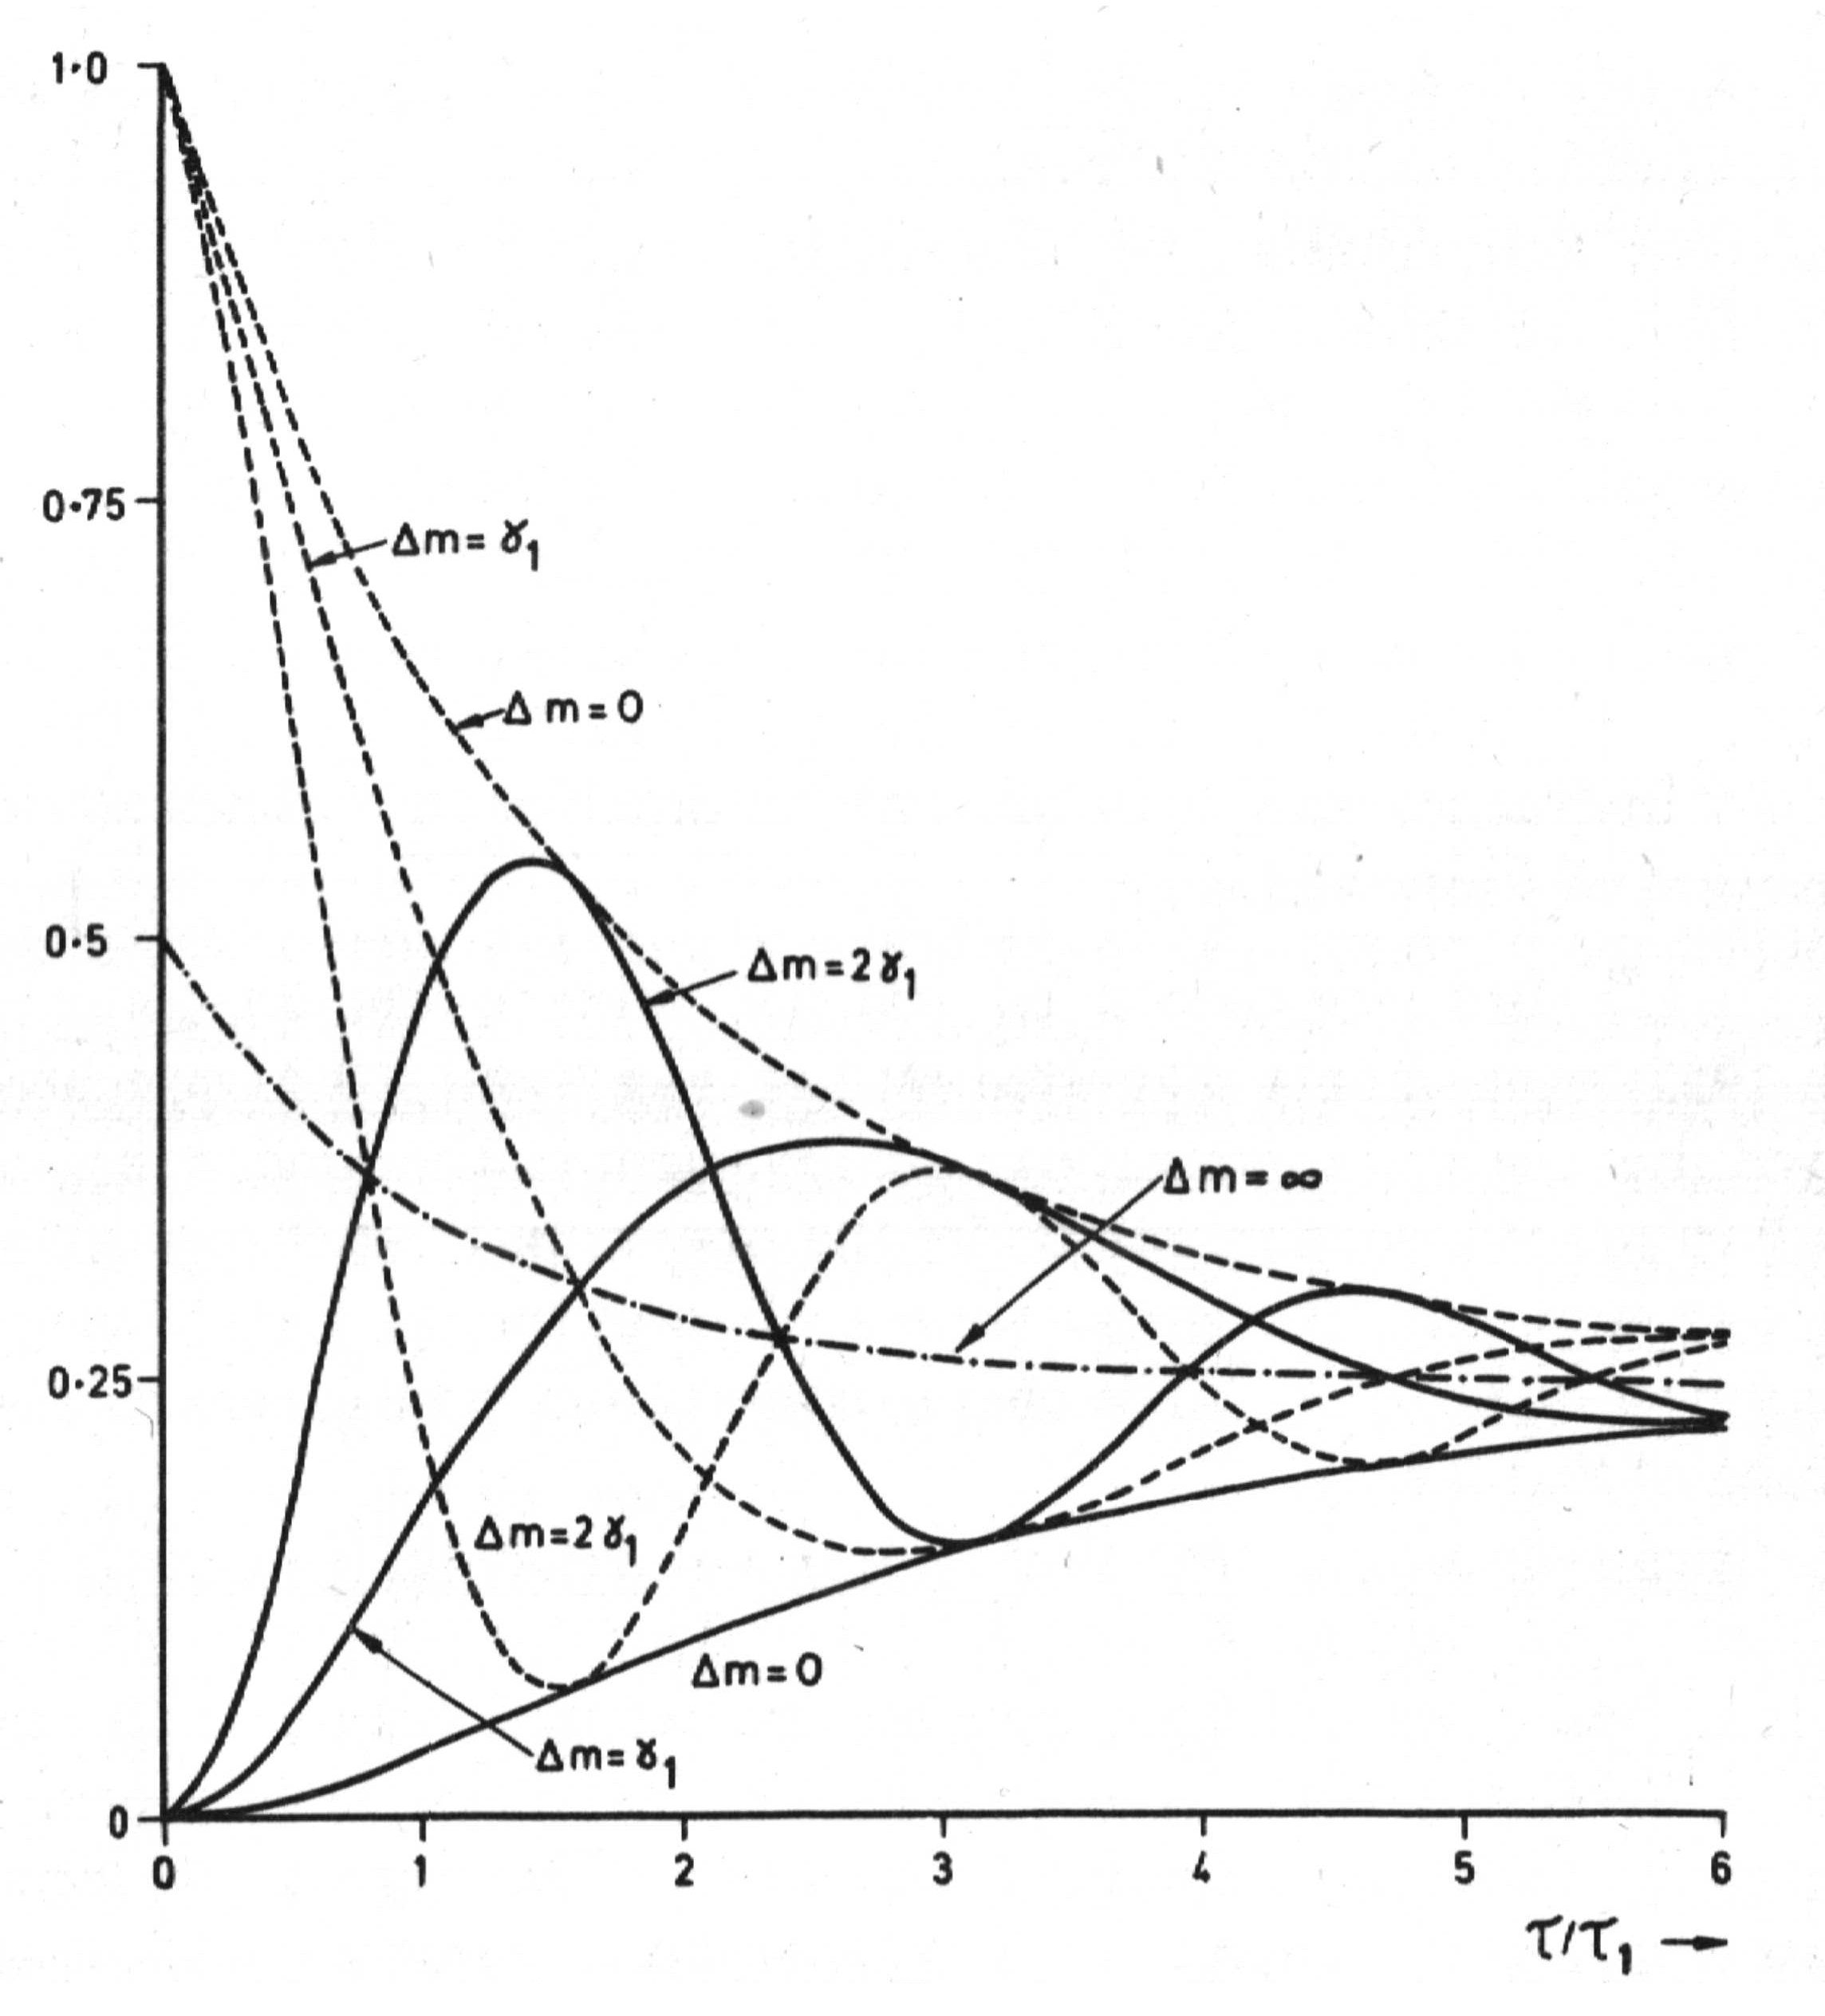
\includegraphics[scale=0.09]{Immagini/oscillazioni}
\caption{Probabilità di trovare un $P^0$ o un $\bar{P}^0$ in un fascio inizalmente costituito dal solo $P^0$ in funzione del tempo, per vari valori di $\Delta m$, la differenza
di massa tra i due autostati di propagazione $P_L$ e $P_S$ \cite{Kabir}.}
\end{center}
\end{figure}

\section{Violazione di CP}
\noindent
In questo paragrafo si studierà la violazione di CP del sistema dei mesoni neutri. Si premette la dimostrazione di due risultati
che saranno fondamentali per la discussione successiva.
\begin{teorema}
 Se il sistema dei mesoni neutri è invariante per CPT allora, indipendentemente dall'invarianza per T, valgono le relazioni:
\begin{equation}\label{teo1a}
 |P_S\rangle = \binom{1+\epsilon}{1-\epsilon} \frac{1}{\sqrt{2(1+{|\epsilon|}^2)}}
\end{equation}
\begin{equation}\label{teo1b}
 |P_L\rangle = \binom{1+\epsilon}{\epsilon-1} \frac{1}{\sqrt{2(1+{|\epsilon|}^2)}}
\end{equation}
dove $\epsilon \in \mathbb{C}$.
\end{teorema}
\begin{proof}
Consideriamo la matrice $H_{eff}$ \eqref{Heff}. Essendo questa una matrice $2 \times 2$ ad elementi complessi, è sempre possibile esprimerla come:
\begin{equation} \label{unimport}
 H_{eff} = D\mathbb{I} + \sum_{i=1}^{3}E_i\sigma_i
\end{equation}
dove $D, E_i \in \mathbb{C}$ sono costanti, mentre le $\sigma_i$ sono le matrici di Pauli \eqref{sigma1}, \eqref{sigma2}, \eqref{sigma3}.
Come è stato già evidenziato, a causa del Teorema CPT gli elementi sulla diagonale principale dell'Hamiltoniana efficace sono tra loro uguali.
Questo porta necessariamente a $E_3 = 0$.
Posto $E_1 = E \cos (\alpha)$ e $E_2 = E\sin(\alpha)$, con $E \in \mathbb{C}$ e $\alpha \in [0,2\pi]$, l'equazione \eqref{unimport} diventa:
\begin{equation}
 H_{eff} = D\mathbb{I} + E \Bigg(\begin{matrix} 0 & e^{-i\alpha} \\ e^{i\alpha} & 0 \end{matrix}\Bigg)
\end{equation}
Si verifica che gli autovettori sono:
\begin{equation}\label{eti}
 \binom{1}{e^{i\alpha}}\ \ \ \ \ \ \ \ \ \ \ \ \ \ \ \binom{1}{-e^{i\alpha}}
\end{equation}
Introducendo la notazione:
\begin{equation}
 e^{i\alpha} = \frac{1 - \epsilon}{1+\epsilon}
\end{equation}
gli autovettori \eqref{eti} diventano:
\begin{equation}
 \binom{1+\epsilon}{1-\epsilon}\ \ \ \ \ \ \ \ \ \ \ \ \ \ \ \binom{1+\epsilon}{\epsilon-1}
\end{equation}
che, divisi per gli opportuni coefficienti di normalizzazione, coincidono con le espressioni \eqref{teo1a} e \eqref{teo1b}.
\end{proof}
%
%
\begin{teorema}
 Se il sistema dei mesoni neutri è invariante per T allora, indipendentemente dall'invarianza per CPT, valgono le relazioni:
\begin{equation}
 |P_S\rangle = \binom{1+\delta}{1-\delta} \frac{1}{\sqrt{2(1+{|\delta|}^2}}
\end{equation}
\begin{equation}
 |P_L\rangle = \binom{1-\delta}{-(1+\delta)} \frac{1}{\sqrt{2(1+{|\delta|}^2}}
\end{equation}
dove $\delta\in \mathbb{C}$.
\end{teorema}
%
\begin{proof}
Per ipotesi la dinamica del sistema è invertibile rispetto all'inversione temporale. Ciò equivale a chiedere:
\begin{equation}
 \langle P_L|M-\frac{i}{2}\Gamma|P_S\rangle = \langle P_S|\mathscr{T}^{-1}(M-\frac{i}{2}\Gamma)\mathscr{T}|P_L\rangle = \langle P_S|M-\frac{i}{2}\Gamma|P_L\rangle
\end{equation}
Ricordando che $|P_L\rangle$ e $|P_S\rangle$ sono autostati dell'Hamiltoniana efficace di autovalori $\mu_L$ e $\mu_S$ si ottiene:
\begin{equation}
 \mu_S \langle P_L|P_S\rangle = \mu_L \langle P_S|P_L\rangle
\end{equation}
Poiché si è dimostrato che $\mu_L \neq \mu_S$, mentre $\langle P_L|P_S\rangle = \langle P_S|P_L\rangle$ si ottiene:
\begin{equation}
 \langle P_L|P_S\rangle = 0
\end{equation}
Due vettori complessi mutualmente ortogonali possono essere parametrizzati nel modo seguente:
\begin{equation}\label{q}
 |P_S\rangle \varpropto \binom{1 + \delta}{1 - \delta}
\end{equation}
\begin{equation}\label{w}
 |P_L\rangle \varpropto \binom{1 - \delta}{-(1 + \delta)}
\end{equation}
con $\delta \in \mathbb{C}$. Le relazioni \eqref{q} e \eqref{w}, divise per gli opportuni fattori di normalizzazione, forniscono la prova dell'asserto. 
\end{proof}
%
% eta
%
A questo punto si definisce il parametro $\eta$ nel modo seguente:
\begin{equation}
 \eta = \langle P_S|P_L\rangle
\end{equation}
in base ai risultati dei due teoremi appena dimostrati si deduce che 
\begin{displaymath}
\left\{
\begin{array}{l}
CPT \Longrightarrow \eta  \ reale\\
T \Longrightarrow \eta \    immaginario
\end{array}
\right.
\end{displaymath}
Infatti se il sistema \`e invariante per CPT dal Teorema 2.1si ha:
\begin{equation} 
\langle P_S|P_L\rangle = \frac{\epsilon + \epsilon^*}{1 + (|\epsilon|)^2}
\end{equation}
mentre se \`e invariante dal Teorema 2.2 per T:
\begin{equation}
 \langle P_S|P_L\rangle = \frac{\delta^* - \delta}{1 + (|\delta|)^2}
\end{equation}
Per cui $\eta$ si rivela un ottimo parametro per valutare la violazione di CP (che, per il teorema CPT, avviene se viene violata T).
Se entrambe le simmetrie CPT e CP fossero esatte, allora si dovrebbe avere $\eta = 0$ e i due autostati $|P_S\rangle$ e $|P_L\rangle$
si ridurrebbero agli autostati dell'operatore $\mathscr{C}\mathscr{P}\ |P_1\rangle$ e $|P_2\rangle$ definiti, nel caso dei kaoni, dalle espressioni \eqref{K1} e \eqref{K2}.
Il parametro $\eta$ può essere calcolato a partire dagli elementi delle matrici di massa e di decadimento. Dato il problema agli autovalori per l'hamiltoniana efficace:
\begin{equation}
(M - i \frac{\Gamma}{2})|P_j\rangle = (m_j - \frac{i}{2} \gamma_j) |P_j\rangle
\end{equation}
Dove $j$ è un indice che può significare $L$ o $S$.
Moltiplicando per l'unità immaginaria i due lati di questa espressione ed eseguendo il prodotto scalare per il bra $\langle P_k|$ (con $k = L, S$) si ottengono le relazioni:
\begin{equation}
 \langle P_S | \frac{\Gamma}{2} + iM | P_L \rangle = (\frac{1}{2} \gamma_L + i m_L) \langle P_S |P_L\rangle 
\end{equation}
\begin{equation} \label{questa}
 \langle P_L | \frac{\Gamma}{2} + iM | P_S \rangle = (\frac{1}{2} \gamma_S + i m_S) \langle P_L |P_S\rangle 
\end{equation}
L'espressione hermitiana coniugata dell'equazione precedente è:
\begin{equation}
 \langle P_L | \frac{\Gamma}{2} - iM | P_S \rangle = (\frac{1}{2} \gamma_S - i m_S) \langle P_L |P_S\rangle 
\end{equation}
che, sommata alla \eqref{questa}, diventa:
\begin{equation}
 2\langle P_S |\Gamma | P_L \rangle = [\frac{1}{2} (\gamma_L + \gamma_S) + i(m_L - m_s)] \eta
\end{equation}
 dove si è usata la definizione $\eta = \langle P_S|P_L \rangle$.
È possibile dimostrare \cite{Lee} la seguente identità:
\begin{equation}
 \langle P_S |\Gamma |P_L \rangle = \frac{1}{2} \sum_c \sqrt{\gamma_S(c)\gamma_L(c)} e^{i\theta_c}
\end{equation}
dove $c$ è un indice che identifica gli stati di decadimento finali, mentre $\phi$ è una generica fase.
Quindi si ottiene la seguente espressione di $\eta$:
\begin{equation}
 \eta = \frac{\sum_c \sqrt{\gamma_S(c)\gamma_L(c)} e^{i\theta_c}}{\frac{1}{2} (\gamma_L + \gamma_S) + i (m_L - m_S)}
\end{equation}
attraverso la quale è possibile quantificare l'entità della violazione di CP in ciascuno dei sistemi $P^0$ - $\bar{P}^0$.
     %%%%%%%%%%%%%%%%%%%%
     %                  %
     %  capitolo4.tex   %
     %                  %
     %%%%%%%%%%%%%%%%%%%%

\chapter{Violazione di CP nel Modello Standard}
\section{Teoria del $quark$ $mixing$ e matrice CKM}
\noindent
All'inizio degli anni sessanta Gell-Mann introdusse per la prima volta l'ipotesi dell'esistenza dei quark. La teoria originale prevedeva 
tre sapori: $up$, $down$ e $strange$. I campi \emph{left-handed} dei quark $up$ e $down$ vennero associati ad un doppietto elettrodebole, gli altri
a dei singoletti:
\begin{equation}
 \binom{u}{d}_L;\;u_R;\;d_R;\;s_L;\;s_R
\end{equation}
\begin{figure}
\begin{center}
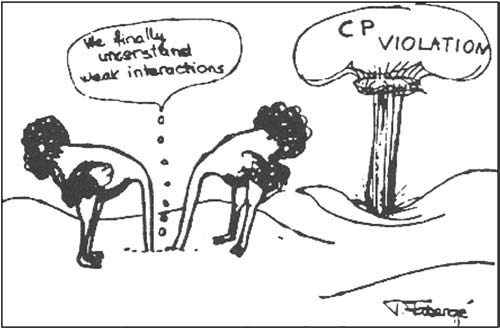
\includegraphics[scale=0.7]{Immagini/vignetta}
\caption{Vignetta presentata da Nicola Cabibbo nel 1966. La violazione di CP, non prevista dai modelli di \emph{quark mixing} teorizzati fino ad allora, viene rappresentata come una potente esplosione, in grado di scuotere le fondamenta della fisica teorica dell'epoca.}
\end{center}
\end{figure}

\subsection{Teoria di Cabibbo}
\noindent
Nel 1963, N. Cabibbo ipotizzò che una rottura spontanea della simmetria portasse ad un $mixing$ dei campi $d_L$ ed $s_L$, portando ad una
espressione della corrente carica della forma:
\begin{equation}\label{Cab}
 J^1_{\mu} + iJ^2_{\mu} = \bar{u}_L\gamma_\mu (\cos(\theta)d_L + \sin(\theta)s_L)
\end{equation}
dove $\theta$ viene detto angolo di Cabibbo. Questa ipotesi, unita ad alcune considerazioni derivanti dalla teoria delle interazioni forti, 
permise di ottenere un ottimo accordo con i dati sperimentali riguardanti le disintegrazioni $\beta$ di adroni con e senza stranezza.
Tuttavia questa teoria permette l'esistenza di correnti deboli neutre con cambiamento di sapore (cioè di stranezza, in questo semplice schema
a tre quark), il che è in contrasto con i dati sperimentali \cite{Maiani}. Infatti la \eqref{Cab} può essere riscritta nel modo seguente:
\begin{equation}
  J^1_{\mu} + iJ^2_{\mu} = \bar{q}_L C \gamma_\mu q_L = \bar{q}_L \Bigg(\begin{matrix} 0 & \cos(\theta) & \sin(\theta) \\ 0 & 0 & 0 \\ 0 & 0 & 0 \end{matrix}\Bigg) \gamma_\mu q_L
\end{equation}
È possibile dimostrare che la corrente elettrodebole neutra coinvolge il commutatore $[C, C^{\dag}]$. Se questo risulta essere non diagonale, 
sono possibili correnti deboli con cambiamento di sapore. Nel caso sopra esposto si ha:
\begin{equation}
 [C, C^{\dag}] = \Bigg(\begin{matrix} 1 & 0 & 0 \\ 0 & -\cos^2(\theta) & -sin(\theta)\cos(\theta) \\ 0 & -\sin(\theta)\cos(\theta) & -\sin^2(\theta) \end{matrix}\Bigg)
\end{equation}

\subsection{Teoria di Glashow, Iliopoulos e Maiani}
\noindent
La difficoltà insita nella teoria di Cabibbo venne superata nel 1970 con l'ipotesi dell'esistenza di un quarto quark, oggi chiamato $charm$,
avente le stesse proprietà elettrodeboli del quark $up$.
In questo modo, i campi \emph{left-handed} dei quark $up$ e $down$ continuano a formare un doppietto elettrodebole, un secondo doppietto è formato
dai campi \emph{left-handed} dei quark $charm$ e $strange$, mentre gli altri campi rappresentano singoletti elettrodeboli:
\begin{equation}
 \binom{u}{d}_L;\;\binom{c_L}{s_L}_L;\;u_R;\;d_R;\;c_R;\;s_R
\end{equation}
Ora $C$ è una matrice $4×4$ e la corrente debole carica prende la forma:
\begin{equation}
 J^1_{\mu} + iJ^2_{\mu} = \bar{q}_L \Bigg(\begin{matrix} 0 & U_{GIM} \\ 0 & 0 \end{matrix}\Bigg)
\end{equation}
dove si è indicata con $U_{GIM}$ la matrice:
\begin{equation}
U_{GIM} = \Bigg(\begin{matrix} \cos(\theta) & \sin(\theta) \\ -\sin(\theta) & \cos(\theta) \end{matrix}\Bigg)
\end{equation}
A causa dell'unitarietà di $U_{GIM}$, il commutatore $[C. C^{\dag}]$ è completamente diagonale:
\begin{equation}
 [C. C^{\dag}] = \Bigg(\begin{matrix} U_{GIM}U_{GIM}^\dag & 0 \\ 0 & -U_{GIM}^\dag U_{GIM} \end{matrix}\Bigg) = \Bigg(\begin{matrix} 1 & 0 \\ 0 & -1 \end{matrix}\Bigg)
\end{equation}
quindi, in accordo con i dati sperimentali, non sono consentite correnti elettrodeboli neutre con cambiamento di sapore \cite{Maiani}.

\subsection{Teoria di Kobayashi-Maskawa}
\noindent
Nel 1973 la validità del meccanismo di Glashow, Iliopoulos e Maiani e la conseguente esistenza del quark $charm$ erano ampiamente accettate dai fisici
teorici. Tuttavia la violazione di CP, osservata per la prima volta nel decadimento dei kaoni neutri nel 1964 e che da allora
era stata ampiamente studiata, non era prevista da tale meccanismo.
Il modo più naturale per avere una violazione di CP è quello di avere una fase complessa all'interno della matrice di \emph{mixing}\cite{Kobayashi}.
Tuttavia è immediato verificare che una eventuale fase complessa presente nella matrice $U_{GIM}$ può sempre essere eliminata sfruttando 
l'arbitrarietà nella fase del campo associato a ciascun quark.
Kobayashi e Maskawa calcolarono la dimensione minima che una matrice di \emph{mixing} doveva possedere affinché risultasse impossibile eliminare
tutte le fasi.
\begin{teorema}
Una matrice di \emph{mixing} $V$ di dimensione $N$ contiene $\frac{1}{2}(N-1)(N-2)$ fasi irriducibili.
\end{teorema}
\begin{proof}
 Una generica matrice complessa $N × N$ contiene $2N^2$ parametri. La condizione di unitarietà implica:
\begin{equation}
 \sum_j V_{ij}V_{jk}^* = \delta_{ik}
\end{equation}
Attraverso queste relazioni è possibile eliminare $N^2$ parametri, ottenendo un totale di $N^2$ parametri indipendenti restanti.
Le fasi dei campi associati ai quark possono essere ruotate liberamente. La trasformazione:
\begin{equation}
 V \rightarrow \begin{bmatrix} e^{-i\phi_1^u} & \cdots & 0 \\ \vdots & \ddots & \vdots \\ e^{-i\phi_N^u} & \cdots & 0\end{bmatrix} V \begin{bmatrix} e^{i\phi_1^d} & \cdots & 0 \\ \vdots & \ddots & \vdots \\ e^{i\phi_N^d} & \cdots & 0\end{bmatrix}
\end{equation}
in cui $V$ viene moltiplicata a destra ed a sinistra da una matrice diagonale contenente fattori di fase, non ha effetti fisici.
Dato che la fase complessiva è arbitraria, è possibile eliminare $2N-1$ fasi relative. In questo modo, $V$ risulta contenere $(N-1)^2$ 
parametri fisici indipendenti.
Inoltre, una generica matrice ortogonale di dimensione $N$ contiene $\frac{1}{2}N(N-1)$ angoli di rotazione. Per cui, in definitiva, 
il numero di fasi irriducibili in una matrice di \emph{mixing} $N × N$ è dato da:
\begin{equation}
 n_{fasi} = (N-1)^2 - \frac{1}{2}N(N-1) = \frac{1}{2}(N-1)(N-2)
\end{equation}
\end{proof}
Dal teorema precedente deriva che con due famiglie di quark (come previsto dalla teoria di Glashow, Iliopoulos e Maiani) non si hanno fasi irriducibili:
\begin{equation}
 n_{fasi} = \frac{1}{2} (2-1)(2-2) = 0 
\end{equation}
Per questo motivo Kobayashi e Maskawa ipotizzarono l'esistenza di una terza famiglia di quark, in maniera tale che la matrice di mixing contenga:
\begin{equation}
 n_{am} = \frac{1}{2}N(N-1) = 3
\end{equation}
angoli di \emph{mixing}, che con tre famiglie di quark possono essere rappresentati con gli angoli di Eulero e 
\begin{equation}
 n_{fasi} = \frac{1}{2}(N-1)(N-2) = 1
\end{equation}
fase irriducibile, che inserisce nel quadro teorico delle interazioni elettrodeboli la violazione di CP \cite{Maiani}.
La matrice di \emph{mixing} per tre famiglie di quark viene chiamata \emph{matrice CKM}, dalle iniziali di Cabibbo (che per primo introdusse
l'idea del \emph{quark mixing}) Kobayashi e Maskawa:
\begin{equation}
  V_{CKM} = \begin{bmatrix} V_{ud} & V_{us} & V_{ub} \\ V_{cd} & V_{cs} & V_{cb} \\ V_{td} & V_{ts} & V_{tb}\end{bmatrix}
\end{equation}
Esistono varie rappresentazioni di questa matrice. La più usata al giorno d'oggi è dovuta a Wolfenstein ed è data dalla seguente espressione:
\begin{equation}
  V_{CKM} = \begin{bmatrix} 1-\frac{\lambda^2}{2} - \frac{\lambda^4}{8}& \lambda & A\lambda^3(\rho - i\eta) \\ -\lambda + \frac{A^2(1-2\rho)}{2}\lambda^5 - iA^2\eta\lambda^5 & 1-\frac{\lambda^2}{2} - (\frac{1}{8}+ \frac{A^2}{2})\lambda^4& A\lambda^2 \\ A\lambda^3[1-(1-\frac{\lambda^2}{2})(\rho + i\eta)]] & -A\lambda^2(1-\frac{\lambda^2}{2})[1+\lambda^2(\rho + i\eta)] & 1- \frac{A^2\lambda^4}{2}\end{bmatrix} + O(\lambda^6)
\end{equation}
Dove $\lambda$ è il seno dell'angolo di Cabibbo. Attualmente le migliori stime dei parametri $\lambda$, $A$, $\rho$ ed $\eta$ sono:
\begin{equation}
\lambda = 0,2257^{+0,0009}_{-0,0010} 
\end{equation}
\begin{equation}
A = 0,814^{+0,021}_{-0,022} 
\end{equation}
\begin{equation}
\rho = 0,135^{+0,031}_{-0,016} 
\end{equation}
\begin{equation}
\eta = 0,349^{+0,015}_{-0,017} 
\end{equation}
Questa rappresentazione ha il grande vantaggio di mettere in luce la struttura gerarchica della matrice CKM. Le ampiezze di transizione risultano infatti di ordine 
zero sulla diagonale (viene cioè favorita la transizione di ciascun quark di tipo $down$ nel quark di tipo $up$ della stessa famiglia e viceversa), mentre le altre 
transizioni vengono, in diversa misura, sfavorite.


\section{Determinazione dei parametri della matrice CKM}
\noindent
La martice CKM è data dall'espressione:
\begin{equation}
 V_{CKM} = \begin{bmatrix} V_{ud} & V_{us} & V_{ub} \\ V_{cd} & V_{cs} & V_{cb} \\ V_{td} & V_{ts} & V_{tb}\end{bmatrix}
\end{equation}
I moduli dei parametri della matrice CKM possono essere ricavati in maniera empirica. Di seguito vengono elencati i valori di tutti gli elementi e i processi fisici sfruttati
per la loro misurazione \cite{Sozzi}:
\begin{enumerate}
\item $|V_{ud}| = 0,97428 \pm 0,00015$ può essere ricavato come la radice quadrata del rapporto tra i ratei dei decadimenti nucleari $\beta$ del tipo di Fermi ($J^{p} = 0^+ \rightarrow 0^+$)
 e il decadimento del muone:
\begin{equation}
 |V_{ud}|^2 = \frac{\sigma(d \rightarrow u e^- \bar{\nu_e})}{\sigma(\mu^-\rightarrow e^- \bar{\nu_e} \nu_{\mu})}
\end{equation}
\item $|V_{us}| = 0,2253 \pm 0,0007$ (angolo di Cabibbo) può essere ricavato come la radice quadrata del rapporto tra il rateo del decadimento semileptonico del kaone positivo $K^+$ e del muone:   
\begin{equation}
|V_{us}|^2 = \frac{\sigma(K^+ \rightarrow \pi^{0} e^{+} \nu_{e})}{\sigma(\mu^-\rightarrow e^- \bar{\nu_e} \nu_{\mu})}
\end{equation}
\item $|V_{cb}| = 0,0410^{+0,0011}_{-0,0007}$ può essere ricavato come la radice quadrata del rapporto tra i ratei dei decadimenti del ${B_d}^0$ e del muone:   
      \begin{equation}
       |V_{cb}|^2 = \frac{\sigma({B^0}_d \rightarrow D^{*-} l^+ \nu_l)}{\sigma(\mu^-\rightarrow e^- \bar{\nu_e} \nu_{\mu})}
      \end{equation}
      dove $l$ può indicare uno qualunque dei simboli $e$, $\mu$ o $\tau$.

\item $|V_{ub}| = 0,00347^{0,00016}_{0,00012}$ può essere ricavato dallo studio dei decadimenti del mesone ${B_d}^0$, conoscendo il valore di $|V_{cb}|$:
      \begin{equation}
      \bigg(\frac{|V_{ub}|}{|V_{cb}|}\bigg)^2 = \frac{\sigma({B^0}_d \rightarrow D^{*-} l^+ \nu_l)}{\sigma({B^0}_d \rightarrow \pi^{-} l^+ \nu_l)}
      \end{equation}
\item $|V_{cd}| = 0,2252 \pm 0,0007$ viene determinato dalla reazione di produzione di $charm$ attraverso scattering fortemente anelastici di neutrini muonici sui nuclei, 
      secondo la reazione:
       \begin{equation}
       \nu_{\mu} d \rightarrow c \mu^-
       \end{equation}
       seguita dalla reazione:
      \begin{equation}
       c \rightarrow d \mu^+ \bar{\nu_{\mu}}
      \end{equation}
      (l'osservazione di antimuoni in seguito all'interazione di un fascio di neutrini muonici con la materia nucleare indica che è avvenuta produzione di $charm$)
\item $|V_{cs}| = 0,97345^{+0,00015}_{-0,00016}$ può essere ricavato anch'esso dalla reazione di produzione di charm attraverso lo scattering 
       di neutrini, oppure dalle reazioni di decadimento del mesone $D$ in particelle strane e dal decadimento $charm$ dei bosoni $W$.
\item $|V_{td}| = 0,00862^{+0,00026}_{-0,00020}$ viene ricavato dalle oscillazioni $B^0_d \longleftrightarrow \bar{B^0_d}$, nelle quali il $top$ entra come particella virtuale,
      è possibile infatti dimostrare:
      \begin{equation}
       \delta m_{B^0_d} \alpha \frac{{m_t}^2}{{m_W}^2} m_{B^0_d}|V_{td}|^2
      \end{equation}
\item $|V_{ts}| = 0,0403^{+0,0011}_{-0,0007}$ può essere ricavato sfruttando le oscillazioni $B^0_d \longleftrightarrow \bar{B^0_d}$ e $B^0_s \longleftrightarrow \bar{B^0_s}$, vale infatti la relazione:
	\begin{equation}
	 \frac{\Delta m_{B^0_d}}{\Delta m_{B^0_s}} \approx \frac{|V_{td}|^2}{|V_{ts}|^2}
	\end{equation}
\item $|V_{tb}| = 0,999152^{+0,000030}_{-0,000045}$ può essere stimato in maniera approssimativa dalla reazione di decadimento del $top$:
      \begin{equation}
       t \rightarrow b l \bar{\nu}_l
      \end{equation}
      dove si è adottata nuovamente la notazione $l = e$, $\mu$ o $\tau$.
\end{enumerate}
\begin{figure}
\begin{center}
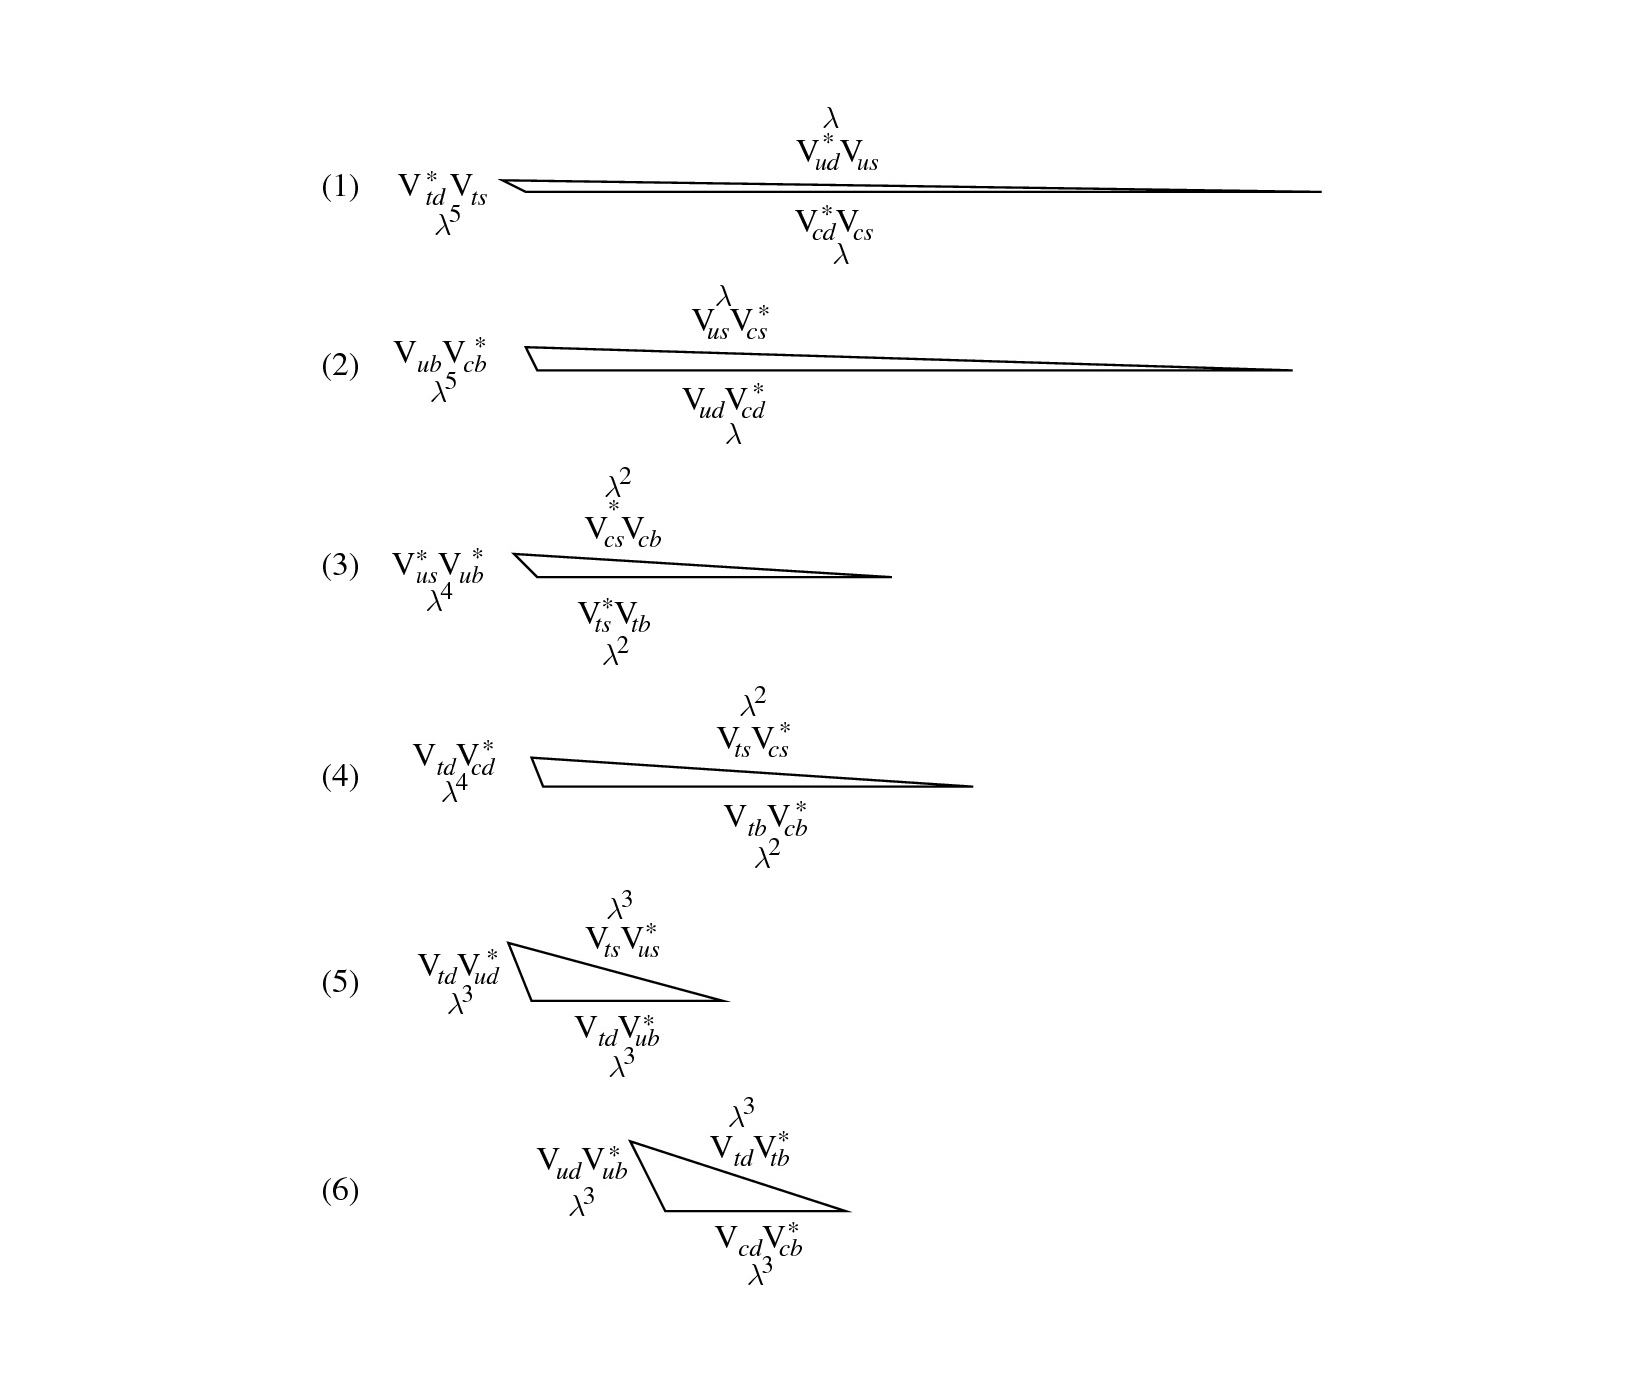
\includegraphics[scale=0.18]{Immagini/triangoli}
\caption{I sei triangoli di unitarietà}
\end{center}
\end{figure}
\section{Triangoli di unitarietà}
\noindent
L'unitarietà della matrice CKM equivale alla validità delle dodici espressioni:
\begin{equation}
  \sum_j V_{ij}V_{jk}^* = \delta_{ik}
\end{equation}
Queste condizioni possono anche essere viste come:
\begin{enumerate}
 \item $6$ relazioni di normalizzazione sulle ampiezze di transizione, cioè la richiesta che la somma dei moduli quadri di tutti gli elementi appartenenti alla stessa riga (colonna) sia pari ad uno:
    \begin{equation}
     \sum_j V_{ij}V_{ji}^* = |V_{ij}|^2 = 1
    \end{equation}
 \item $6$ relazioni di ortogonalità, cioè la richiesta che ogni vettore riga (colonna) sia ortogonale agli altri vettori riga (colonna):
    \begin{equation}
     \sum_j V_{ij}V_{jk}^* = 0 \ \ \ \ \ \ \ \ \ \ \ (i\neq j)
    \end{equation}

\end{enumerate}
Le relazioni di ortogonalità ammettono una immediata interpretazione geometrica: rappresentano infatti sei triangoli nel piano complesso, i cosiddetti \emph{triangoli di unitarietà}.
I lati e gli angoli di questi triangoli non dipendono dalla fase dei campi associati ai quark e sono quindi fisicamente misurabili. Essi rappresentano un ottimo terreno
per testare la validità del Modello Standard, almeno per quanto riguarda le interazioni elettrodeboli. Infatti, se dalla misura dei parametri caratteristici di questi triangoli
sorgessero delle inconsistenze (cioè, ad esempio, se un lato fosse maggiore della somma degli altri due, o se la somma degli angoli interni non fosse pari all'angolo piatto, 
o ancora se i valori degli angoli fossero incompatibili con quelli misurati per i lati, etc...) se ne dedurrebbe che la matrice CKM non è unitaria, con conseguente
crollo del Modello Standard e la scoperta di Nuova Fisica \cite{BigiSanda}.
In seguito si elencheranno i sei triangoli di unitarietà, indicando l'ordine in $\lambda$ di ciascun lato:
\begin{enumerate}
 \item \begin{equation}
\begin{matrix} \underbrace{V_{ud}^*V_{us}}_{O(\lambda)} \end{matrix} \begin{matrix} {+}\\{ } \end{matrix} \begin{matrix} \underbrace{V_{cd}^*V_{cs}}_{O(\lambda)} \end{matrix} \begin{matrix} {+}\\{ } \end{matrix} \begin{matrix} \underbrace{V_{td}^*V_{ts}}_{O(\lambda^5)} \end{matrix} \begin{matrix} {=}\\{ } \end{matrix} \begin{matrix} {0}\\{ } \end{matrix}
 \end{equation}
 \item \begin{equation}
\begin{matrix} \underbrace{V_{ud}V_{cd}^*}_{O(\lambda)} \end{matrix} \begin{matrix} {+}\\{ } \end{matrix} \begin{matrix} \underbrace{V_{us}V_{cs}^*}_{O(\lambda)} \end{matrix} \begin{matrix} {+}\\{ } \end{matrix} \begin{matrix} \underbrace{V_{ub}V_{cb}^*}_{O(\lambda^5)} \end{matrix} \begin{matrix} {=}\\{ } \end{matrix} \begin{matrix} {0}\\{ } \end{matrix}
 \end{equation}
 \item \begin{equation}
\begin{matrix} \underbrace{V_{us}^*V_{ub}}_{O(\lambda^4)} \end{matrix} \begin{matrix} {+}\\{ } \end{matrix} \begin{matrix} \underbrace{V_{cs}^*V_{cb}}_{O(\lambda^2)} \end{matrix} \begin{matrix} {+}\\{ } \end{matrix} \begin{matrix} \underbrace{V_{ts}^*V_{tb}}_{O(\lambda^2)} \end{matrix} \begin{matrix} {=}\\{ } \end{matrix} \begin{matrix} {0}\\{ } \end{matrix}
 \end{equation}
 \item \begin{equation}
\begin{matrix} \underbrace{V_{td}V_{cd}^*}_{O(\lambda^4)} \end{matrix} \begin{matrix} {+}\\{ } \end{matrix} \begin{matrix} \underbrace{V_{ts}V_{cs}^*}_{O(\lambda^2)} \end{matrix} \begin{matrix} {+}\\{ } \end{matrix} \begin{matrix} \underbrace{V_{tb}V_{cb}^*}_{O(\lambda^2)} \end{matrix} \begin{matrix} {=}\\{ } \end{matrix} \begin{matrix} {0}\\{ } \end{matrix}
 \end{equation}
 \item \begin{equation}
\begin{matrix} \underbrace{V_{td}V_{ud}^*}_{O(\lambda^3)} \end{matrix} \begin{matrix} {+}\\{ } \end{matrix} \begin{matrix} \underbrace{V_{ts}V_{us}^*}_{O(\lambda^3)} \end{matrix} \begin{matrix} {+}\\{ } \end{matrix} \begin{matrix} \underbrace{V_{tb}V_{ub}^*}_{O(\lambda^3)} \end{matrix} \begin{matrix} {=}\\{ } \end{matrix} \begin{matrix} {0}\\{ } \end{matrix}
 \end{equation}
 \item \begin{equation}
\begin{matrix} \underbrace{V_{ud}V_{ub}^*}_{O(\lambda^3)} \end{matrix} \begin{matrix} {+}\\{ } \end{matrix} \begin{matrix} \underbrace{V_{cd}V_{cb}^*}_{O(\lambda^3)} \end{matrix} \begin{matrix} {+}\\{ } \end{matrix} \begin{matrix} \underbrace{V_{td}V_{tb}^*}_{O(\lambda^3)} \end{matrix} \begin{matrix} {=}\\{ } \end{matrix} \begin{matrix} {0}\\{ } \end{matrix}
 \end{equation}
\end{enumerate}
Osservando la geometria di questi triangoli, è possibile riunirli in tre diverse categorie:
\begin{enumerate}
 \item I primi due triangoli sono estremamente ``schiacciati``: due lati sono di ordine $\lambda$, metre il terzo di ordine $\lambda^5$, cioè circa $\lambda^4 \approx 2,3 \cdot 10^{-3}$
volte più piccolo. 
 \item Il terzo ed il quarto triangolo sono hanno anch'essi lati di lunghezza molto diseguale, ma non in maniera così marcata.
 \item Gli ultimi due hanno i lati dello stesso ordine di grandezza, ragion per cui i loro angoli sono tutti particolarmente ampi, nell'ordine del radiante.
\end{enumerate}

Nello studio della martice CKM, un particolare interesse ricopre il triangolo dato dall'espressione:
\begin{equation}
 V_{ud}V_{ub}^* + V_{cd}V_{cb}* + V_{td}V_{tb}^* = 0
\end{equation}
A cui spesso ci si riferisce nella letteratura sull'argomento come \emph{il triangolo di unitarietà}, per antonomasia \cite{Branco}.
I parametri attraverso i quali viene definito questo triangolo di unitarietà sono quantità importanti nella dinamica del decadimento del $B$ e nelle oscillazioni $B_d - \bar{B_d}$.
È possibile dimostrare dunque attraverso la matrice CKM che le transizioni deboli che coinvolgono il quark $beauty$ sono dell'ordine dell'unità.
Utilizzando la parametrizzazione di Wolfenstein i lati di questo triangolo risultano essere:
\begin{equation}
V_{ud}V_{ub}^* = -A\lambda^3
\end{equation}
\begin{equation}
V_{cd}V_{cb}* = A\lambda^3 (\bar{\rho} + i\bar{\eta})
\end{equation}
\begin{equation}
 V_{td}V_{tb}^* = A\lambda^3 (1-\bar{\rho}-i\bar{\eta})
\end{equation}
Mentre gli angoli sono:
\begin{equation}
 \alpha = \arg \Big(-\frac{V_{td}V^*_{td}}{V_{ud}V^*_{ub}}\Big)
\end{equation}
\begin{equation}
 \beta = \arg \Big(-\frac{V_{cd}V^*_{cb}}{V_{td}V^*_{tb}}\Big)
\end{equation}
\begin{equation}
 \gamma = \arg\Big(-\frac{V_{ud}V_{ub}^*}{V_{cd}V_{cb}^*}\Big)
\end{equation}
Dato che il seno dell'angolo di Cabibbo $\lambda$ ed il parametro $A$ sono noti con grande precisione, risulta conveniente eseguire una trasformazione di scala
che elimini i fattori $A\lambda^3$, in modo da potersi limitare alla misura di $\rho$ ed $\eta$ \cite{BigiSanda}. Con questa riparametrizzazione uno dei vertici risulta avere coordinate 
$(\bar{\rho},\bar{\eta})$. La misura sperimentale dei parametri esatti di questo triangolo è uno dei problemi aperti più attuali della fisica delle alte energie.
In particolare, nelle parti successive ci si concentrerà sulla misura dell'angolo $\gamma$.
\begin{figure}
\begin{center}
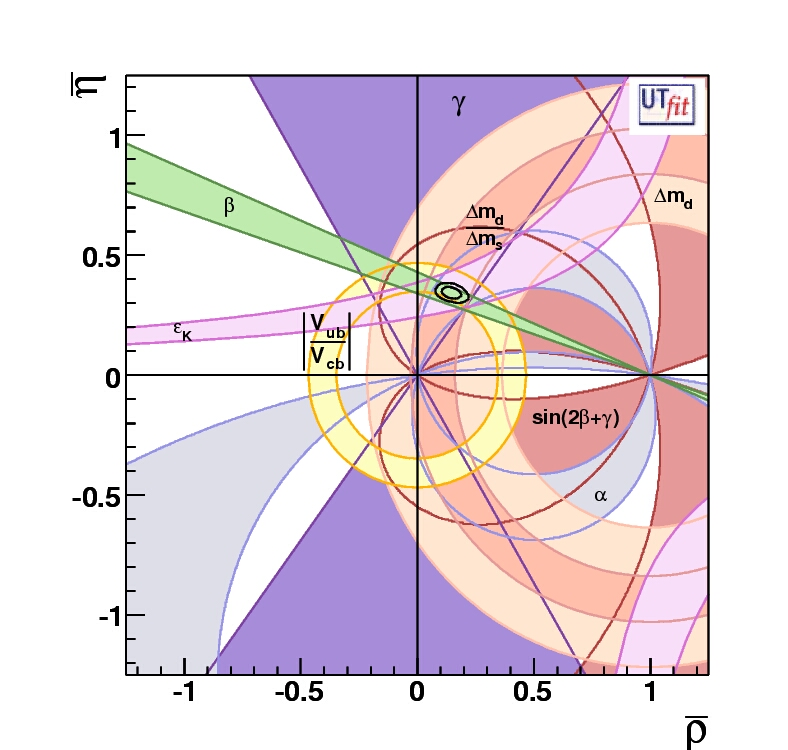
\includegraphics[scale=0.4]{Immagini/triangoloUTfit}
\caption{Lo stato attuale delle misure dei parametri del triangolo di unitarietà. Tutte le misure sono in ottimo accordo con le previsioni teoriche. (\emph{UTfit collaboration, 2012})}
\end{center}
\end{figure}

     %%%%%%%%%%%%%%%%%%%%
     %                  %
     %  capitolo5.tex   %
     %                  %
     %%%%%%%%%%%%%%%%%%%%

\chapter{L' esperimento LHCb}
\noindent
LHCb \`e uno degli esperimenti in corso presso l'acceleratore LHC  del  C.E.R.N. di Ginevra. LHCb ha per obiettivo lo studio della fisica dei quark pesanti \emph{charm} e \emph{beauty}, da realizzare mediante misure di rapporti di diramazione di decadimenti rari e mediante la misura della violazione della simmetria CP in opportuni decadimenti dei mesoni $D$ e $B$ neutri. L'esperimento si propone di evidenziare effetti di Nuova Fisica eventualmente presenti nella dinamica del \emph{flavour} dei quark.

Infatti, sebbene il  meccanismo CKM, descritto nel capitolo precedente, sia sufficiente a dar ragione dei fenomeni di trasformazione del \emph{flavour} e della violazione della simmetria CP osservati con le precisioni attuali, l'entit\`a della violazione di CP prevista da CKM non \`e sufficiente a spiegare l'asimmetria materia-antimateria osservata nell'Universo. Vi sono inoltre modelli teorici che estendono il Modello Standard, i quali prevedono processi addizionali di trasformazione dello stato di \emph{flavour} dei quark, che potrebbero contribuire in misura rilevabile al contributo SM dominante.

L'approccio seguito dall'esperimento LHCb \`e diverso da quello degli altri esperimenti LHC, come ATLAS e CMS: mentre questi ultimi cercano di scoprire effetti di Nuova Fisica attraverso la produzione di nuove particelle, LHCb cerca di misurare eventuali effetti che potrebbero essere prodotti da ampiezze quantistiche dovute a stati virtuali intermedi. Questo approccio ha il grande vantaggio di dare accesso a scale di energia superiori a quelle  richieste per la creazione di stati di particella reali.

Le misure realizzate da LHCb dopo il primo anno di presa dati, con un campione equivalente a circa $1 fb^{-1}$,  sono gi\`a fra le pi\`u precise esistenti al mondo; nel prossimo quinquennio si prevede LHCb possa almeno quintuplicare la dimensione del campione di dati disponibili oggi per le analisi.
 
\begin{figure}
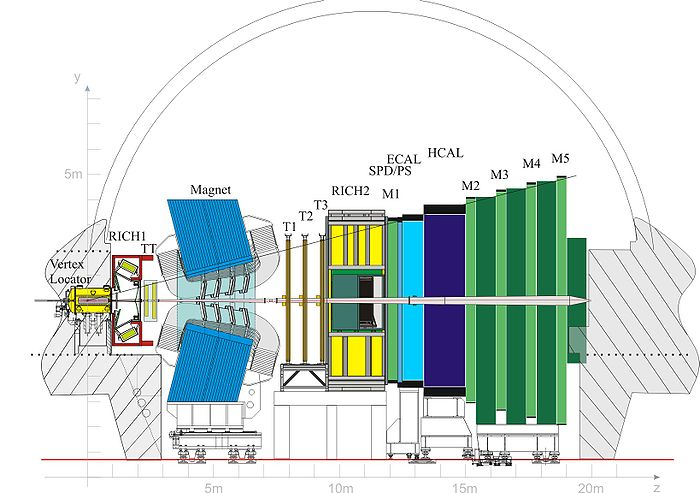
\includegraphics[scale=1]{Immagini/lhcbrivelatore}
\caption{LHCb detector, sezione longitudinale}
\label{fig:detector}
\end{figure}

\section{LHCb detector}
\noindent
Il rivelatore \`e uno spettrometro a singolo braccio, che copre una regione attorno alla linea dei fasci, di estensione angolare compreso tra i $10$ ed i $250$ mrad nel piano verticale e tra i $10$ ed i $300$ mrad nel piano orizzontale. La geometria del rilevatore \`e ottimale per la rivelazione di eventi con produzione di coppie di quark $b\bar{b}$ o $c\bar{c}$, prodotte prevalentemente in avanti e con piccola apertura angolare relativa.

Il rilevatore LHCb \`e costituito da un sistema tracciante per la determinazione delle posizioni dei vertici di produzione e decadimento dei mesoni $B$ e $D$,
per la misura dell'impulso delle tracce cariche, da un calorimetro per la rivelazione dei fotoni, e da un eccellente sistema di identificazione delle particelle. \`E inoltre dotato di un sofisticato sistema di trigger, per l'acquisizione degli eventi d'interesse, in condizioni di elevato fondo. 

\subsection{Sistemi traccianti}
\noindent
Il sistema tracciante consiste di un rivelatore dedicato alla localizzazione dei vertici primari (di collisione protone-protone dei fasci) e dei vertici secondari di decadimento dei mesoni $D$ e $B$, denominato VELO (VErtex LOcator), \`e inoltre costituito da altri quattro rivelatori traccianti (\emph{tracking stations}), posti a distanza dalla regione d' interazione dei fasci, utilizzati per la misura dell'impulso delle particelle.

Per ottenere le risoluzioni richieste i rivelatori sono stati realizzati impiegando \emph{strip} di Silicio. Le regioni pi\`u esterne delle stazioni traccianti collocate dopo il magnete sono state invece realizzate mediante rivelatori a \emph{straw tube}, impiegando cio\`e camere a deriva di forma cilindrica di diametro opportuno.

\subsubsection{Rivelatore di vertice (VELO)}
\noindent
Il VELO \`e il sistema di localizzazione dei vertici primari e secondari che consente di misurare la loro posizione con una risoluzione spaziale di circa $10\ \mu m$. 
 Si consideri che la lunghezza di volo dei mesoni $B$ da misurare, alle energie (\emph{boost}) di LHC, risulta essere in media dell'ordine del centimetro. 
Il VELO  \`e costituito da ventiquattro moduli di rivelazione, collocati attorno alla regione d'interazione, disposti in sequenza, perpendicolarmente alla linea definita dai fasci, in modo da coprire una regione di estensione complessiva di circa un metro. Ciascun modulo serve per misurare le coordinate radiale ed angolare dei segnali prodotti dalle particelle cariche che attraversano il rilevatore (\emph{hit}). A partire dalla misura delle \emph{hit} in prossimit\`a della regione d'interazione dei fasci, \`e possibile ricostruire con grande precisione la geometria delle traiettorie delle particelle cariche e localizzare con precisione i vertici primari e secondari. 
\begin{figure}[h]
\centering
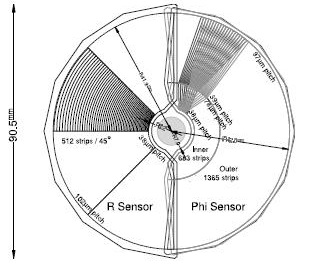
\includegraphics[scale=1]{Immagini/velo1}
\caption{Schema di uno dei ventiquattro moduli che costituiscono il rivelatore di vertice VELO di LHCb. La figura illustra la geometria dei sensori in silicio impiegati per la misura delle coordinate radiale ed angolare delle \emph{hit}.}
\label{fig:velo2}
\end{figure}
%
\subsubsection{Camere traccianti (per la misura dell'impulso).}
\noindent
Il sistema di tracciamento impiegato per la misura dell'impulso delle particelle \`e costituito dal \emph{Trigger Tracker}, posto a monte del magnete, e da tre stazioni \emph{Tracking Stations}, indicate con le sigle $T1$, $T2$ e $T3$, poste a valle di esso, come indicato in Figura \ref{fig:detector}. Ognuno di queste stazioni traccianti \`e costituta da quattro piani di rivelazione indipendenti, impiegati per una misura ridondante e bidimensionale delle \emph{hit } prodotte dalle particelle cariche che attraversano il rivelatore. 

Il sistema tracciante copre una superficie ortogonale alla traiettoria dei fasci pari a $150 × 130$ $cm^2$, corrispondente all'intero angolo solido di accettanza del detector.
\begin{figure}
\centering
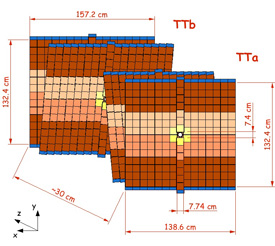
\includegraphics[scale=0.9]{Immagini/TriggerTracker}
\caption{Il sistema di tracciamento Trigger Tracker. Sono visibili i diversi settori, a diversa segmentazione, e nella parte esterna, in blu, 
i circuiti di lettura \emph{readout hybrids}.}
\label{fig:TriggerTracker}
\end{figure}
La parte pi\`u interna delle stazioni traccianti (\emph{Inner Tracker}, IT) \`e costituita da sensori al silicio, simili a quelli usati per il \emph{Trigger Tracker}, con una
differente disposizione dei sensori e segmentazione dei moduli, per le diverse esigenze di risoluzione spaziale a maggiore distanza. 
La regione esterna (\emph{Outer Tracker}, OT) \`e stata realizzata sovrapponendo quattro piani di tubi a deriva, del diametro di $5$ mm, riempiti da una miscela gassosa costituita per il $70\%$ di argon e per il $30\%$ di diossido di carbonio. La miscela permette di avere un tempo di deriva inferiore ai $50$ ns, adeguato per l'elevata frequenza di conteggio  (gli eventi si sussegguono ogni $25$ ns con occupanze medie inferiori al 10\%).
%
%
\subsection{Sistemi di identificazione delle particelle}
\noindent
Il sistema di identificazione si basa sull'uso di due rilevatori di luce Cherenkov RICH (RICH1 e RICH2), su due calorimetri ECAL ed HCAL e sul rivelatore di muoni.
\subsubsection{RICH}
\noindent
\begin{figure}
\centering
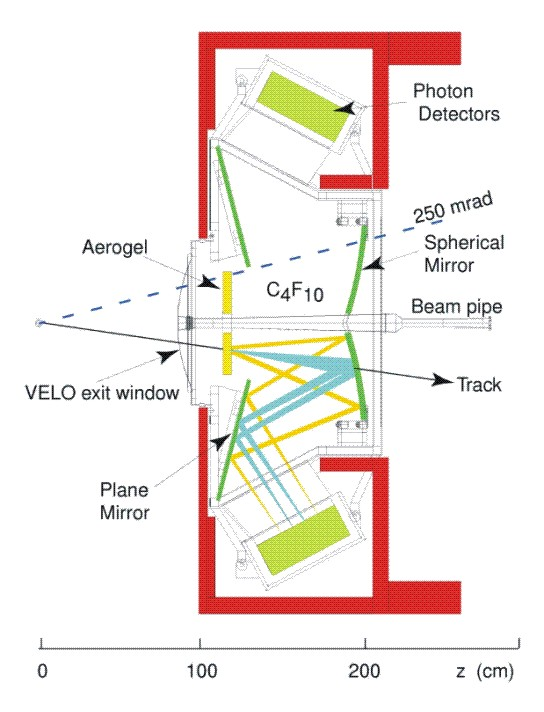
\includegraphics[scale=1.5]{Immagini/rich}
\caption{Rivelatore RICH1}
\label{fig:rich}
\end{figure}
Il riconoscimento delle particelle mediante i RICH si basa sulla misura dell'angolo Cherenkov, noto il valore dell'impulso della traccia corrispondente.

I due rivelatori RICH di LHCb (in Figura \ref{fig:rich} \`e mostrato soltanto uno di essi) sono essenziali per il riconoscimento dei decadimenti dei mesoni $D$ e $B$ in stati finali adronici. Essi permettono di distinguere le tracce dovute a pioni, kaoni e protoni che attraversano il rilevatore, in un intervallo d'impulso compreso tra $10$ ed $100$ GeV/c.

Il rivelatore RICH1 \`e posto in prossimit\`a della regione di interazione e copre per intero l'accettanza geometrica di LHCb. \`E dedicato alla rivelazione delle tracce con impulso fra $10\div60$ GeV/c. 
RICH2 \`e posto a distanza maggiore dalla regione di interazione, oltre l'ultima delle \emph{Tracking Stations}, in modo da intercettare le particelle  nell'intervallo d'impulso maggiore,  compreso tra $20$ e $100$ GeV/c. Copre una regione di angolo solido poco estesa, prossima alla linea dei fasci.

Il rilevatore RICH1 impiega due diversi mezzi radiatori: per identificare le particelle con impulso minore \`e utilizzato aerogel, un composto colloidale del quarzo, il cui indice di rifrazione \`e compreso tra $1,01$ e $1,10$; per identificare le particelle di impulso maggiore \`e utilizzato fluorobutano ($C_4F_{10}$) con indice di rifrazione $1,0014$.
Nel RICH2 \`e utilizzato tetrafluorometano ($CF_4$), con indice di rifrazione pari a $1.00048$, per rivelare le particelle della parte superiore dello spettro. La figura di merito \`e mostrata in Figura \ref{fig:rich2}
\begin{figure}
\centering
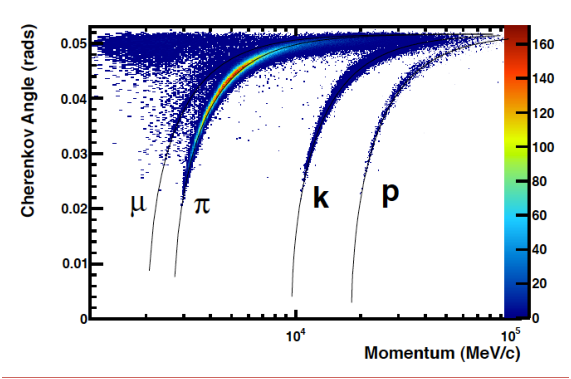
\includegraphics[scale=1.2]{Immagini/PastedGraphic-2}
\caption{Angolo di Cherenkov in funzione del mezzo radiatore e dell'impulso della particella che lo attraversa}
\label{fig:rich2}
\end{figure}

\subsubsection{Calorimetri}
\noindent
Il calorimetro adronico HCAL non \`e utilizzato \emph{offline} per l'analisi, \`e utilizzato solo in fase di trigger, per individuare eventi con adroni di elevato impulso trasversale.  
Il calorimetro elettromagnetico ECAL (con l'aggiunta di rivelatori ausiliari SPD, PS) \`e impiegato anche offline per la identificazione di fotoni, elettroni e pioni neutri.
SPD (\emph{Scintillator Pad Detector}) e PS (\emph{Preshower Detector}) forniscono segnali ausiliari ad ECAL per la discriminazione carico/neutro e la reiezione dei segnali adronici.
\begin{figure}[b]
\centering
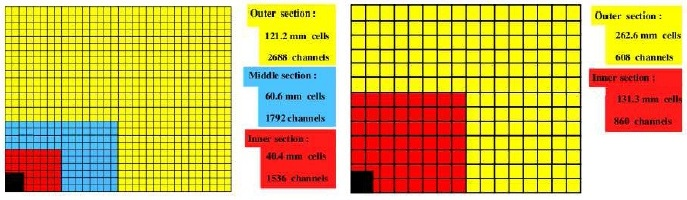
\includegraphics[scale=0.65]{Immagini/ECAL}
\caption{Schema dei calorimetri impiegati in LHCb. A destra ECAL, PS e SPD, a sinistra HCAL}
\label{fig:ECAL}
\end{figure}
ECAL \`e un calorimetro a campionamento, formato da piani assorbitori in piombo intervallati a piani sensibili di scintillatori. Analogamente HCAL \`e un calorimetro a campionamento, costituito per\`o da lastre di ferro, intervallate a scintillatori plastici. I segnali di scintillazione sono letti in entrambe i casi mediante fibre ottiche che convogliano i segnali a fotomoltiplicatori.

I calorimetri permettono di distinguere $e^\pm$ da $\pi^\pm$ con una efficienza del $90\%$ e un livello di contaminazione inferiore all'$1\%$.
La risoluzione in energia del calorimetro elettromagnetico \`e dell'ordine di qualche percento nel \emph{range} di impulso compreso tra $10$ e $100$ $GeV/c$.

\subsubsection{Rilevatore di muoni}
\begin{figure}
\centering
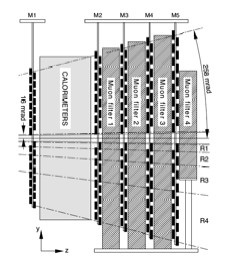
\includegraphics[scale=1]{Immagini/muon}
\caption{Rilevatore di muoni. Sono visibili le cinque camere impiegate per la rilevazione, indicate con le sigle $M_2$, $M_3$, $M_4$ ed $M_5$}
\label{fig:muon}
\end{figure}
\noindent
Poiché parte considerevole dei canali di decadimento dei mesoni $B$ e $D$ contengono muoni, la loro corretta identificazione \`e di cruciale importanza.
Il sistema di rivelazione dei muoni \`e impiega cinque stazioni di rivelazione ($M_1$, $M_2$, $M_3$, $M_4$ ed $M_5$) realizzate utilizzando camere traccianti MWPC (\emph{MultiWire Proportional Chamber}). Il sistema di rivelazione intercetta il $20\%$ dei muoni prodotti dai vari canali di decadimento del $B$ con un efficienza superiore al 95\%.
La stazione $M_1$, collocata prima dei calorimetri, deve sostenere un flusso di particelle superiore alle altre, e per questo motivo, nella regione prossima ai fasci, \`e stata  equipaggiata con rivelatori che sostengono alti rate di conteggio di tipo GEM (\emph{Gas Electron Multiplier}). Le camere $M_2$, $M_3$, $M_4$ ed $M_5$, per rivelare i muoni penetranti (perch\'e un muone superi tutte le stazioni traccianti deve avere un'energia superiore a $10$ $GeV$), sono pertanto intervallate a lastre di ferro spesse $80$ cm. Le camere traccianti hanno una risoluzione temporale inferiore a $25$ ns.

\section{Aquisizione dei dati}
\noindent
La frequenza di collisioni rivelate da LHCb \`e dell'ordine dei $10$ MHz, molto superiore alla frequenza di segnale, dell'ordine di qualche $kHz$.
Per questo motivo LHCb \`e stato dotato di un sistema di \emph{trigger} che consente di ridurre la frequenza di registrazione degli eventi a 5 $kHz$.

Il sistema di \emph{trigger} \`e strutturato su due livelli: il primo livello, chiamato L0, opera alla frequenza di \emph{bunch crossing} di LHC di $40$ MHz;
  il secondo livello, chiamato HLT (\emph{Hig Level Trigger}) opera in cascata alla frequenza di $1$ MHz.

Il trigger L0 selezione eventi con particelle di elevato impulso trasversale, mentre il trigger HLT  seleziona  eventi specifici per mezzo di algoritmi in esecuzione, in parallelo, su un \emph{cluster} di computer, costituito da alcune decine di migliaia di CPU.

Gli eventi raccolti sono inviati al centro di calcolo TIer-0 del CERN che oltre alla elaborazione di parte di essi, distribuisce i dati a sei centri di calcolo europei $Tier-1$. Fra 
i centri di calcolo vi \`e centro nazionale dell'INFN presso il CNAF di Bologna. I centri di calcolo sono utilizzati per l'elaborazione preliminare dei dati e successivamente per l'analisi utente. La produzione di eventi di simulazione \`e realizzata presso centri dedicati denominati Tier2.


     %%%%%%%%%%%%%%%%%%%%
     %                  %
     %  capitolo6.tex   %
     %                  %
     %%%%%%%%%%%%%%%%%%%%

\chapter{Combinazione di misure dell'angolo $\gamma$}
\noindent
In questo capitolo si illustreranno i tre principali metodi impiegati per la valutazione di $\gamma$, chiamati \emph{GLW} (Gronau-London-Wyler, \cite{Gronau:1990ra}\cite{Gronau:1991dp}), 
\emph{ADS} (Atwood-Dunietz-Soni, \cite{Atwood:1996ci}) e \emph{GGSZ} (Giri-Grossman-Soffer-Zupan, \cite{Giri:2003ty}) 
\begin{figure}
\begin{center}
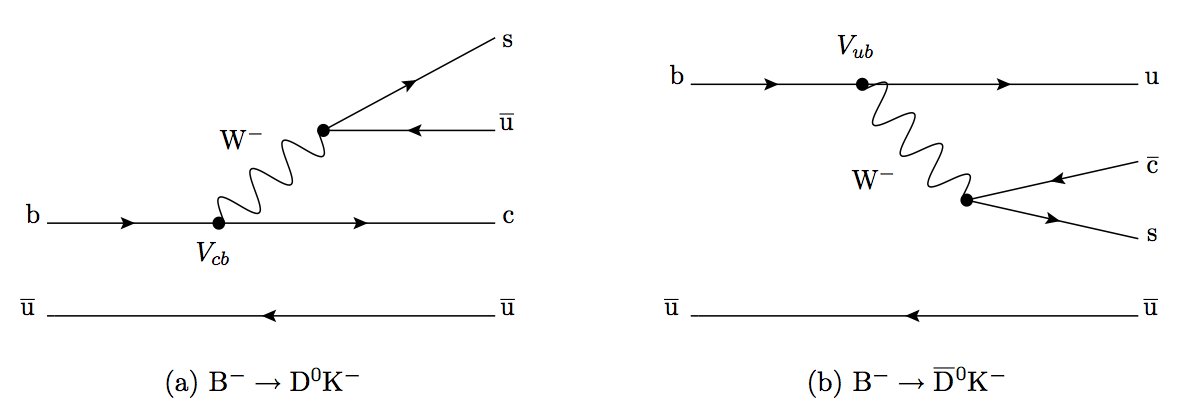
\includegraphics[scale=0.3]{Immagini/diagrammi}
\caption{Decadimenti $B^{-} \longrightarrow D[\rightarrow f]K^{-}$ studiati per misurare il valore dell'angolo $\gamma$}
\label{DIAGRAMMIDIFEYNMAN}
\end{center}
\end{figure}

La misura di $\gamma$ si basa sullo studio delle interferenze dei decadimenti $b\rightarrow u$ e $b\rightarrow c$ in processi ad albero del tipo:
\begin{equation}\label{B-dec}
 B^{-} \longrightarrow D[\rightarrow f]K^{-}
\end{equation}
nei quali $D$ può indicare sia il $D^0$ che a il $\bar{D^0}$ (Fig. \ref{DIAGRAMMIDIFEYNMAN}). 
Le interferenze tra le diverse ampiezze di decadimento dipendono dalla fase debole $\gamma$.

I tre metodi menzionati differiscono tra loro per i diversi stati finali di $D$  usati nell'analisi:
\begin{enumerate}
 \item \emph{GLW}: analizza i decadimenti nei quali gli stati finali del $D$ sono CP-coniugati (ad esempio $D\rightarrow \pi\pi$).
 \item \emph{ADS}: si basa sui decadimenti \emph{Cabibbo favoriti} (CF) (ad esempio $B^-\rightarrow D^0[\rightarrow K^{-}\pi^{+}] K^-$) e \emph{doppiamente Cabibbo soppressi} (DCS) (ad esempio $B^-\rightarrow D[\rightarrow K^{+}\pi^{-}] K^-$).
 \item \emph{GGSZ}:analizza i decadimenti C-coniugati in tre corpi (ad esempio $D\rightarrow K_S K^\pm K^\mp$). 
                   Per misuare le osservabili dipendenti da $\gamma$ è necessario eseguire un'analisi di Dalitz.
\end{enumerate}
La migliore precisione su $\gamma$ si ottiene combinando i risultati di tutte queste analisi. 

Di seguito sono definiti alcuni parametri che risulteranno utili nella trattazione successiva:
\begin{enumerate}
 \item $r$: rapporto fra le ampiezze di decadimento DCS e CF del $B$ e del $D$;
 \item $\delta$: differenza di fase forte;
 \item Le ampiezze di decadimento del $B^-$ e del $D$ possono essere scritte nel seguente modo:
\begin{displaymath}
\left\{
\begin{array}{l}
A(B^- \rightarrow DK^-) = A_ce^{i\delta_c}\\
A(B^- \rightarrow \bar{D}K^-) = A_ue^{i\delta_u-\gamma}\\
A(D \rightarrow f) = A_fe^{i\delta_f}\\
A(D \rightarrow \bar{f}) = A_ce^{i\delta_{\bar{f}}}
\end{array}
\right.
\end{displaymath}
dove $A_c$, $A_u$, $A_f$ e $A_{\bar{f}}$ sono grandezze reali e positive. Si è ignorata la violazione di CP nel decadimento del $D$ (si noti l'assenza del termine $\gamma$
nei decadimenti di quest'ultimo). Gli indici $u$ e $c$ si riferiscono rispettivamente alle transizioni $b\rightarrow u$ e $b\rightarrow c$.
Qualora il $D^0$ segua un canale di decadimento in tre corpi, le quantità $A_f$, $A_{\bar{f}}$, $\delta_f$ e $\delta_{\bar{f}}$ saranno funzioni delle coordinate nel diagramma
di Dalitz.
\end{enumerate} 
L'ampiezza del decadimento $B^- \rightarrow D[\rightarrow f]K^-)$ è data dall'equazione:
\begin{equation}
 A (B^-\rightarrow D[\rightarrow f]K^-) = A_cA_fe^{i(\delta_c + \delta_f)} + A_u A_fe^{i\delta_u + \delta_{\bar{f}} - \gamma}
\end{equation}
Da cui si deduce la seguente espressione per il tasso di decadimento:
\begin{equation}\label{probability}
 \Gamma (B^-\rightarrow D[\rightarrow f]K^-) \propto A_c^2\big(A_f^2 + r_B^2A_{\bar{f}}^2 + 2r_BA_fA_{\bar{f}}\cos(\delta_B + \delta_D - \gamma)\big)
\end{equation}
con $r_B = A_u/A_c$, $\delta_B = \delta_u - \delta_c$ e $\delta_D = \delta_{\bar{f}} - \delta_f$.

Nei paragrafi successivi verrà descritta l'analisi che permette di combinare le recenti misure di LHCb nei decadimento $B^{\pm}\rightarrow DK^{\pm}$ 
\cite{LHCBB2}\cite{LHCBB3}\cite{LHCBB4} per estrarre, 
mediante un metodo basato sulla statistica di Bayes, gli intervalli di credibilità dell'angolo $\gamma$ e dei parametri di interesse associati. Le analisi sono 
realizzate con i dati raccolti da LHCb nel 2011, corrispondenti ad una luminosità integrata di $1$ $fb^{-1}$, nelle collisioni $p$-$p$ ad LHC.  Nei seguenti paragrafi,
verranno brevemente descritti i metodi GLW, ADS e GGSZ, il metodo di estrazione di gamma mediante la statistica bayesiana ed infine verranno discussi i risultati. 


\section{Metodo GLW}
\noindent
Nell'analisi GLW, si studiano decadimenti ad albero i cui prodotti finali sono autostati di CP, ad esempio:
\begin{equation}
 D\longrightarrow K^-K^+\ \ \ \ \ \ \ \ \ \ \ \ \ \ \ \ (CP = +1)
\end{equation}
\begin{equation}
 D\longrightarrow K_s\pi^0\ \ \ \ \ \ \ \ \ \ \ \ \ \ \ \ \ \ (CP = -1)
\end{equation}
Per cui si ha ${A_f}/A_{\bar{f}} = 1$ e $\delta_D = 0, \pi$. Pertanto l'equazione \eqref{probability} diventa:
\begin{equation}\label{numera}
 \Gamma(B^- \rightarrow D^0[\rightarrow f_{CP=\pm1}]K^-) \propto A_c^2 (1 + r_B^2 \pm 2r_B\cos(\delta_B - \gamma))
\end{equation}
Per normalizzare questa espressione possono essere usati i decadimenti ad albero $B^-\rightarrow D^0[\rightarrow K^{-}\pi^{+}] K^-$ e $B^-\rightarrow \bar{D^0}[\rightarrow K^{+}\pi^{-}] K^-$ 
, nei quali cioè il $D^0$ decade secondo i canali CF. Si può scrivere, con buona approssimazione:
\begin{equation}\label{normalizzazione}
 \Gamma(B^-\rightarrow D^0[\rightarrow K^-\pi^+]K^-) =  \Gamma(B^-\rightarrow \bar{D}^0[\rightarrow K^+\pi^-]K^-) = \propto A_c^2
\end{equation}
A questo punto è possibile definire gli osservabili $R_{CP\pm}$ e $A_{CP\pm}$ nel modo seguente:
\begin{equation}\label{RCP}
 R_{CP\pm} = \frac{2[\Gamma(B^- \rightarrow D_{CP\pm}^0K^-) + \Gamma(B^+\rightarrow D_{CP\pm}^0K^+)]}{\Gamma (B^-\rightarrow D^0K^-) + \Gamma (B^+ \rightarrow \bar{D}^0K^+)} = 1 + r_B^2 \pm 2r_B \cos \delta_B \cos \gamma
\end{equation}
\begin{equation}\label{ACP}
 A_{CP\pm} = \frac{\Gamma(B^- \rightarrow D_{CP\pm}^0K^-) - \Gamma(B^+\rightarrow D_{CP\pm}^0K^+)}{\Gamma(B^- \rightarrow D_{CP\pm}^0K^-) + \Gamma(B^+\rightarrow D_{CP\pm}^0K^+)} = \frac{\pm 2r_B\sin\delta_B\sin\gamma}{R_{CP\pm}}
\end{equation}
Le due equazioni \eqref{RCP} e \eqref{ACP} forniscono un sistema di quattro equazioni nelle tre incognite $\gamma$, $r_B$ e $\delta_B$, 
quindi una misura di $R_{CP\pm}$ e di $A_{CP\pm}$ permette di ottenere una misura di queste tre quantità. 
Lo stato sperimentale di queste misure è riportato in Tab. \ref{tab:Acp}.

\begin{table}
  \begin{center}
    \begin{small}
      \begin{tabular}{|c|c|c|c|c|}

\hline
 & \textbf{$A_{CP+}$} & \textbf{$A_{CP-}$} & \textbf{$R_{CP+}$} & \textbf{$R_{CP-}$}\\
\hline
\textbf{BaBar} & $0.25 \pm 0.06 \pm 0.02$ & $-0.09 \pm 0.07 \pm 0.02$  & $1.18 \pm 0.09 \pm 0.05$ & $1.07 \pm 0.08 \pm 0.04$\\
\hline
\textbf{Belle} & $0.29 \pm 0.06 \pm 0.02$ & $-0.12 \pm 0.06 \pm 0.01$ & $1.03 \pm 0.07 \pm 0.03$& $1.13 \pm 0.09 \pm 0.05$\\
\hline
\textbf{CDF} & $0.39 \pm 0.17 \pm 0.04$ & - & $1.30 \pm 0.24 \pm 0.12$ & -\\
\hline
\textbf{LHCb} & $0.14 \pm 0.03 \pm 0.01$ & - & $1.01 \pm 0.04 \pm 0.01$ & -\\
\hline
\textbf{Media} & $0.19 \pm 0.03$ & $-0.11 \pm 0.05$ & $1.03 \pm 0.03$ & $1.10 \pm 0.07$\\
\hline
      \end{tabular}
    \end{small}
  \end{center}
\caption{Stato sperimentale attuale (2012) delle misure dei parametri $A_{CP+}$, $A_{CP-}$, $R_{CP+}$ e $R_{CP-}$. I valori medi sono quelli ottenuti dalla collaborazione
         HFAG\cite{HFAG}.}
\label{tab:Acp}

\end{table}


\section{Metodo ADS}
\noindent
Nell'analisi ADS, vengono selezionati i canali di decadimento CF (ad esempio $B\rightarrow D^0[\rightarrow K^{-}\pi^{+}] K^-$) e 
DCS (ad esempio $B\rightarrow D^0[\rightarrow K^{+}\pi^{-}] K^-$).

Il tasso di decadimento sensibile a $\gamma$ è il risultato dell'interferenza del canale favorito dal punto di vista del colore $B^-\rightarrow D^0K^-$ seguito dal processo
doppiamente Cabibbo soppresso $D^0\rightarrow \pi^-K^+$ e dal canale sfavorito da punto di vista del colore $B^-\rightarrow \bar{D^0}K^-$ seguito dal canale
Cabibbo favorito $D^0\rightarrow K^-\pi^+$. Le ampiezze in gioco sono di grandezza simile, per cui gli effetti di interferenza tra le due sono di notevole intensità.
A partire dall'equazione \eqref{probability} si dimostra che:
\begin{equation} \label{GLWgamma}
 \Gamma(B^{\mp}\rightarrow D^0[\rightarrow K^{\pm}\pi^{\mp}]K^{\mp}) \propto r_B^2 + r_D^2 \pm 2r_Br_D \cos(\delta_B + \delta_D \mp \gamma)
\end{equation}
dove $r_B = A_f/A_{\bar{f}} = |A(D^0 \rightarrow \pi^-K^+)/A(D^0\rightarrow K^-\pi^+)|$ e $\delta_D$ è la differenza di fase forte tra i due decadimenti. $r_D$ e $\delta_D$
entrano nell'analisi come parametri noti, il cui valore può essere determinato usando i dati raccolti dalla collaborazione Cleo nelle collisioni elettrone-positrone alla 
risonanza $\psi(3770)$ \cite{cleo}. È possibile ora definire le quantità $R_{ADS}$ e $A_{ADS}$:
\begin{equation}
 R_{ADS} = \frac{\Gamma(B^- \rightarrow D^0[\rightarrow \pi^- K^+]K^-) + \Gamma(B^+ \rightarrow D^0[\rightarrow \pi^+K^-]K^+)}{\Gamma(B^- \rightarrow D^0[\rightarrow K^- \pi^+]K^-) + \Gamma(B^+ \rightarrow D^0[\rightarrow K^+\pi^-]K^+)}
\end{equation}
\begin{equation}
 A_{ADS} = \frac{\Gamma(B^- \rightarrow D^0[\rightarrow \pi^- K^+]K^-) - \Gamma(B^+ \rightarrow D^0[\rightarrow \pi^+K^-]K^+)}{\Gamma(B^- \rightarrow D^0[\rightarrow K^- \pi^+]K^-) + \Gamma(B^+ \rightarrow D^0[\rightarrow \pi^+K^-]K^+)}
\end{equation}
Sostituendo in queste espressioni le equazioni \eqref{normalizzazione} e \eqref{GLWgamma} si ottiene:
\begin{equation}
 R_{ADS} = r_B^2 + r_{K\pi}^2 + 2r_Br_{K\pi}\cos\gamma\cos(\delta_B + \delta_{D})
\end{equation}
\begin{equation}
 A_{ADS} = \frac {2r_B r_{K\pi}\sin\gamma\sin(\delta_B + \delta_{D})}{R_{ADS}}
\end{equation}
Queste due quantità hanno lo svantaggio di essere correlate. È possibile definire le due variabili scorrelate $R_\pm$:
\begin{equation}
 R_{\pm} = \frac{\Gamma(B^{\pm}\rightarrow D^0[\rightarrow K^{\mp}\pi^{\pm})]K^{\mp})}{\Gamma(B^{\pm}\rightarrow D^0[\rightarrow K^{\pm}\pi^{\mp}]K^{\pm})} = \frac{1}{N}(r_B^2 + r_{K\pi}^2 + 2r_Br_{K\pi}\cos(\delta_B + \delta_{K\pi} \pm \gamma)) 
\end{equation}
dove $N$ è una costante vicina ad uno. Queste due nuove quantità sono statisticamente indipendenti.
\begin{table}
\begin{center}
\begin{tabular}{|c|c|c|}\hline
 & \textbf{$A_{ADS}$} & \textbf{$R_{ADS}$}\\\hline
\textbf{BaBar} & $-0.86 \pm 0.47_{-0.16}^{+0.12}$ & $0.011 \pm 0.006 \pm 0.002$\\\hline
\textbf{Belle} & $-0.39_{-0.28 -0.03}^{+0.26 +0.04}$ & $0.0163_{- 0.0041 - 0.0013}^{+0.0044 + 0.0007}$\\\hline
\textbf{CDF} & $-0.82 \pm 0.44 \pm 0.09$ & $0.0220 \pm 0.0086 \pm 0.0026$\\\hline
\textbf{LHCb} & $-0.52 \pm 0.15 \pm 0.02$ & $0.0152 \pm 0.0020 \pm 0.0004$\\\hline
\textbf{Media} & $-0.54 \pm 0.12$ & $0.0153 \pm 0.0017$\\\hline
\end{tabular}
\end{center}
\caption{Stato attuale (2012) delle misure sperimentali di $A_{ADS}$ e $R_{ADS}$. I valori medi sono quelli ottenuti dalla collaborazione
         HFAG\cite{HFAG}.}
\label{referenzatabella}
\end{table}
Lo stato sperimentale delle grandezze $A_{ADS}$ e $R_{ADS}$ è riportato in Tab. \ref{referenzatabella}. 


\section{Metodo GGSZ}
\noindent
Nell'analisi GGSZ, vengono studiati i decadimenti in tre corpi C-coniugati del $D$:
\begin{equation}\label{decadimento}
 D \rightarrow K_S\pi^+\pi^- \ \ \ \ \ \ \ \ \ \ \ \ \ \ \ \ D \rightarrow K_SK^+K^-
\end{equation}
Le ampiezze sono $A_fe^{i\delta_f} = f(m_-^2, m_+^2)$ e $A_{\bar{f}}e^{i\delta_{\bar{f}}} = f(m_+^2, m_-^2)$
dove si è indicata con $m_+$ la massa del sistema $K_S\pi^+(K^+)$ e con $m_-$ quella di $K_S\pi^-(K^-)$.
I tassi di decadimento possono essere scritti come:
\begin{equation}\label{GGSZ}
 \Gamma(B^{\mp} \rightarrow D[\rightarrow K_Sh^+h^-)]K^{\mp}) \propto  
\end{equation}
\begin{equation*}
 \propto |f(m_{\mp}^2, m_{\pm}^2)|^2 + r_B^2|f(m_{\pm}^2, m_{\mp}^2)|^2 + 2r_B|f(m_{\mp}^2 + m_{\pm}^2)||f(m_{\mp}^2, m_{\pm}^2)\cos(\delta_B + \delta_D(m_{\mp}^2, m_{\pm}^2)\mp \gamma)
\end{equation*}
dove $h$ può indicare un $\pi$ o un $K$, mentre $\delta_D(m_{\mp}^2, m_{\pm}^2)$ è la differenza di fase forte tra $f(m_{\pm}^2, m_{\mp}^2)$ e $f(m_{\mp}^2, m_{\pm}^2)$.

Introducendo le \emph{coordinate cartesiane}, definite come:
\begin{equation}
 x_{\pm} = \Re [r_Be^{i(\delta_B \pm \gamma)}]
\end{equation}
\begin{equation}
 y_{\pm} = \Im [r_Be^{i(\delta_B \pm \gamma)}]
\end{equation}
è possibile riscrivere la \eqref{GGSZ} come:
\begin{equation}
\Gamma(B^{\mp} \rightarrow D^0[\rightarrow K_S\pi^+\pi^-)]K^{\mp}) \propto |f_{\mp}|^2 + r_B^2|f_{\pm}|^2 + 2[x_{\mp}\Re[f_{\mp}f_{\pm^*}] + y_{\mp} \Im[f_{\mp}f_{\pm}]] 
\end{equation}
dove sono state usate le notazioni compatte $f_{\pm} = f(m_{\pm}^2, m_{\mp}^2)$ e $f_{\mp} = f(m_{\mp}^2, m_{\pm}^2)$.
\begin{table}
\begin{center}
\footnotesize
\begin{tabular}{|c|c|c|c|c|}\hline
 & \textbf{BaBar} & \textbf{Belle} & \textbf{Media} & \textbf{LHCb}\\\hline
$x_+$ & $-0.103\pm0.037\pm0.006\pm0.007$ & $-0.107\pm0.043\pm0.011\pm0.055$ & $-0.104\pm0.029$ & $-0.1030 \pm 0.0504$\\\hline
$y_+$ & $-0.021\pm0.048\pm0.004\pm0.009$ & $-0.067\pm0.059\pm0.018\pm0.063$ & $0.085\pm0.030$ & $-0.009 \pm0.048$\\\hline
$x_-$ & $0.060\pm0.039\pm0.007\pm0.006$ & $0.105\pm0.047\pm0.018\pm0.063$ & $0.085\pm0.030$ & $0.000 \pm0.0459$ \\\hline
$y_-$ & $0.062\pm0.045\pm0.004\pm0.006$ & $0.177\pm0.060\pm0.018\pm0.054$ & $0.105\pm0.036$ & $0.0270 \pm 0.0574$\\\hline
\end{tabular}
\normalsize
\end{center}
\caption{Stato attuale (2012) delle misure dei parametri $x_\pm$ e $y_\pm$. I valori medi sono quelli ottenuti dalla collaborazione
         HFAG\cite{HFAG}.}
\label{xy}
\end{table}
I valori sperimentali di $x_\pm$ e $y_\pm$ sono riportati in Tab. \ref{xy}.

\section{Statistica Bayesiana}
\noindent
Nei paragrafi precedenti è stato descritto come sia possibile misurare, attraverso lo studio dei decadimenti $B^\pm \rightarrow D^0K^\pm$,
alcune osservabili che sono funzioni dell'angolo $\gamma$. Per combinare tutte le osservabili ed ottenere un'unica misura di $\gamma$ sarà usata l'\emph{analisi statistica 
bayesiana}.
Di seguito è riportato l'enunciato teorema di Bayes, con una semplice dimostrazione.

\begin{teorema}
 Si consideri un gruppo completo di ipotesi incompatibili, dette $H_1$, $H_2$, $...$ , $H_n$. Si esegue ora un esperimento che porta al verificarsi dell'evento $A$.
Allora, la probabilità che $A$ sia stato causato dalla validità dell'ipotesi $H_i$ è data da:
\begin{equation}
 P(H_i|A) = \frac{P(H_i)P(A|H_i)}{\sum_{i = 1}^n P(H_i)P(A|H_i)}
\end{equation}
\end{teorema}
\begin{proof}
 In accordo con la regola di moltiplicazione delle probabilità si ha:
\begin{equation}
 P(AH_i) = P(A|H_i)P(H_i) = P(H_i|A)P(A)
\end{equation}
Risolvendo rispetto a $P(H_i|A)$ si ottiene:
\begin{equation}\label{PHiA}
P(H_i|A) = \frac{P(H_i)P(A|H_i)}{P(A)}
\end{equation}
Ma la probabilità che si verifichi $A$ è data dalla somma sulle $n$ ipotesi $H_n$ dei prodotti $P(A|H_i)P(H_i)$:
\begin{equation}\label{PA}
P(A) = \sum_{i = 1}^n P(H_i)P(A|H_i) 
\end{equation}
Per cui, sostituendo la \eqref{PA} nella \eqref{PHiA} si ottiene la tesi.
\end{proof}
L'ovvia generalizzazione al caso continuo di quanto esposto è:
\begin{equation}
 f(H|A) = \frac{f(H)f(A|H)}{\int f(H)f(A|H)dH}
\end{equation}
Le grandezze che compaiono in questa formula non sono più probabilità discrete ma densità di probabilità \cite{d'agostini}. Esse sono definite nel modo seguente:
\begin{enumerate}
 \item $f(A|H)$, cioè la probabilità di registrare un certo valore sperimentale $A$ data l'ipotesi $H$, è detta anche \emph{verosimiglianza}
 \item $f(H)$, cioè la probabilità di validità dell'ipotesi $H$, detta anche probabilità \emph{a priori} o \emph{prior}. In mancanza di informazioni ulteriori che rendano alcune 
       ipotesi più probabili di altre viene si assume che abbia lo stesso valore su ogni $H$. 
 \item $f(H|A)$, cioè la probabilità di validità dell'ipotesi $H$ una volta registrato il dato sperimentale $A$. Viene anche detta probabilità \emph{a posteriori}.
\end{enumerate}
Nel caso più generale $H$ ed $A$ sono grandezze vettoriali:
\begin{equation}
  f(\vec{H}|\vec{A}) = \frac{f(\vec{H})f(\vec{A}|\vec{H})}{\int f(\vec{H})f(\vec{A}|\vec{H})d\vec{H}}
\end{equation}
Nell'analisi svolta in questa tesi si ha:
\begin{enumerate}
 \item $\vec{H} = (\gamma, r_B, \delta_B, r_D, \delta_D)$
 \item $\vec{A} = (R_{CP+}, A_{CP+}, R_+, R_-, x_\pm, y_\pm)$
\end{enumerate}
Per ottenere la misura di $\gamma$ è necessario conoscere la densità di probabilità \emph{a posteriori} $f(\vec{H}|\vec{A})$ in maniera da ottenere da questa la densità
di probabilità di $\gamma$, $f(\gamma)$, secondo la formula:
\begin{equation}
 f(\gamma) = \int f(\vec{H}|\vec{A}) dr_Bd\delta_Bdr_Dd\delta_D
\end{equation}
Uno strumento di calcolo utile a questo scopo è il \emph{framework} BAT, che verrà descritto nel seguente paragrafo.

\section{BAT (\emph{Bayesian Analysis Toolkit})}
\noindent
Per determinare la distribuzione di probabilità \emph{a posteriori} $f(\vec{H}|\vec{A})$ si è utilizzato il \emph{framework} BAT.
Esso implementa alcuni algoritmi utili a realizzare l'analisi bayesiana dei dati.
Lo scopo  è quello di dare risposta a due esigenze:
\begin{enumerate}
 \item fornire uno strumento flessibile che permetta la formulazione di ogni tipo di modello
 \item fornire un codice di analisi numerica fortemente ottimizzato che permetta la gestione di una grande quantità di operazioni
\end{enumerate}
È scritto in C++ e si basa su ROOT per le funzioni di input/output e realizzazione di grafici.
Le sue funzioni includono la mappatura della probabilità a posteriori in uno spazio dei parametri multidimensionale,
la stima dei parametri e dei relativi intervalli di credibilità, il calcolo della correlazione tra diversi parametri, etc.
Il cuore centrale di BAT è costituito da \emph{Metropolis}, un algoritmo che implementa il metodo MCMC (\emph{Markov Chain Monte Carlo}) e che verrà discusso dettagliatamente nel seguito.
\subsection{Markov Chain Monte Carlo}
\noindent
Ottenere la probabilità \emph{a posteriori} è solitamente un problema molto difficile, specialmente nel caso di un modello con un alto numero di parametri.
In particolare, risulta particolarmente dispendioso dal punto di vista del calcolo trovare il fattore di normalizzazione $\int f(\vec{H})f(\vec{A}|\vec{H})d\vec{H}$.
Per ovviare a questa difficoltà vengono largamente impiegati metodi numerici, in modo particolare il metodo MCMC, che permette di estrarre numeri casuali secondo 
la distribuzione statistica $f(\vec{H})f(\vec{A}|\vec{H})/\int f(\vec{H})f(\vec{A}|\vec{H})d\vec{H}$ senza conoscere il fattore di 
normalizzazione $\int f(\vec{H})f(\vec{A}|\vec{H})d\vec{H}$, cioè ammettendo come unica ipotesi di poter confrontare la distribuzione in due punti arbitrari 
$\vec{H_i}$ ed $\vec{H_j}$ calcolando il rapporto $\frac{f(\vec{H_i})f(\vec{A}|\vec{H_i})}{f(\vec{H_j})f(\vec{A}|\vec{H_j})}$.
 
Come indica il nome, si tratta di un processo di Markov, per cui ogni valore $f(\vec{H_i})f(\vec{A}|\vec{H_i})$ calcolato con questa tecnica risulta correlato 
al precedente $f(\vec{H_{i-1}})f(\vec{A}|\vec{H_{i-1}})$ ed indipendente da tutti gli altri.
L'algoritmo che lo implementa all'interno di BAT, \emph{Metropolis}, consta di quattro passi:
\begin{enumerate}
 \item Si sceglie un punto $\vec{H_i}$ nello spazio dei parametri, la cui dimensionalità dipenderà dal tipo di problema studiato
 \item Si sceglie in maniera casuale un secondo punto $H'$, usando una distribuzione statistica a simmetria sferica centrata in $H_i$, 
       $g_{H_i}(H_i')$ (solitamente si tratta di una distribuzione uniforme in un dato intorno di $H_i$ e nulla al di fuori).
 \item Si calcolano $f(\vec{H_i})f(\vec{A}|\vec{H_i})$ e $f(\vec{H'})f(\vec{A}|\vec{H'})$.
       Se $f(\vec{H'})f(\vec{A}|\vec{H'}) \geq f(\vec{H_i})f(\vec{A}|\vec{H_i})$ si pone $H_{i+1} = H'$. 
       Se $f(\vec{H'})f(\vec{A}|\vec{H'}) \leq f(\vec{H_i})f(\vec{A}|\vec{H_i})$ il valore di $H_{i+1}$ verrà scelto in maniera aleatoria:
       si avrà $H_{i+1} = H'$ con probabilità pari a $\frac{f(\vec{H'})f(\vec{A}|\vec{H'})}{f(\vec{H_i})f(\vec{A}|\vec{H_i})}$, altrimenti $H_{i+1} = H_i$ (con, ovviamente, probabilità pari a $1-\frac{f(\vec{H'})f(\vec{A}|\vec{H'})}{f(\vec{H_i})f(\vec{A}|\vec{H_i})}$).
 \item A questo punto il ciclo viene iterato a partire dal secondo passo.
\end{enumerate}
È ragionevole supporre che, dopo un certo numero di cicli, l'istogramma normalizzato delle $H_i$ campionate darà un'approssimazione sufficientemente accurata della 
distribuzione $f(\vec{H}|\vec{A})$. Si può anche procedere in maniera formale e dimostrare che la catena di Markov impiegata nel procedimento ammette come 
distribuzione di equilibrio la funzione $f(\vec{H}|\vec{A})$ ricercata, ma la discussione è al di là del livello di questa tesi, per cui non verrà qui affrontata.

\section{Osservabili e metodo di misura}
\noindent
Come già accennato la misura di $\gamma$ verrà effettuata calcolando grazie a BAT la seguente densità di probabilità:
\begin{equation}
   f(\vec{H}|\vec{A}) = \frac{f(\vec{H})f\vec{A}|\vec{H})}{\int f(\vec{H})f(\vec{A}|\vec{H})d\vec{H}}
\end{equation}
Dove $f(\vec{H})$ è la distribuzione statistica \emph{a priori}, data dal prodotto delle cinque distribuzioni \emph{a priori} delle incognite del problema ($\gamma$, $r_B$, $\delta_B$, $r_D$ e $\delta_D$).
Poiché la combinazione eseguita vuole essere indipendente dalle misure precedenti di $\gamma$, $r_B$ e $\delta_B$;
le distribuzioni \emph{a priori} di queste grandezze vengono poste costanti.
Per $r_D$ e $\delta_D$, al contrario, si scelgono come \emph{prior} delle gaussiane centrate sui valori 
delle due grandezze forniti dalla collaborazione Cleo e di deviazione standard pari all'incertezza sperimentale sugli stessi.
Infatti il sistema non ha sensibilità sufficiente a gestire una distribuzione piatta anche su queste grandezze per cui, se non si inserisse su queste un'informazione
esterna (cioè la misura di Cleo), ne risulterebbe un valore di $\gamma$ completamente indeterminato.

\begin{table}
\begin{center}
\begin{tabular}{|c|c|}
\hline
\textbf{Osservabile} & \textbf{Distribuzione a priori}\\\hline
$\gamma$ & $\chi[0 , 180]$\\\hline
$\delta_B$ & $\chi[0,180]$\\\hline
$r_B$ & $\chi[0, 0.3]$\\\hline
$\delta_D$ & $G(-152, 10)$\\\hline
$r_D$ & $G(0.00376, 0.00009)$\\\hline
\end{tabular}
\end{center}
\caption{Si è indicata con $\chi[a,b]$, $a,b \in \mathbb{R}$ la funzione caratteristica dell'intervallo $[a,b]$ (normalizzata in maniera tale da avere integrale unitario sul dominio), 
mentre con $G(\bar{x}, \sigma)$ ($\bar{x}, \sigma \in \mathbb{R}$) si è indicata la funzione di Gauss (anch'essa normalizzata ad uno) di media $\bar{x}$ e deviazione standard $\sigma$.}
\label{tabellaprior}
\end{table}
I cinque \emph{prior} sono elencati brevemente in Tab. \ref{tabellaprior}.
La verosimiglienza $f(\vec{A}|\vec{H})$ è data dalla formula seguente:
\begin{equation}
 f(\vec{A}|\vec{H}) = \prod_i \exp-\left(\frac{(A_i(\vec{H}) - O_i)^2}{2\sigma_{O_i}}\right)
\end{equation}
dove con $O_i$ è stato indicato il valore misurato dell'$i$-esimo osservabile, con $\sigma_{O_i}$ la sua incertezza e con $c_i(\alpha)$ la sua espressione come funzione delle
incognite, ricavata attraverso i tre metodi GLW, ADS e GGSZ discussi in precedenza.
In Tab.\ref{O_i} sono riportati i valori $O_i$ e $\sigma_{O_i}$ relativi a ciascuna osservabile, nonché l'espressione della stessa in funzione delle incognite. 
\begin{table}
\begin{center}
\begin{tabular}{|c|c|c|c|}\hline
\textbf{Osservabile} & \textbf{$O_i$} & \textbf{$\sigma_{O_i}$} & \textbf{$A_i$}\\\hline
$R_{CP^+}$ & $1.01$ & $0.04$ & $1 + r_B^2 + 2r_B \cos \delta_B \cos \gamma$\\\hline 
$A_{CP^+}$ & $0.14$ & $0.03$ & $\frac{ 2r_B\sin\delta_B\sin\gamma}{R_{CP+}}$\\\hline
$R_+$ & $0.0232$ & $0.0034$ & $\frac{1}{N}(r_B^2 + r_{D}^2 + 2r_Br_{D}\cos(\delta_B + \delta_{D} + \gamma))$\\\hline
$R_-$ & $0.0073$ & $0.0023$ & $\frac{1}{N}(r_B^2 + r_{D}^2 + 2r_Br_{D}\cos(\delta_B + \delta_{D} - \gamma))$\\\hline
$x_+$ & $0.0 \cdot 10^{-2}$ & $4.6\cdot 10^{-2}$ & $r_B\cos(\delta_B + \gamma)$\\\hline
$x_-$ & $2.7\cdot 10^{-2}$ & $5.7\cdot 10^{-2}$ & $r_B\cos(\delta_B - \gamma)$\\\hline
$y_+$ & $-10.3\cdot 10^{-2}$ & $5.0\cdot 10^{-2}$ & $r_B\sin(\delta_B +\gamma)$\\\hline
$y_-$ & $-0.9\cdot 10^{-2}$ & $4.8\cdot 10^{-2}$ & $r_B\sin(\delta_B -\gamma)$\\\hline
\end{tabular}
\end{center}
\caption{Le osservabili impiegate per il calcolo di $\gamma$. Di ciascuna viene indicato il valore misurato da LHCb, l'incertezza sperimentale e l'espressione in funzione di $\gamma$, $r_B$ e $\delta_B$}
\label{O_i}
\end{table}
\section{Risultati}
\noindent
Le figure \ref{grafici} mostrano le distribuzioni di probabilità a posteriori rispettivamente per i parametri $\gamma$, $\delta_B$ e $r_B$. Esistono diversi metodi per calcolare 
l'intervallo di credibilità, per questo lavoro di tesi è stato usato quello più diffuso nell'ambito della statistica di Bayes. Esso consiste nel determinare 
l'intervallo più piccolo con la più alta densità di probabilità e nel quale è contenuto il valore più probabile. In questo modo è possibile determinare gli intervalli
di credibilità corrispondenti al $68\%$ e $95\%$  della probabilità totale. I valori così ottenuti sono riportati in Tab. \ref{risultati}. 
Le figure \ref{grafici} e \ref{correlazione} mostrano rispettivamente i grafici di $\gamma$, $\delta_B$, $r_B$ e le distribuzioni \emph{a posteriori} bidimensionali delle coppie di grandezze $(\gamma, \delta_B)$, $(\delta_B, r_B)$ e $(\gamma, r_B)$.

Il risultato finale per gamma è:

\begin{equation}
 \gamma = (60.3^{+17.1}_{-13.5})^{\circ}
\end{equation}
 
Questo risultato è in ottimo accordo con le recenti misure già ottenute dalle Collaborazioni BaBar\cite{BaBar} e Belle\cite{Belle}: $\gamma_{BaBar} = 69^{+17}_{-16}$ e $ \gamma_{Belle} =  68^{+15}_{-14}$.
LHCb ha quindi un enorme potenziale sulla misura di $\gamma$, considerando che l'analisi condotta in questa tesi è stata realizzata con il $40\%$ della statistica totale raccolta da LHCb ad oggi (LHCb ha infatti raccolto 2.5 $fb^{-1}$).

\begin{table}
\begin{center}
\begin{tabular}{|c|c|c|c|}\hline
\textbf{Parametro} & \textbf{\textit{Valore più probabile}} & \textbf{$68\%$} & \textbf{$95\%$}\\\hline
$\gamma$ & $60.3$ & $[46.8, 77.4]$ &  $[32.4,102.6]$   \\\hline
$r_B$ & $0.0885$ & $[0.078, 0.102]$ &  $[0.066,0.111]$   \\\hline
$\delta_B$ & $103.5$ & $[88.2, 122.4]$ &  $[68.4,138.6]$ \\\hline
\end{tabular}
\caption{Risultati dell'analisi per $r_B$, $\delta_B$ e $\gamma$. Per ciascuna di esse viene specificato il valore più probabile (la moda della distribuzione), l'intervallo di confidenza
 al $68\%$ e quello al $95\%$. }
\label{risultati}
\end{center}
\end{table}
\begin{figure}[htbp] 
\begin{center}
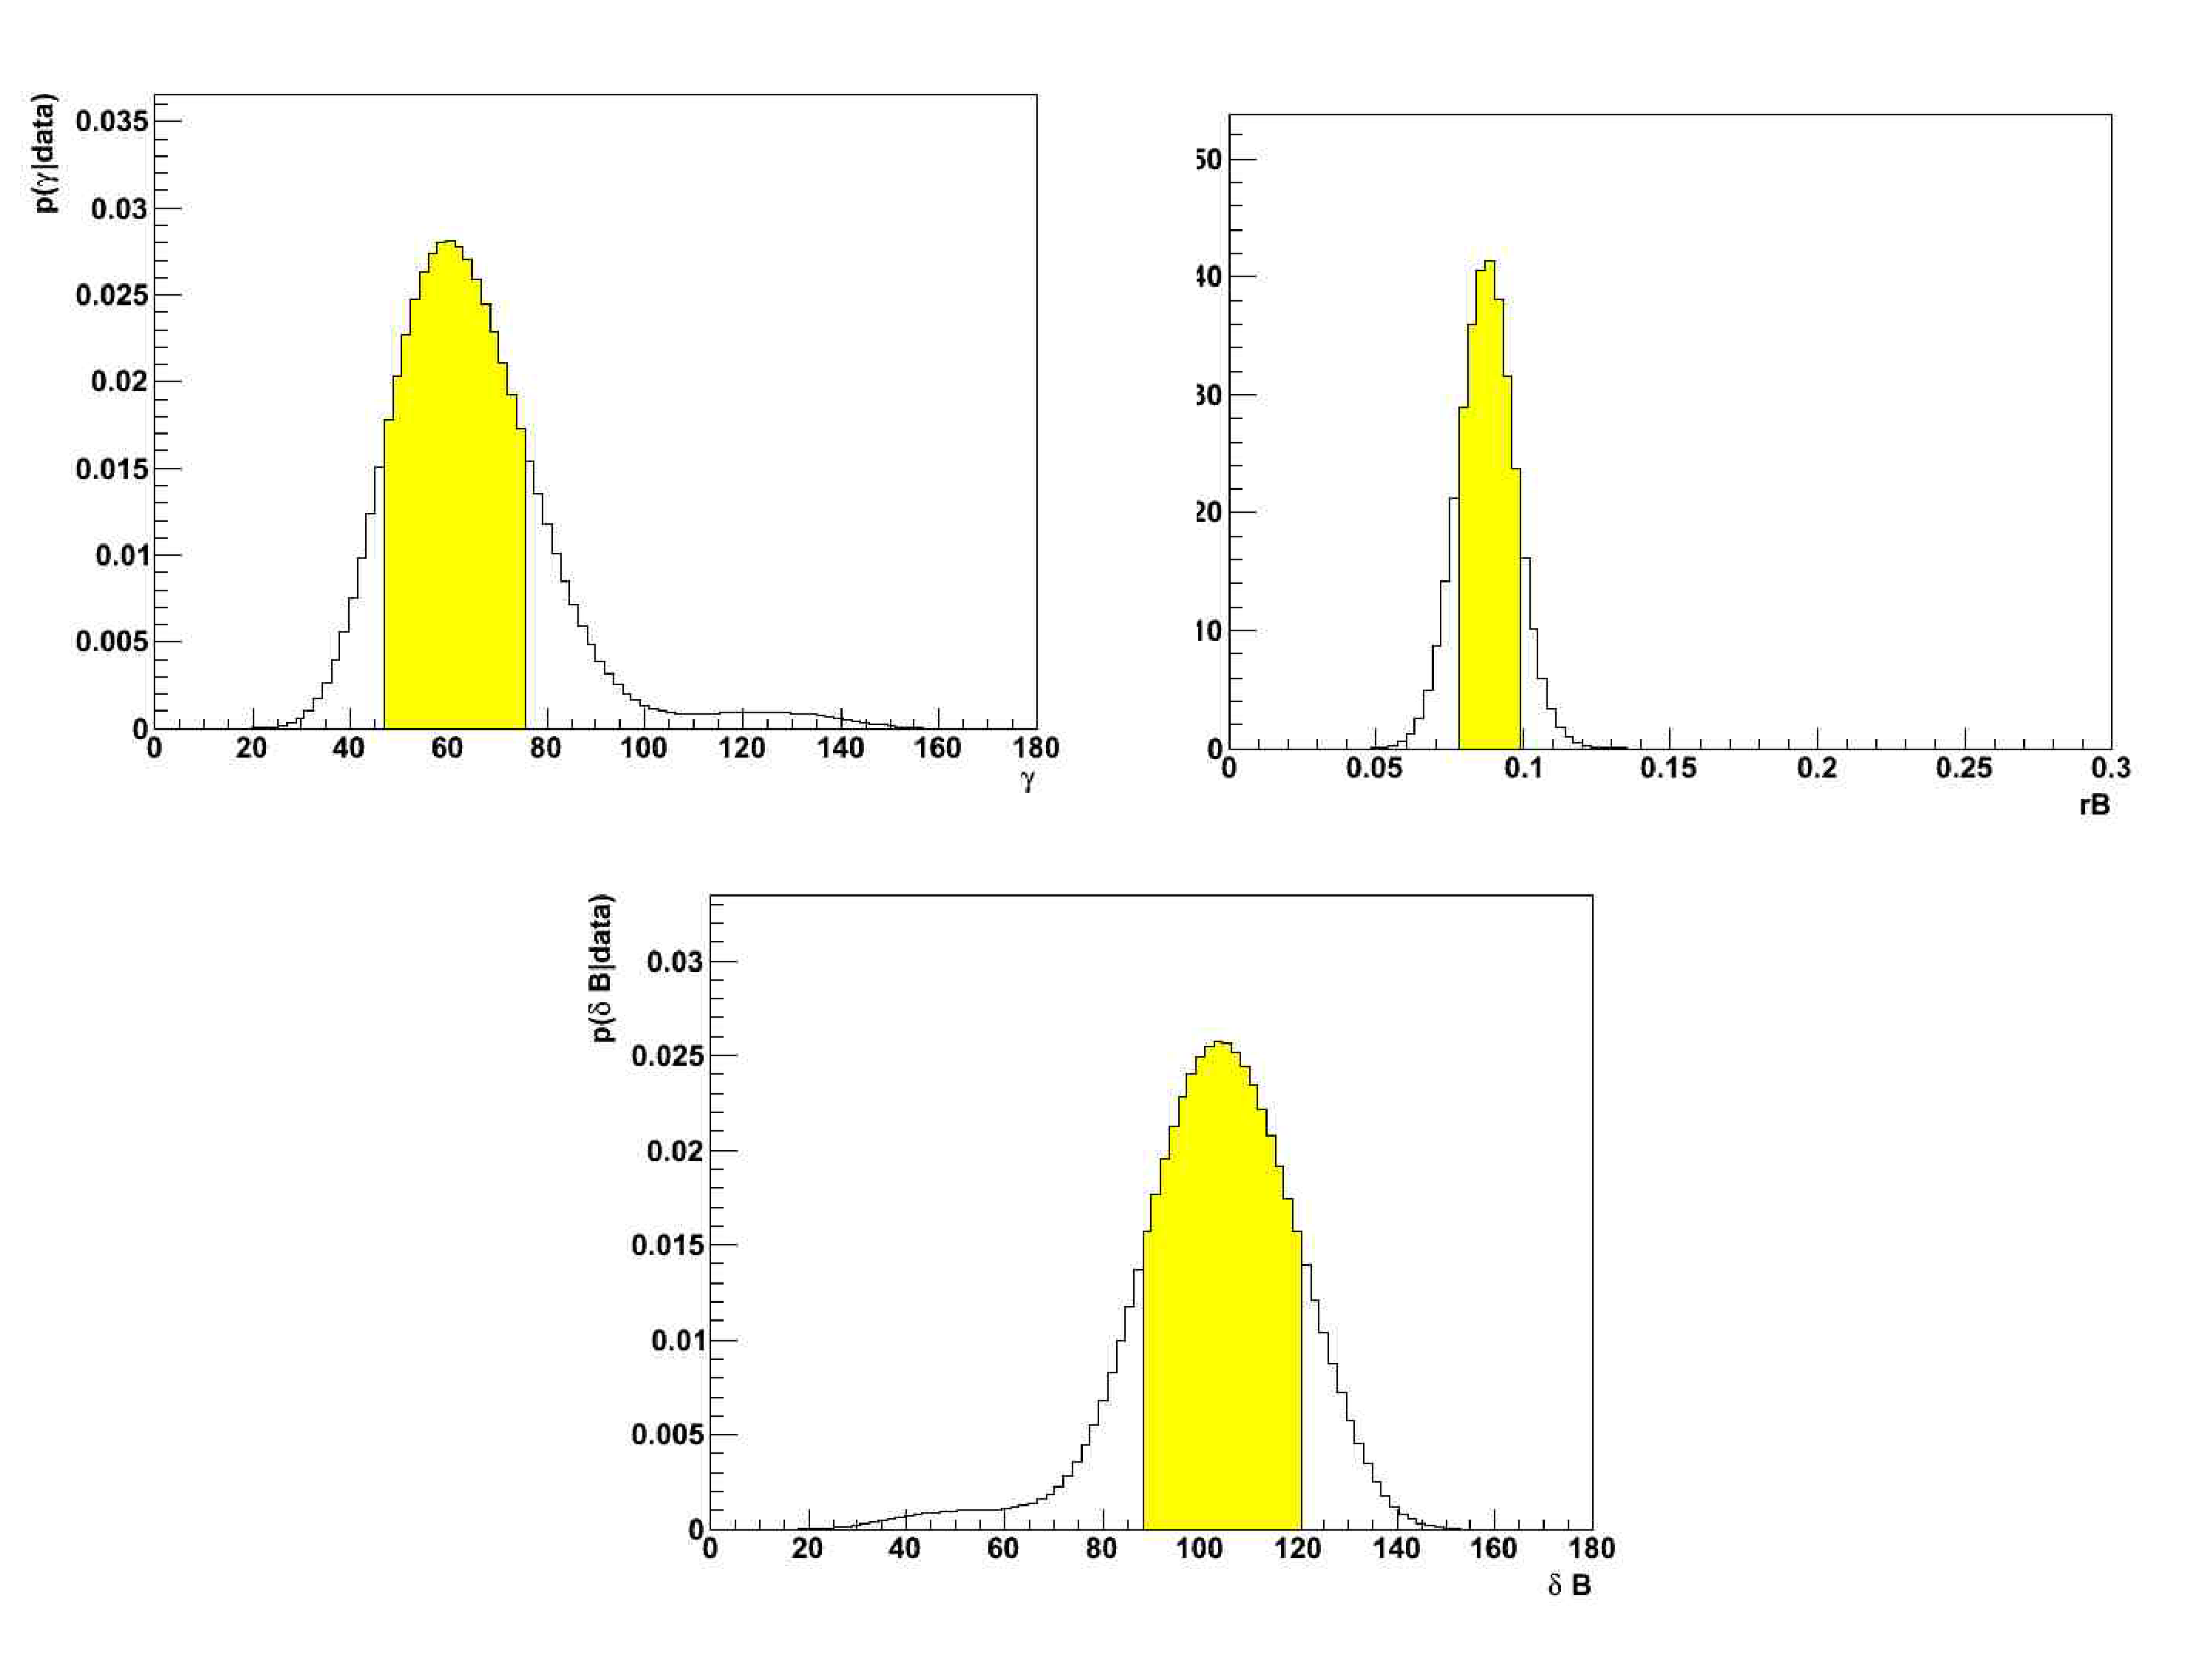
\includegraphics[width=1\textwidth]{Immagini/Plot}
\caption{Distribuzioni di probabilità \emph{a posteriori} di $\gamma$ (in alto a sinistra), $r_B$ (in alto a destra) e $\delta_B$ (in basso). L'area evidenziata in giallo rappresenta il più piccolo intevallo con la più alta densità di probabilità corrispondente al $68\%$ dell'area totale. }
\label{grafici}
\end{center}
\end{figure}

\begin{figure}[htbp] 
\begin{center}
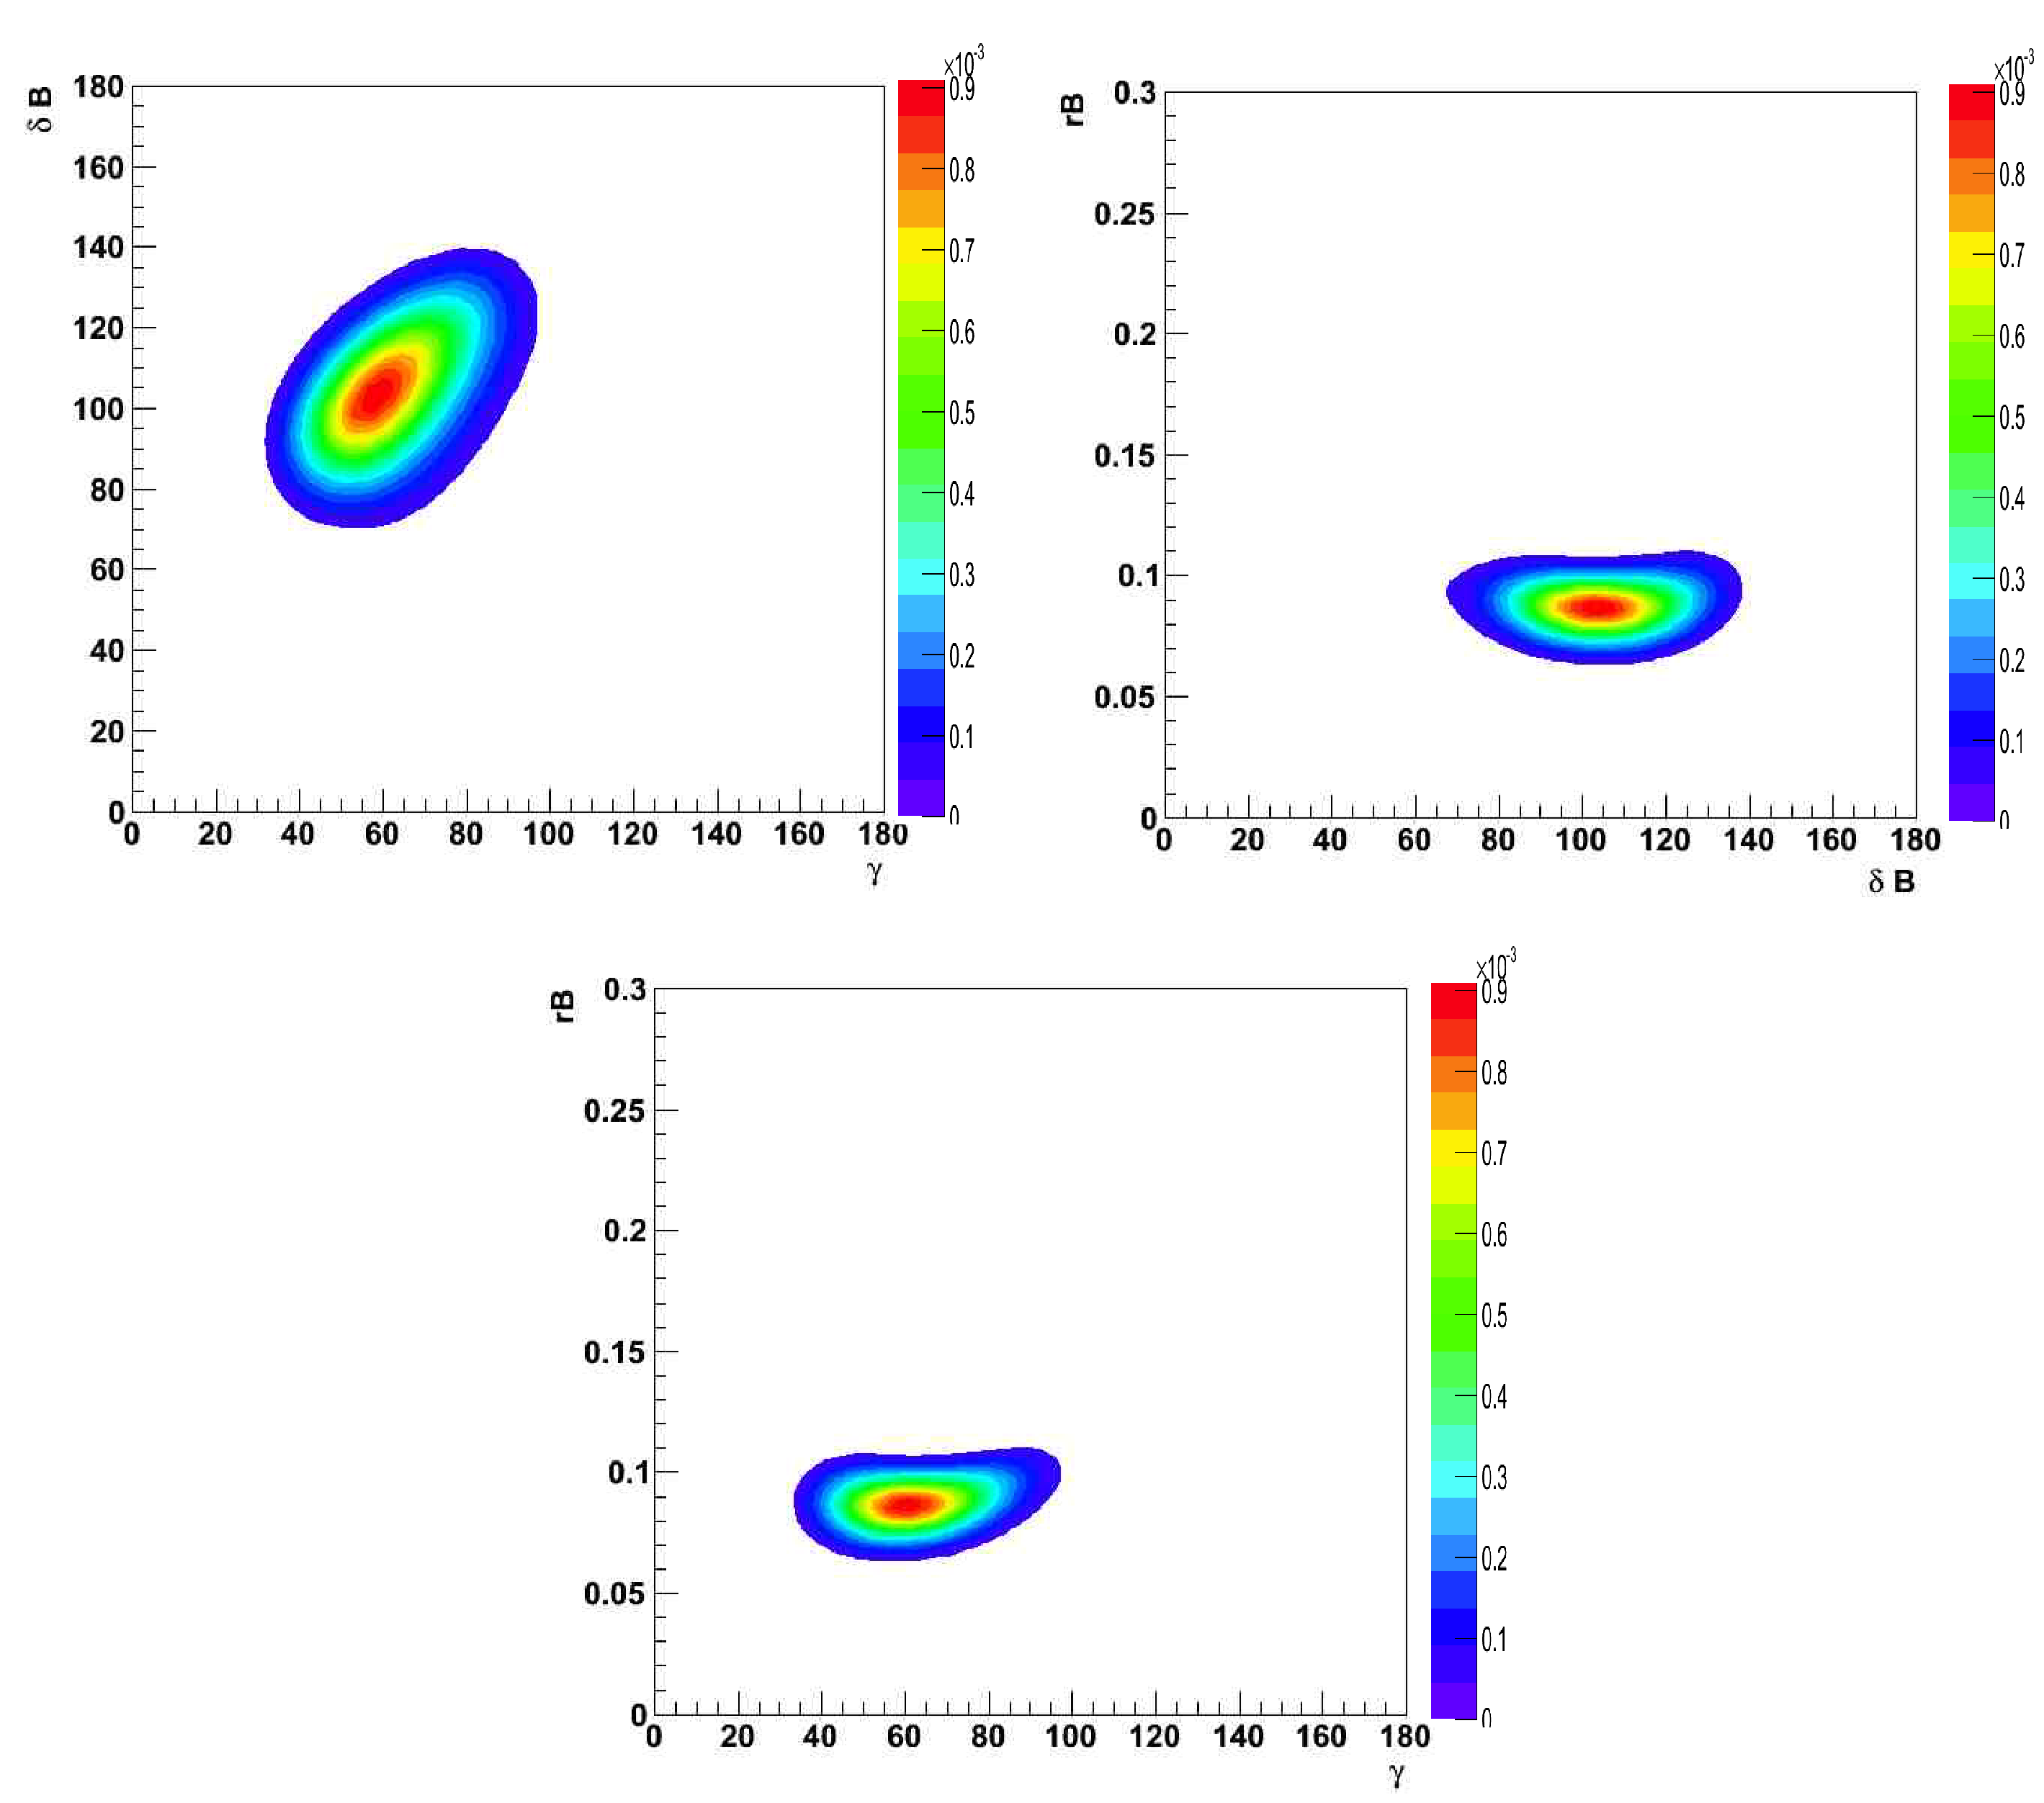
\includegraphics[width=1\textwidth]{Immagini/correlazione}
\caption{Distribuzioni \emph{a posteriori} bidimensionali delle coppie di grandezze $(\gamma, \delta_B)$ (in alto a sinistra), $(\delta_B, r_B)$(in alto a destra) e $(\gamma, r_B)$ (in basso).}
\label{correlazione}
\end{center}
\end{figure}




\renewcommand{\theequation}{\arabic{equation}}%consigliato per migliorare i numeri di equazione nell'introduzione
\renewcommand{\thesection}{\arabic{section}}%consigliato per migliorare i numeri di equazione nell'introduzione
     %%%%%%%%%%%%%%%%%%%%
     %                  %
     %  conclusioni.tex %
     %                  %
     %%%%%%%%%%%%%%%%%%%%

\chapter*{Conclusioni}
\noindent
Nella tesi si è proposta una discussione articolata del fenomeno della violazione di CP nelle interazioni deboli. 

Dapprima si è data la definizione delle tre simmetrie discrete e dei relativi operatori, per poi concentrarsi su CP. La violazione di quest'ultima è stata discussa 
sul piano teorico, quindi è stato sviluppato il formalismo matematico adatto a trattare la dinamica di un sistema di mesoni neutri $P^0$ - $\bar{P}^0$.

Successivamente si è presentato il quadro delle interazioni deboli nel Modello Standard. In quest'ambito è stata sottolineata l'importanza della misura  
dei parametri della matrice CKM, in particolare delle grandezze caratteristiche del triangolo di unitarietà ad essa associato:
\begin{equation*}
 V_{ud}V_{ub}^* + V_{cd}V_{cb}^* + V_{td}V_{tb}^* = 0
\end{equation*}
Si è quindi proposta la misura dell'angolo $\gamma$ connesso a questo triangolo, definito dall'espressione:
\begin{equation*}
 \gamma = \arg\Big(-\frac{V_{ud}V_{ub}^*}{V_{cd}V_{cb}^*}\Big).
\end{equation*}

Per realizzare questa misura sono stati combinati i risultati dei parametri sensibili a $\gamma$ ottenuti da LHCb  mediante la rivelazione dei decadimenti del 
$B^{\pm}\rightarrow DK^{\mp}$ durante il 2011, corrispondenti ad una luminosità di $1$ $fb^{-1}$.

I metodi utilizzati per l'analisi sono GLW, ADS e GGSZ. Combinati tra loro, essi portano a definire un sistema di equazioni fortemente non lineari, che legano
le osservabili misurate attraverso opportuni decadimenti $B^{\pm}\rightarrow DK^+$ a $\gamma$. L'analisi è stata realizzata utilizzando il metodo statistico bayesiano,
mediante un \emph{software} chiamato BAT (\emph{Bayesian Analysis Toolkit}).

È stata così ottenuta la distribuzione statistica \emph{a posteriori} per il valore di $\gamma$ e, a partire da questa, gli intervalli di confidenza al $68\%$ ed al $95\%$.
Il risultato finale ottenuto è:
\begin{equation*}
\gamma = (60.3_{-13.5}^{+17.1})^{\circ} 
\end{equation*}

Le Collaborazioni BaBar\cite{BaBar} e Belle\cite{Belle} hanno misurato di recente $\gamma$ dai decadimenti $B^{\pm}\rightarrow K^{\pm}$ ottenendo i valori
$\gamma_{BaBar} = 69^{+17}_{-16}$ e $ \gamma_{Belle} =  68^{+15}_{-14}$. Il risultato ottenuto in questa tesi risulta quindi in ottimo accordo con essi, il che dimostra 
il grande potenziale di LHCb, considerando che l'analisi è stata condotta con $1$ $fb^{-1}$ di luminosità integrata, pari a circa il $40\%$ della statistica totale raccolta da 
LHCb ad oggi (LHCb ha infatti raccolto in totale $2.5$ $fb^{-1}$).



\renewcommand{\theequation}{\thechapter.\arabic{equation}}%si torna alle formule numerate come da default
\renewcommand{\thesection}{\thechapter.\arabic{section}}%si torna alle sezioni numerate come da default
\appendix

    \index{appendici}
  
\chapter{Equazione di Dirac}%SEZIONE COMPLETA
\noindent
L'equazione di Dirac venne introdotta in meccanica quantistica da P.A.M. Dirac per descrivere la dinamica di un fermione di spin $1/2$ in regime relativistico \cite{Dirac}.
In analogia con quanto gi\`{a} fatto prima di lui da Schroedinger, che nel ricavare la sua celebre equazione riscrisse in termini operatoriali l'Hamiltoniana classica, Dirac 
calcol\`{o} l'equivalente in termini di operatori dell'Hamiltoniana relativistica.\\Nella forma in cui viene solitamente scritta, questa risulta essere:
\begin{equation}\label{HAMILTONIANA}
H = \sqrt{m^{2}c^{4}+p^{2}c^{2}}
\end{equation}
Sostituire direttamente le espressioni operatoriali $H=i\hbar\frac{\partial}{\partial t}$ e $\vec{p}=-i\hbar \vec{\nabla}$ nella 
\eqref{HAMILTONIANA} porta ad una equazione contenenti radici quadrate di operatori differenziali, cioè ad oggetti non trattati dall'analisi
matematica. Se invece si cerca di aggirare questa difficoltà elevando al quadrato i due lati della \eqref{HAMILTONIANA} prima
di eseguire le sostituzioni (che è il procedimento seguito da \emph{Klain e Gordon}, che in questo modo dedussero la prima equazione d'onda relativistica)
si ottiene una equazione del secondo ordine nel tempo. Una tale equazione non ammette una densità di corrente di probabilità definita positiva, il che è in contrasto con l'interpretazione probablistica della Meccanica Quantistica.
Dirac dedusse la prima equazione d'onda relativistica che fosse coerente con questa interpretazione e la applicò alla descrizione fisica 
dell'elettrone.
Egli cercò una relazione tra energia ed impulso che fosse lineare e compatibile con la \eqref{HAMILTONIANA}:
\begin{equation}
 H = c\sum_i p_i\gamma^i + \gamma^0 mc^2
\end{equation}
Oppure, ricordando che $H = E$:
\begin{equation} \label{k}
 E - c\sum_i p_i\gamma^i - \gamma^0 mc^2 = 0
\end{equation}
Dove le quattro componenti di $\gamma$, ($\gamma^1$, $\gamma^2$, $\gamma^3$ e $\gamma^0$) sono indipendenti da ${r}$, $t$, 
${p}$ ed $E$.
A questo punto si eseguono le sostituzioni operatoriali e si ottiene l'\emph{equazione di Dirac}:
\begin{equation}
  i\hbar \frac{\partial}{\partial t}\Psi_i = i\hbar c\sum_{j=1}^{N}\sum_{k=1}^{3}\gamma_{ij}^k\frac{\partial}{\partial x_k} \Psi_j +\sum_{j=1}^{N}\gamma_{ij}^0mc^2\Psi_j
\end{equation}
dove $N$ è il rango delle matrici quadrate $\gamma^1$, $\gamma^2$, $\gamma^3$ e $\gamma^0$.
L'Hamiltoniana $H$ deve essere Hermitiana, $H = H^{\dag}$, per questo motivo anche le matrici $\gamma^1$, $\gamma^2$, $\gamma^3$ e $\gamma^0$ devono
esserlo. Moltiplicando ora da sinistra la \eqref{k} per $E + c\sum_i p_i\gamma^i + \gamma^0 mc^2 = 0$ ed interpretando il risultato in termini operatoriali si ottiene:
\begin{equation}\label{pippo}
 \Big\{E^2-c^2\Big[\sum_{k=1}^{3}(\gamma^k)^2p{_k}^2 + \sum_{k<l}(\gamma^k\gamma^l+\gamma^l\gamma^k)p_kp_l\Big] - mc^3\Big[\sum_{k=1}^{3}(\gamma^k\gamma^0+\gamma^0\gamma^k)p_k\Big] - m^2c^4{\gamma^0}^2\Big\}\Psi = 0
\end{equation}
Confrontando la \eqref{pippo} con la relazione relativistica tra energia ed impulso $E^2 = p^2c^2 + m^2c^4$ si ottiene che le due sono coerenti l'una con l'altra
se valgono le seguenti relazioni:
\begin{equation} \label{relazione1}
 (\gamma^1)^2=(\gamma^2)^2=(\gamma^3)^2=(\gamma^0)^2 = I
\end{equation}
\begin{equation} \label{relazione2}
 \{\gamma^1,\gamma^2\} = \{\gamma^2,\gamma^3\} = \{\gamma^3,\gamma^1\} = 0
\end{equation}
\begin{equation} \label{relazione3}
 \{\gamma^1,\gamma^0\} = \{\gamma^2,\gamma^0\} = \{\gamma^3,\gamma^0\} = 0
\end{equation}
Si può dimostrare che il rango minino delle matrici $\gamma^1$, $\gamma^2$, $\gamma^3$ e $\gamma^0$ affinchè le relazioni 
\eqref{relazione1}, \eqref{relazione2} e \eqref{relazione3} siano soddifatte è $N = 4$. Ciò implica che anche la funzione d'onda $\Psi$ che soddisfa il 
sistema deve avere quattro componenti. Ciascuna componente $\Psi_i$è detta \emph{spinore di Dirac}. 
Esistono infinite rappresentazioni per le matrici che entrano nella definizione dell'equazione di Dirac, ma la più utilizzata in fisica è la cosiddetta 
\emph{rappresentazione di Dirac}:
\begin{equation}
 \gamma^0 = \Big(\begin{matrix} I & 0 \\ 0 & -I \end{matrix}\Big)
\end{equation}
\begin{equation}
 \gamma^i = \Big(\begin{matrix} 0 & \sigma_i \\ \sigma_i & 0 \end{matrix}\Big)
\end{equation}

dove $i \in \{1,2,3\}$, $I$ è la matrice identità di rango $2$ e le $\sigma_i$ sono le \emph{matrici di Pauli}:
\begin{equation}\label{sigma1}
 \sigma_1 = \Big(\begin{matrix} 0 & 1 \\ 1 & 0 \end{matrix}\Big)
\end{equation}
\begin{equation}\label{sigma2}
 \sigma_2 = \Big(\begin{matrix} 0 & -i \\ i & 0 \end{matrix}\Big)
\end{equation}
\begin{equation}\label{sigma3}
 \sigma_3 = \Big(\begin{matrix} 1 & 0 \\ 0 & -1 \end{matrix}\Big)
\end{equation}
L'equazione di Dirac, qui dedotta per una particella libera, è facilmente generalizzabile al caso di una particella carica in un campo elettromagnetico
eseguendo le sostituzioni, note dall'elettromagnetismo classico:
\begin{equation}
 p' \rightarrow \Big(p-\frac{qA}{c}\Big)
\end{equation}
\begin{equation}
 E' \rightarrow E - qV
\end{equation}
dove $A$ è il potenziale vettore, $V$ il potenziale scalare e $q$ la carica elettrica della particella in esame.
In questo modo si ottiene l'equazione di Dirac per una particella carica immersa in un campo elettromagnetico:
\begin{equation}
 \Big[\Big(i\hbar\frac{d}{dx^\mu}-\frac{q}{c}A_\mu\Big) \gamma^\mu - mc\Big] \Psi = 0
\end{equation} \cite{Bransden}


\chapter{Formula di Sokhotski–Plemelj}%SEZIONE COMPLETA
\noindent
La \emph{formula di Sokhotski–Plemelj} viene spesso scritta, in maniera simbolica, come:
\begin{equation}
 \lim_{\epsilon \rightarrow 0}\frac{1}{x\pm i\epsilon} = P\Big(\frac{1}{x}\Big) \mp \pi\delta(x)
\end{equation}
Dove il limite è inteso in senso distribuzionale, in $\mathscr{D}'$.
Per dimostrare questa formula, consideriamo la distribuzione di tipo funzione:
\begin{equation}
T = \ln(x\pm i\epsilon) = \ln(z)
\end{equation}
con $z \in \mathbb{C}$. Si sceglie la determinazione principale del logaritmo:
\begin{displaymath}
\left\{
\begin{array}{l}
\ln(z) = \ln|z| + i\arg(z) \\
-\pi<\arg(z)<\pi
\end{array}
\right.
\end{displaymath} 
Quindi, per $x\in\mathbb{R}$, si ha $\arg(x) = 0$ se $x>0$ e $\arg(x) = \pi$ se $x<0$. 
La funzione logaritmo, con $\epsilon$ finito, è localmente sommabile, quindi permette di definire una distribuzione $\mathscr{D}'$.
La derivata distribuzionale coincide con la derivata ordinaria, per cui si può scrivere:
\begin{equation}\label{1}
 \frac{d}{dx}\ln(x\pm i\epsilon) = \frac{1}{x\pm i\epsilon} =  \frac{d}{dx}\ln|x\pm i\epsilon| +i\frac{d}{dx}\arg(x\pm i\epsilon)
\end{equation}
La derivata distribuzionale è un'applicazione continua in $\mathscr{D}'$, per cui vale:
\begin{equation}\label{2}
\mathscr{D}'-\lim_{\epsilon\rightarrow0^+}\arg(x\pm i\epsilon) = \pm\pi\theta(-x) = \pm\pi\mp\pi\theta(x)
\end{equation}
Dove con $\theta(x)$ si è indicata la \emph{funzione di Heaviside}, che assume valore $1$ se il suo argomento è maggiore di $0$ e $0$ altrimenti.
Ricordando infine che, in senso distribuzionale:
\begin{equation}\label{4}
 \frac{d}{dx} \theta(x) = \delta(x) 
\end{equation}
\begin{equation}\label{3}
 \frac{d}{dx} \ln(x) = P\Big(\frac{1}{x}\Big) 
\end{equation}
(dove $P$ indica il valore principale di Cauchy) si ottiene, sostituendo la \eqref{3}, la \eqref{2} e la \eqref{4} nella \eqref{1}:
\begin{equation}
  \lim_{\epsilon \rightarrow 0}\frac{1}{x\pm i\epsilon} = P\Big(\frac{1}{x}\Big) \mp \pi\delta(x)
\end{equation}






\backmatter
\listoffigures
\listoftables
\textbf{}\begin{thebibliography}{10}

\frenchspacing
\bibitem{Dirac}
P.A.M. Dirac, \emph{The Principles of Quantum Mechanics}. Clarendon Press, Oxford (1958)

\bibitem{Bransden}
B.H. Bransden e C.J. Joachain, \emph{Physics of Atoms and Molecules}. Prentice Hall (2003)

\bibitem{Krane}
K. S. Krane, \emph{Introductory nuclear physics}. Wiley (1988)

\bibitem{Lee}
T. D. Lee, \emph{Particle Physics and Introduction to Field Theory}. Harwood Academic Publishers (1981)

\bibitem{Kabir}
P. K. Kabir, \emph{The CP puzzle. Strange decays of the neutral Kaon}. Academic Press INC. (1968)

\bibitem{BigiSanda}
I.I. Bigi e A.I. Sanda, \emph{CP Violation}. Cambridge University Press (2008).

\bibitem{Branco}
G. S. Branco, L. Lavoura e J.P. Silva, \emph{CP Violation}. Oxford Science Publication (1999).

\bibitem{Sozzi}
M. S. Sozzi, \emph{Discrete Symmetries and CP Violation}. Oxford University Press (2008).

\bibitem{Kobayashi}
M. Kobayashi, T. Maskawa, \emph{CP-Violation in the Renormalizable Theory of Weak Interaction}. Progress of Theoretical Physics, Vol.49, No. 2 1972.

\bibitem{Wong}
S. Wong, \emph{Introductory Nuclear Physics}. Wiley Interscience, 2nd Ed (1999).

\bibitem{Maiani}
L. Maiani, \emph{Interazioni Elettrodeboli}. Università di Roma ``La Sapienza'' (2012).

\bibitem{d'agostini}
G. D'Agostini, \emph{Bayesian Reasoning in Data Analysis}. World Scientific (2003).

\bibitem{LHCb}
A. Alves et al., \emph{The LHCb detector at the LHC}. Journal of Instrumentation (2008).

\bibitem{Atwood:1996ci}
  D.~Atwood, I.~Dunietz and A.~Soni, Phys.\ Rev.\ Lett.\  {\bf 78} (1997) 3257
  [hep-ph/9612433].

\bibitem{Gronau:1990ra}
  M.~Gronau and D.~London, Phys.\ Lett.\ B {\bf 253} (1991) 483.

\bibitem{Gronau:1991dp}
  M.~Gronau and D.~Wyler,  Phys.\ Lett.\ B {\bf 265} (1991) 172.

\bibitem{Giri:2003ty}
  A.~Giri, Y.~Grossman, A.~Soffer and J.~Zupan,  Phys.\ Rev.\ D {\bf 68} (2003) 054018
  [hep-ph/0303187].

\bibitem{cleo}
  N.~Lowrey {\it et al.}  [CLEO Collaboration], Phys.\ Rev.\ D {\bf 80} (2009) 031105 [arXiv:0903.4853 [hep-ex]].

\bibitem{HFAG}
 Y.~Amhis {\it et al.}  [Heavy Flavor Averaging Group Collaboration], arXiv:1207.1158 [hep-ex].

\bibitem{BaBar}
 Risultatato presentato al \emph{Workshop CKM 2012} \\https://indico.cern.ch/contributionDisplay.py contribId=89$\&$confId=208832.

\bibitem{Belle}
Risultato presentato al \emph{Workshop CKM 2012} \\https://indico.cern.ch/contributionDisplay.py?contribId=90$\&$confId=208832.

\bibitem{LHCBB2}
LHCb collaboration, R. Aaij \emph{et al.}, \emph{Observation of CP violation in} $B^+\rightarrow DK^+$ \emph{decays}, Phys. Lett. \textbf{B712} (2012) 203.

\bibitem{LHCBB3}
LHCb collaboration, R. Aaij \emph{et al.}, \emph{A Model - independent Dalitz plot analysis of} $B^{\pm}\rightarrow DK^{\pm} $, $D\rightarrow K_Sh^+h^-$ ($h = \pi, K$) \emph{decays and constraints on the CKM angle $\gamma$}, LHCb-PAPER-2012-027.

\bibitem{LHCBB4}
LHCb collaboration, \emph{Observation of the suppressed} $B^+\rightarrow [\pi^+, K^-, \pi^+, \pi^-]_D \pi^+$ \emph{and} $B^+\rightarrow [\pi^+, K^-, \pi^+, \pi^-]_D \pi^+$ \emph{decays},  LHCb-CONF-2012-030.


\end{thebibliography}

 
 \end{document}
